% ------------------------------------------------------------------------
% ------------------------------------------------------------------------
% Modelo UFSC para Trabalhos Academicos (tese de doutorado, dissertação de
% mestrado) utilizando a classe abntex2
%
% Autor: Alisson Lopes Furlani
% 	Modificações:
%	- 27/08/2019: Alisson L. Furlani, add pacote 'glossaries' para listas
%   - 06/11/2019: Luiz-Rafael Santos, modifica para Trabalho de Conclusão de Curso
% ------------------------------------------------------------------------
% ------------------------------------------------------------------------

\documentclass[
	% -- opções da classe memoir --
	12pt,				% tamanho da fonte
	%openright,			% capítulos começam em pág ímpar (insere página vazia caso preciso)
	oneside,			% para impressão no anverso. Oposto a twoside
	a4paper,			% tamanho do papel. 
	% -- opções da classe abntex2 --
	chapter=TITLE,		% títulos de capítulos convertidos em letras maiúsculas
	section=TITLE,		% títulos de seções convertidos em letras maiúsculas
	%subsection=TITLE,	% títulos de subseções convertidos em letras maiúsculas
	%subsubsection=TITLE,% títulos de subsubseções convertidos em letras maiúsculas
	% -- opções do pacote babel --
	english,			% idioma adicional para hifenização
	%french,				% idioma adicional para hifenização
	%spanish,			% idioma adicional para hifenização
	brazil				% o último idioma é o principal do documento
	]{abntex2}

\usepackage{setup/ufscthesisA4-alf}
\usepackage{tabularx}
\usepackage{hyperref}
\usepackage{glossaries}
\usepackage{caption}
\usepackage{subcaption}
\usepackage{listings}
\usepackage{longtable}

% ---
% Filtering and Mapping Bibliographies
% ---
% Pacotes de citações
% ---
\usepackage{csquotes}
\usepackage[backend = biber, style = abnt]{biblatex}
% FIXME Se desejar estilo numérico de citações,  comente a linha acima e descomente a linha a seguir.
% \usepackage[backend = biber, style = numeric-comp]{biblatex}

\setlength\bibitemsep{\baselineskip}
\DeclareFieldFormat{url}{Disponível~em:\addspace\url{#1}}
\NewBibliographyString{sineloco}
\NewBibliographyString{sinenomine}
\DefineBibliographyStrings{brazil}{%
	sineloco     = {\mkbibemph{S\adddot l\adddot}},
	sinenomine   = {\mkbibemph{s\adddot n\adddot}},
	andothers    = {\mkbibemph{et\addabbrvspace al\adddot}},
	in			 = {\mkbibemph{In:}}
}

\addbibresource{references.bib} % Seus arquivos de referências

% ---
\DeclareSourcemap{
	\maps[datatype=bibtex]{
		% remove fields that are always useless
		\map{
			\step[fieldset=abstract, null]
			\step[fieldset=pagetotal, null]
		}
		% remove URLs for types that are primarily printed
%		\map{
%			\pernottype{software}
%			\pernottype{online}
%			\pernottype{report}
%			\pernottype{techreport}
%			\pernottype{standard}
%			\pernottype{manual}
%			\pernottype{misc}
%			\step[fieldset=url, null]
%			\step[fieldset=urldate, null]
%		}
		\map{
			\pertype{inproceedings}
			% remove mostly redundant conference information
			\step[fieldset=venue, null]
			\step[fieldset=eventdate, null]
			\step[fieldset=eventtitle, null]
			% do not show ISBN for proceedings
			\step[fieldset=isbn, null]
			% Citavi bug
			\step[fieldset=volume, null]
		}
	}
}
% ---

% ---
% Informações de dados para CAPA e FOLHA DE ROSTO
% ---
% FIXME Substituir 'Nome completo do autor' pelo seu nome.
\autor{Fernando Campo García}
% FIXME Substituir 'Título do trabalho' pelo título da trabalho.
\titulo{Título do trabalho}
% FIXME Substituir 'Subtítulo (se houver)' pelo subtítulo da trabalho.  
% Caso não tenha substítulo, comente a linha a seguir.
\subtitulo{Subtítulo (se houver)}
% FIXME Substituir 'XXXXXX' pelo nome do seu
% orientador.
\orientador{Prof. Leonardo Hoinaski, Dr.}
% FIXME Se for orientado por uma mulher, comente a linha acima e descomente a linha a seguir.
% \orientador[Orientadora]{Nome da orientadora, Dra.}
% FIXME Substituir 'XXXXXX' pelo nome do seu
% coorientador. Caso não tenha coorientador, comente a linha a seguir.
\coorientador{Prof. Davide Franco, Dr.}
\coorientador{Prof. Alejandro Rafael García Ramírez, Dr.}
% FIXME Se for coorientado por uma mulher, comente a linha acima e descomente a linha a seguir.
% \coorientador[Coorientadora]{XXXXXX, Dra.}
% FIXME Substituir 'XXXXXX' pelo nome do Coordenador do 
% programa/curso.
\coordenador{Prof. XXXXXX, Dr.}
% FIXME Se for coordenadora mulher, comente a linha acima e descomente a linha a seguir.
% \coordenador[Coordenadora]{Nome da Coordenadora, Dra.}
% FIXME Substituir '[ano da entrega]' pelo ano (ano) em que seu trabalho foi defendido.
\ano{2023}
% FIXME Substituir '[dia] de [mês] de [ano]' pela data em que ocorreu sua defesa.
\data{15 de Dezembro de 2023}
% FIXME Substituir '[Cidade da defesa]' pela cidade em que ocorreu sua defesa.
\local{Florianópolis}
\instituicaosigla{UFSC}
\instituicao{Universidade Federal de Santa Catarina}
% FIXME Substituir 'Dissertação/Tese' pelo tipo de trabalho (Tese, Dissertação). 
\tipotrabalho{Tese de Doutorado}
% FIXME Substituir '[licenciado/bacharel] em [nome do título obtido]' pela grau adequado.
\formacao{Doutor em Engenharia Ambiental}
% FIXME Substituir '[licenciado/bacharel]' pelo nivel adequado.
\nivel{Doutor em Ciências}
% FIXME Substituir 'Curso de Graduação em [XXXXXXXX]' pela curso adequado.
\programa{Curso de Posgraduação em Engenharia Ambiental}
% FIXME Substituir 'Campus XXXXXX ou Centro de XXXXXX' pelo campus ou centro adequado.
\centro{Centro de Tecnológico}
\preambulo
{%
\imprimirtipotrabalho~do~\imprimirprograma~do~\imprimircentro~da~\imprimirinstituicao~para~a~obtenção~do~título~de~\imprimirformacao.
}
% ---

% ---
% Configurações de aparência do PDF final
% ---
% alterando o aspecto da cor azul
\definecolor{blue}{RGB}{41,5,195}
% informações do PDF
\makeatletter
\hypersetup{
     	%pagebackref=true,
		pdftitle={\@title}, 
		pdfauthor={\@author},
    	pdfsubject={\imprimirpreambulo},
	    pdfcreator={LaTeX with abnTeX2},
		pdfkeywords={ufsc, latex, abntex2}, 
		colorlinks=true,       		% false: boxed links; true: colored links
    	linkcolor=black,%blue,          	% color of internal links
    	citecolor=black,%blue,        		% color of links to bibliography
    	filecolor=black,%magenta,      		% color of file links
		urlcolor=black,%blue,
		bookmarksdepth=4
}
\makeatother
% ---

% ---
% compila a lista de abreviaturas e siglas e a lista de símbolos
% ---

% Declaração das siglas
% \siglalista{ABNT}{Associação Brasileira de Normas Técnicas}

% % Declaração dos simbolos
% \simbololista{C}{\ensuremath{C}}{Circunferência de um círculo}
% \simbololista{pi}{\ensuremath{\pi}}{Número pi} 
% \simbololista{r}{\ensuremath{r}}{Raio de um círculo}
% \simbololista{A}{\ensuremath{A}}{Área de um círculo}
% \simbololista{IDE}{\ensuremath{IDE}}{}

% compila a lista de abreviaturas e siglas e a lista de símbolos
% \makenoidxglossaries 
\makeglossaries
\newacronym{co}{$ CO $}{Monóxido de Carbono}
%\newglossaryentry{CO}
%{
%    name=$ CO $,
%    description={}
%}

\newacronym{co2}{$ CO_2 $}{Dióxido de Carbono}
%\newglossaryentry{CO2}
%{
%    name=$ CO_2 $,
%    description={Dióxido de Carbono}
%}
\newacronym{ch4}{$ CH_4 $}{Metano}
\newacronym{no2}{$ NO_2 $}{Dióxido de Nitrogênio}
%\newglossaryentry{NO2}
%{
%    name=$ NO_2 $,
%    description={Dióxido de Nitrogênio}
%}
\newacronym{no}{$ NO $}{Monóxido de Nitrogênio}
%\newglossaryentry{NO}
%{
%    name=$ NO $,
%    description={Monóxido de Nitrogênio}
%}
\newacronym{nox}{$ NO_X $}{Óxidos de Nitrogênio}
%\newglossaryentry{NOX}
%{
%    name=$ NO_X $,
%    description={Óxidos de Nitrogênio}
%}
\newacronym{so2}{$ SO_2 $}{Dióxido de Enxofre}
%\newglossaryentry{SO2}
%{
%    name=$ SO_2 $,
%    description={Dióxido de Enxofre}
%}
\newacronym{o3}{$ O_3 $}{Ozônio}
%\newglossaryentry{O3}
%{
%    name=$ O_3 $,
%    description={Ozônio}
%}
\newacronym{mp}{$ MP_{2.5-10} $}{Partículas inaláveis grossas}
%\newglossaryentry{MP}
%{
%    name=$ MP_{2.5-10} $,
%    description={Partículas inaláveis grossas}
%}
\newacronym{voc}{$ VOC $}{Compostos orgánicos voláteis}
\newacronym{h2s}{$ H_{2}S $}{Sulfato de Hidrogênio}
\newacronym{nh3}{$ NH_3 $}{Amônia}

\newglossaryentry{ann}
{
    name=$ ANN $,
    description={Redes neurais artificiais (siglas em inglês)}
}
\newglossaryentry{conama}
{
    name=$ CONAMA $,
    description={Conselho Nacional do Meio Ambiente}
}
\newglossaryentry{cvmae}
{
    name=$ CvMAE $,
    description={Coeficiente de variação do erro médio absoluto (siglas em inglês)}
}
\newglossaryentry{dqo}
{
    name=$ DQO $,
    description={Objetivo da Qualidade dos Dados (siglas em inglês)}
}
\newglossaryentry{ec}
{
    name=$ EC $,
    description={Eletroquímico (siglas em inglês)}
}

\newglossaryentry{iqar}
{
    name=$ IQAr $,
    description={Índice da Qualidade do Ar}
}
\newglossaryentry{knn}
{
    name=$ kNN $,
    description={k vizinhos mais próximos (siglas em inglês)}
}
\newglossaryentry{lod}
{
    name=$ LOD $,
    description={Limite de detecção (siglas em inglês)}
}
\newglossaryentry{lr}
{
    name=$ LR $,
    description={Regressão linear univariada (siglas em inglês)}
}
\newglossaryentry{mae}
{
    name=$ MAE $,
    description={Erro médio absoluto (siglas em inglês)}
}
\newglossaryentry{ml}
{
    name=$ ML $,
    description={Aprendizado de Máquinas (siglas em inglês)}
}
\newglossaryentry{mlp}
{
    name=$ MLP $,
    description={Perceptron Multicamadas (siglas em inglês)}
}
\newglossaryentry{mlr}
{
    name=$ MLR $,
    description={Regressão linear multivariada (siglas em inglês)}
}
\newglossaryentry{mos}
{
    name=$ MOS $,
    description={Semicondutores de óxido metálico (siglas em inglês)}
}
\newglossaryentry{ndir}
{
    name=$ NDIR $,
    description={Infravermelho não dispersivo (siglas em inglês)}
}
\newglossaryentry{oms}
{
    name=$ OMS $,
    description={Organização Mundial da Saúde}
}
\newglossaryentry{pid}
{
    name=$ PID $,
    description={Detectores de foto-ionização(siglas em inglês)}
}
\newglossaryentry{ppb}
{
    name=ppb,
    description={Partes por bilhão}
}
\newglossaryentry{ppm}
{
    name=ppm,
    description={Partes por milhão}
}
\newglossaryentry{rf}
{
    name=$ RF $,
    description={FLorestas aleatórias (siglas em inglês)}
}
\newglossaryentry{rmse}
{
    name=$ RMSE $,
    description={Raíz do erro médio quadrático (siglas em inglês)}
}
\newglossaryentry{svm}
{
    name=$ SVM $,
    description={Máquinas de suporte vectorial (siglas em inglês)}
}
\newglossaryentry{epa}
{
    name=\textit{US EPA},
    description={Agência de Proteção Ambiental Norte-americana (siglas em inglês)}
}
\newacronym{gps}{GPS}{Global Positioning System}
\newacronym{pcb}{PCB}{Printed Circuit Board}
\newacronym{rtc}{RTC}{Relógio de Tempo Real (siglas em inglês)}
\newacronym{json}{JSON}{JavaScript Object Notation}
\newacronym{iot}{IoT}{Internet das Coisas (siglas em inglês)}
\newacronym{ntp}{NTP}{Network Time Protocol}
\newacronym{api}{API}{Application Programming Interface}
\newacronym{url}{URL}{Uniform Resource Locator}
\newacronym{ide}{IDE}{Ambiente de desenvolvimento integrado (siglas em inglês)}
\newacronym{ssid}{SSID}{Identificador de conjunto de serviços}
\newacronym{uart}{UART}{Universal Asynchronous Receiver / Transmitter}
\newacronym{csv}{CSV}{Valores Separados por Vírgula (siglas em inglês)}
\newacronym{isb}{ISB}{Individual Sensor Board}

% ---

% ---
% compila o indice
% ---
\makeindex
% ---

% ----
% Início do documento
% ----
\begin{document}

% Seleciona o idioma do documento (conforme pacotes do babel)
%\selectlanguage{english}
\selectlanguage{brazil}

% Retira espaço extra obsoleto entre as frases.
\frenchspacing 

% Espaçamento 1.5 entre linhas
\OnehalfSpacing

% Corrige justificação
%\sloppy

% ----------------------------------------------------------
% ELEMENTOS PRÉ-TEXTUAIS
% ----------------------------------------------------------
% \pretextual %a macro \pretextual é acionado automaticamente no início de \begin{document}
% ---
% Capa, folha de rosto, ficha bibliografica, errata, folha de apróvação
% Dedicatória, agradecimentos, epígrafe, resumos, listas
% ---
% ---
% Capa
% ---
\imprimircapa
% ---

% ---
% Folha de rosto
% (o * indica que haverá a ficha bibliográfica)
% ---
\imprimirfolhaderosto*
% ---

% ---
% Inserir a ficha bibliografica
% ---
% http://ficha.bu.ufsc.br/
\begin{fichacatalografica}
	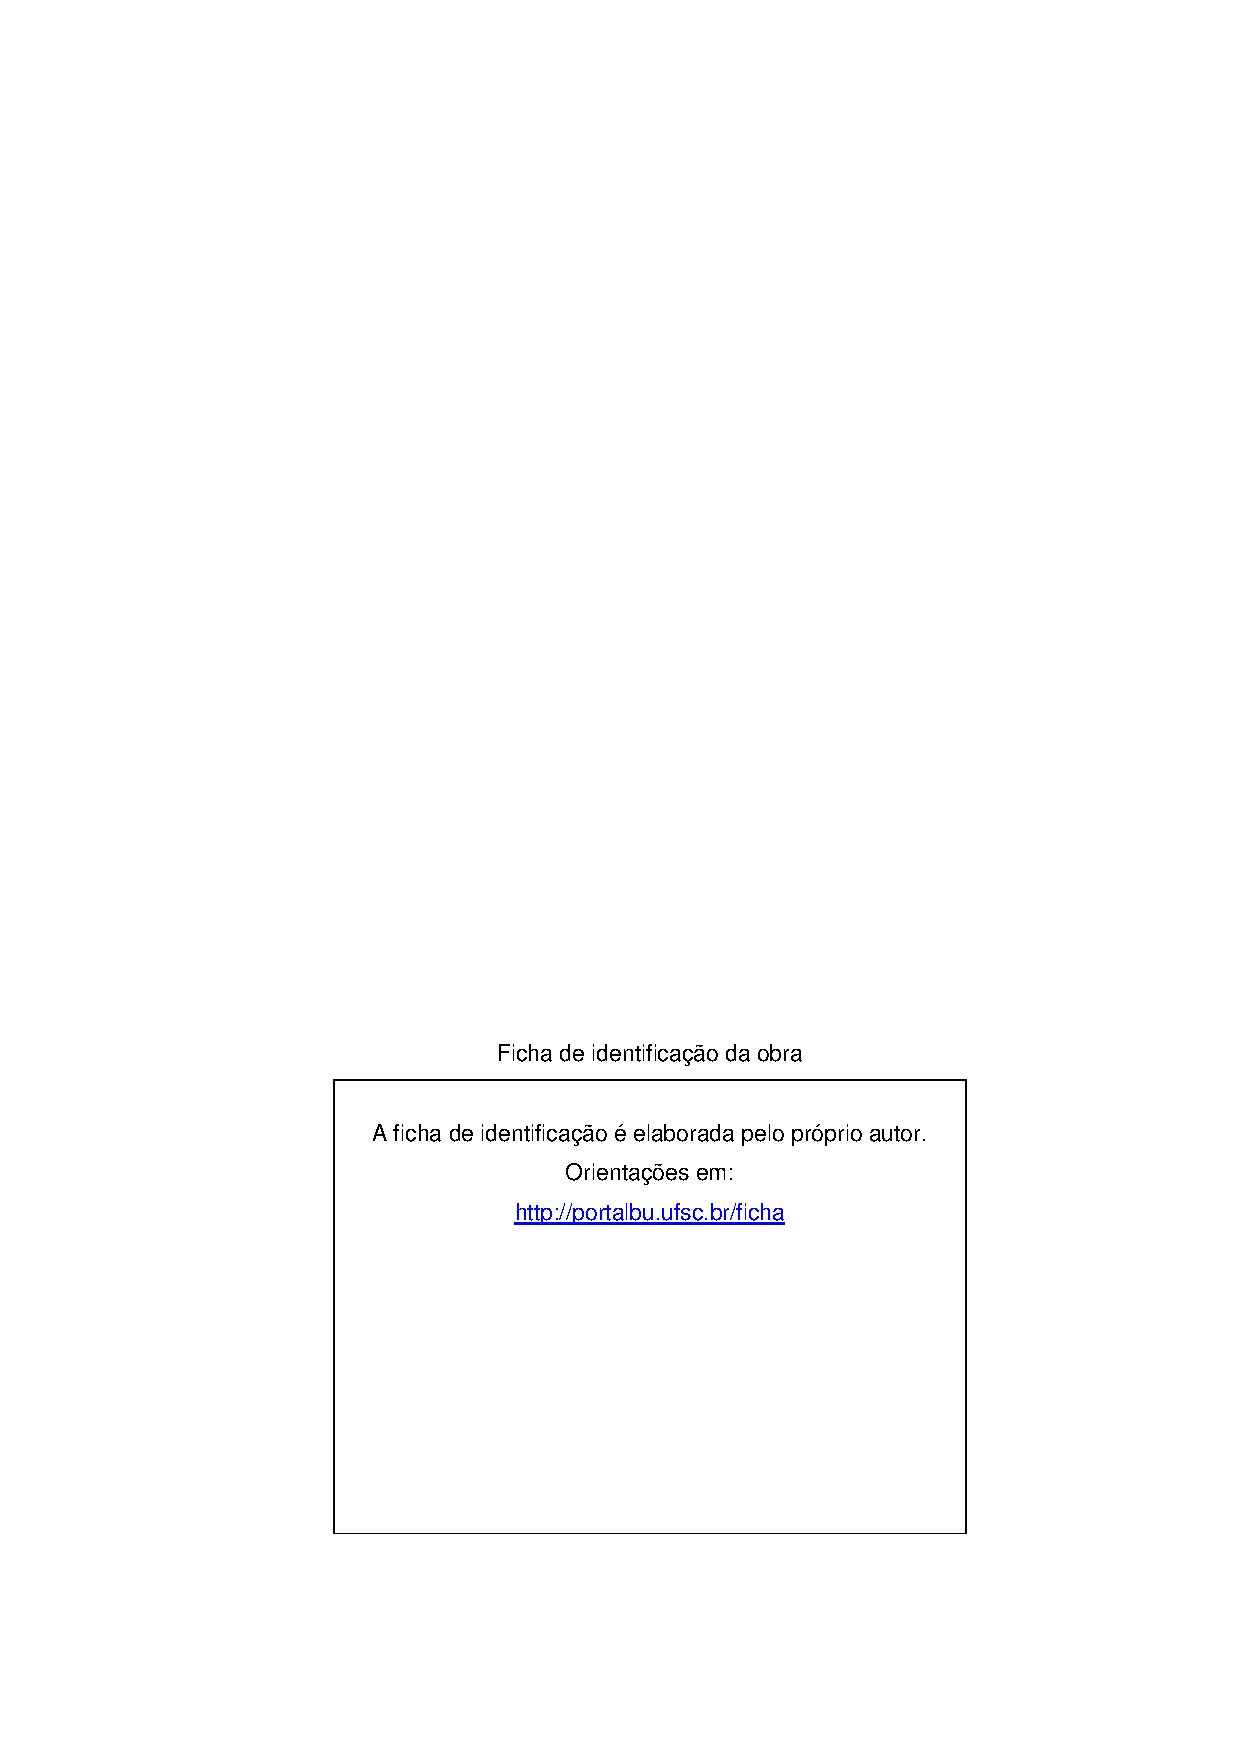
\includepdf{beforetext/Ficha_Catalografica.pdf}
\end{fichacatalografica}
% ---

% ---
% Inserir folha de aprovação
% ---
\begin{folhadeaprovacao}
	\OnehalfSpacing
	\centering
	\imprimirautor\\%
	\vspace*{10pt}		
	\textbf{\imprimirtitulo}%
	\ifnotempty{\imprimirsubtitulo}{:~\imprimirsubtitulo}\\%
	%		\vspace*{31.5pt}%3\baselineskip
	\vspace*{\baselineskip}
	%\begin{minipage}{\textwidth}
	% ~do~\imprimirprograma~do~\imprimircentro~da~\imprimirinstituicao~para~a~obtenção~do~título~de~\imprimirformacao.
	Este~\imprimirtipotrabalho~foi julgado adequado para obtenção do Título de “\imprimirformacao” e aprovado em sua forma final pelo~\imprimirprograma. \\
		\vspace*{\baselineskip}
	\imprimirlocal, \imprimirdata. \\
	\vspace*{2\baselineskip}
	\assinatura{\OnehalfSpacing\imprimircoordenador \\ \imprimircoordenadorRotulo~do Curso}
	\vspace*{2\baselineskip}
	\textbf{Banca Examinadora:} \\
	\vspace*{\baselineskip}
	\assinatura{\OnehalfSpacing\imprimirorientador \\ \imprimirorientadorRotulo}
	%\end{minipage}%
	\vspace*{\baselineskip}
	\assinatura{Prof. Pedro Luiz Borges Chaffe, Dr.\\
	Avaliador \\
	Universidade Federal de Santa Catarina}

	\vspace*{\baselineskip}
	\assinatura{Profa. Taciana Toledo de Almeida Albuquerque, Dra.\\
	Avaliadora \\
	Universidade Federal de Minas Gerais}

	\vspace*{\baselineskip}
	\assinatura{Prof. Thiago Nogueira, Dr.\\
	Avaliador \\
	Universidade de São Paulo}

	\vspace*{\baselineskip}
	\assinatura{Prof. Rizzieri Pedruzzi, Dr.\\
	Avaliador \\
	Universidade do Estado do Rio de Janeiro}

	\vspace*{\baselineskip}
	\assinatura{Prof. Alejandro Durán Carrillo de Albornoz, Dr.\\
	Avaliador \\
	Universidade de Havana, Cuba}

\end{folhadeaprovacao}
% ---

% ---
% Dedicatória
% ---
\begin{dedicatoria}
	\vspace*{\fill}
	\noindent
	\begin{adjustwidth*}{}{5.5cm}     
		Este trabalho é dedicado aos meus colegas de classe e aos meus queridos pais.
	\end{adjustwidth*}
\end{dedicatoria}
% ---

% ---
% Agradecimentos
% ---
\begin{agradecimentos}
	Inserir os agradecimentos aos colaboradores à execução do trabalho. 
	
	Xxxxxxxxxxxxxxxxxxxxxxxxxxxxxxxxxxxxxxxxxxxxxxxxxxxxxxxxxxxxxxxxxxxxxx. 
\end{agradecimentos}
% ---

% ---
% Epígrafe
% ---
\begin{epigrafe}
	\vspace*{\fill}
	\begin{flushright}
		\textit{``Texto da Epígrafe.\\
			Citação relativa ao tema do trabalho.\\
			É opcional. A epígrafe pode também aparecer\\
			na abertura de cada seção ou capítulo.\\
			Deve ser elaborada de acordo com a NBR 10520.''\\
			(Autor da epígrafe, ano)}
	\end{flushright}
\end{epigrafe}
% ---

% ---
% RESUMOS
% ---

% resumo em português
\setlength{\absparsep}{18pt} % ajusta o espaçamento dos parágrafos do resumo
\begin{resumo}
	\SingleSpacing
	O monitoramento da qualidade do ar tem experimentado uma mudança de paradigma com a incorporação de sensores de baixo custo. Estes equipamentos têm potencial para aumentar a resolução espaço-temporal dos dados de poluentes, assim como diversificar e simplificar as aplicações de monitoramento. Todavia, esses dispositivos ainda devem alcançar níveis de confiabilidade apropriados para serem utilizados de forma estendida. O volume e a diversidade de aplicações com este tipo de sensores encontra-se restrito pela baixa portabilidade de uma aplicação para outra e pela concentração de iniciativas maioritariamente em países desenvolvidos. No presente trabalho propõe-se uma solução para acelerar e facilitar o desenvolvimento e a diversificação de aplicações de monitoramento de baixo custo: a iniciativa CLEAN (Collaborative Low-cost Environmental Air quality Network). Ela consiste em uma rede colaborativa para o monitoramento de baixo custo da qualidade do ar. Os componentes da rede possuem uma arquitetura modularizada bem documentada, que possibilita o reaproveitamento de funcionalidades comuns entre aplicações. Dessa forma, os esforços de desenvolvimento podem ser direcionados à implementação dos requisitos específicos de cada aplicação particular. Dentro do marco da rede CLEAN foram desenvolvidos monitores de baixo custo. Um deles foi instalado junto a uma estação de monitoramento de referência da qualidade do ar, para validação e correção das suas leituras por um período de 5 meses. No trabalho propõe-se uma metodologia de correção das leituras do equipamento, a partir das medições coletadas pela estação de referência, utilizando modelos de regressão lineares e técnicas de aprendizado de máquinas. Durante a análise das medidas dos sensores, observou-se um alto índice de dados faltantes e alterações nos valores de linha base. Observou-se também uma correlação estatisticamente significativa entre os dados de temperatura e as leituras dos sensores de \acrshort{co}, \acrshort{o3} e \acrshort{mp10}, com coeficientes de Spearman entre 0.30 e 0.85. Os resultados obtidos nas correções, considerando as medidas de cada modelo de sensor isoladamente, foram positivos apenas nas medições de \acrshort{o3}, com um R2 máximo de aproximadamente 0.6 utilizando uma rede neural Perceptron Multicamadas e considerando a temperatura como variável de entrada no modelo. Para o restante dos sensores não foi encontrado nenhum modelo capaz de explicar a variância dos dados de concentração medidos pela estação de referência. Numa segunda iteração de processamento dos dados, aplicaram-se modelos de regressão que consideraram as leituras de todos os sensores para inferir as concentrações de um poluente. Para determinar os modelos foram testadas diferentes combinações de variáveis de entrada, técnicas de regressão e parâmetros dos modelos. As combinações que geraram os melhores resultados em termos de coeficientes de determinação foram selecionados para corrigir as leituras do equipamento de baixo custo. Dessa forma obteve-se uma melhoria nos resultados das regressões, com valores de R2 entre 0.03 e 0.5 entre todos os poluentes. A metodologia se mostrou suficientemente robusta para trabalhar com dados de baixa qualidade e acrescentar valor às leituras, sendo uma alternativa viável para equipamentos com leituras ruidosas ou falhas nos sensores. O trabalho traz como principais contribuições um marco de trabalho colaborativo para o desenvolvimento e interconexão de sensores de baixo custo, assim como uma metodologia para calibração dos sensores com dados muito ruidosos, em uma aplicação real e em ambiente não controlado.
	
	\textbf{Palavras-chave}: Monitoramento da qualidade do ar, rede colaborativa, sensores de gases de baixo custo, sistemas embarcados, \acrshort{api}, modelos de regressão, aprendizado de máquinas
\end{resumo}

% resumo em inglês
\begin{resumo}[Abstract]
	\SingleSpacing
	\begin{otherlanguage*}{english}
		Air quality monitoring has experienced a paradigm shift after incorporating  low-cost sensors. This equipments has a capability to increase the spatiotemporal resolution of pollutant data, as well as to diversify and simplify the monitoring applications. However, these devices must still reach appropriate reliability levels in order to extend its use. The volume and diversity of applications with this type of sensors is restricted by the low portability of one application to another and the concentration of initiatives mainly in developed countries. This work proposes a solution to accelerate and facilitate the development and diversification of low-cost monitoring applications: the CLEAN (Collaborative Low-cost Environmental Air Quality Network) initiative. It consists of a collaborative network for low-cost monitoring of air quality. The well documented modularized architecture of the network components allows the reusability of functionalities between applications. Thus, development efforts can be re-directed to implementing the specific requirements of each particular application. Within the framework of the CLEAN network, low-cost monitors were developed. A monitor was installed next to a certified station for monitoring air quality for a period of 5 months. This work proposes a methodology for correcting the readings of the equipment, based on measurements collected by the reference station and using linear regression models and machine learning techniques. During the analysis of sensor measurements, a high rate of missing data and changes in baseline values were observed. A statistically significant correlation was also observed between temperature data and sensor readings of \acrshort{co}, \acrshort{o3}, and \acrshort{mp10}, with Spearman coefficients between 0.30 and 0.85. The results obtained in the corrections, considering the measurements of each sensor model separately, were positive only for the measurements of \acrshort{o3}, with an R2 maximum of approximately 0.6 using a Multilayer Perceptron neural network and considering temperature as an input variable in the model. For the rest of the sensors, no model was found capable of explaining the variance of the concentration data measured by the reference station. In a second iteration of data processing, regression models were applied that considered the readings from all sensors to infer the concentrations of a pollutant. To determine the models, different combinations of input variables, regression techniques, and model parameters were tested. The combinations that generated the best results in terms of coefficient of determination were selected to correct the readings of the low-cost equipment. This way, an improvement in the regression results was achieved, with R2 values between 0.03 and 0.5 among all pollutants. The methodology proved to be robust enough to work with low-quality data and add value to readings, being a viable alternative for equipment with noisy readings or sensor failures. The main contributions of the work are a collaborative work framework for the development and interconnection of low-cost sensors, as well as a methodology for calibrating sensors with very noisy data, in a real application and an uncontrolled environment.

		\textbf{Keywords}: Air quality monitoring, collaborative network, low-cost gas sensors, embedded systems, \acrshort{api}, regression models, machine learning
	\end{otherlanguage*}
\end{resumo}

{%hidelinks
	\hypersetup{hidelinks}
	% ---
	% inserir lista de ilustrações
	% ---
	\pdfbookmark[0]{\listfigurename}{lof}
	\listoffigures*
	\cleardoublepage
	% ---
	
	% ---
	% inserir lista de tabelas
	% ---
	\pdfbookmark[0]{\listtablename}{lot}
	\listoftables*
	\cleardoublepage
	% ---
	
	% ---
	% inserir lista de abreviaturas e siglas (devem ser declarados no preambulo)
	% ---
	% \imprimirlistadesiglas
	% ---
	
	% ---
	% inserir lista de símbolos (devem ser declarados no preambulo)
	% ---
	% \imprimirlistadesimbolos
	% ---
	\printglossary[title=Lista de Siglas, toctitle=Lista de siglas]
    % \printglossary[type=\acronymtype,title=Lista de Símbolos, toctitle=Lista de símbolos]

	% ---
	% inserir o sumario
	% ---
	\pdfbookmark[0]{\contentsname}{toc}
	\tableofcontents*
	\cleardoublepage
	
}%hidelinks
% ---
% ---

% ----------------------------------------------------------
% ELEMENTOS TEXTUAIS
% ----------------------------------------------------------
\textual

% ---
% 1 - Introdução
% ---

% \phantomsection
% ----------------------------------------------------------
\chapter*{Introdução}
% ----------------------------------------------------------
\phantomsection
\addcontentsline{toc}{chapter}{INTRODUÇÃO}%
\markboth{Introdução}{Introdução}%

A poluição do ar é de grande risco para a saúde, sendo responsável pela morte de cerca de sete milhões de pessoas em todo o mundo anualmente e de variadas doenças cardiorrespiratórias \cite{who2021}. Inclusive tem sido evidenciado que o risco de sofrer doenças, ou mesmo de morte, é maior nos grupos de população mais vulneráveis e marginalizadas, como as minorias raciais/étnicas e as pessoas de baixo nível socioeconômico \cite{Jbaily2022AirGroups}. Embora quase 99\% da população mundial respire ar que excede os limites das diretrizes da OMS \cite{who2021}, a cobertura de monitoramento da qualidade do ar ainda é baixa e insuficiente \cite{Munir2019AnalysingSheffield}, especialmente em países de baixo e médio rendimento \cite{Vormittag2021AnaliseBrasil,Ferreira2022}. Um monitoramento representativo da poluição atmosférica é essencial para a gestão eficaz da qualidade do ar, já que a variabilidade espaço-temporal da concentração de poluentes é elevada, especialmente em ambientes urbanos \cite{Kumar2015,Mead2013TheNetworks}.

Os poluentes atmosféricos têm sido monitorados usando equipamentos complexos e caros em locais fixos \cite{Kang2022PerformanceReview}. Os altos custos desses instrumentos limitam sua implantação a apenas algumas estações por cidade, deixando grandes áreas geográficas descobertas \cite{Munir2019AnalysingSheffield}, restringindo a resolução espacial e a distribuição das redes de monitoramento \cite{Jiao2016CommunityStates,Kumar2015}. No Brasil, por exemplo, as redes de monitoramento instaladas cobrem apenas aproximadamente 2\% do total de municípios brasileiras, e seu desempenho a longo prazo é muitas vezes comprometido pela falta de manutenção e de pessoal qualificado \cite{Vormittag2021AnaliseBrasil}.

Buscando uma melhor compreensão do processo de poluição do ar e seus impactos, a ideia de sensoriamento em alta resolução espacial tem atraído a atenção da comunidade de qualidade do ar, e o uso de monitores de baixo custo tem ganhado popularidade \cite{Motlagh2020TowardMonitoring,Kumar2015}. Devido à sua versatilidade - dada pelas suas pequenas dimensões e seu consumo energético reduzido \cite{Lewis2018Low-costApplications} - e seus custos baixos (tanto de aquisição quanto de operação), esses dispositivos podem complementar a escassez espacial e temporal de redes certificadas de qualidade do ar e expandir o horizonte de novas aplicações de monitoramento \cite{Lewis2016EvaluatingResearch}. 

Alguns fabricantes desses dispositivos de baixo custo, como AQMesh, Vaisala, i-Blades, Libelium e Clarity fornecem, junto com suas plataformas de sensores, serviços de visualização e análise de dados, que são oferecidos como Software como Serviço (SaaS), Plataforma como Serviço (PaaS) ou Sensoriamento como Serviço. Outras iniciativas de dados abertos, lideradas por comunidades e instituições de investigação, fornecem recursos semelhantes. Alguns deles são o \textit{Habitat Map} \cite{HabitatMap2023AirCasting}, o \textit{Air Quality Egg Portal} \cite{AirQualityEgg2023AirPortal}, \textit{Sensor.Community} \cite{Sensor.Community2023LuftMap}, o \textit{PurpleAir} \cite{PurpleAir2023PurpleAirMonitoring}, \textit{Smart Citizen} \cite{SmartCitizen2023SmartCitizen}, \textit{uRADMonitor} \cite{uRADMonitor2023PM2.5URADMonitor} e \textit{IQAir}. O custo de aquisição das plataformas de sensores destas iniciativas varia entre 60,00 – 3.800,00 USD. Alguns deles disponibilizam \acrshort{api}s para registro e acesso aos dados dos monitores mas na maioria dos casos o acesso é pago e condicionado à aquisição de monitores. Em geral, essas plataformas disponibilizam os dados para visualização de forma gratuita mas o restante dos serviços tem custos adicionais. Dentre elas, apenas \textit{Sensor.Community} e \textit{Smart Citizen} fornecem guias para replicação dos dispositivos de monitoramento. 

Da revisão realizada observou-se que as iniciativas de código aberto ainda são escassas. As que existem são direcionadas a aplicações específicas com arquiteturas que não buscam facilitar o seu reaproveitamento em outras aplicações de monitoramento. Especificamente no contexto brasileiro não foram identificados empreendimentos que fabricassem monitores de baixo custo próprios. Percebeu-se assim a necessidade de uma iniciativa que não apenas provesse \textit{software} e \textit{hardware} para determinada aplicação, mas que, através da modularização e o reaproveitamento de código e \textit{hardware}, facilitasse e acelerasse o desenvolvimento de novas aplicações.

Os monitores de baixo custo da qualidade do ar ainda devem alcançar níveis de confiabilidade apropriados para serem utilizados de forma estendida \cite{Penza2020Low-costMonitoring}. A literatura reporta diversos trabalhos que buscam reduzir o erro e a incerteza das medições dos sensores de baixo custo mediante a aplicação de modelos de calibração e de compensação \cite{Maag2018ADeployments, Concas2021LOW-COSTPREPRINT}. Dentre os modelos de calibração aplicados, as regressões multivariadas paramétricas e não paramétricas têm produzido os melhores resultados \cite{Feng2019ReviewTechnology,Concas2021LOW-COSTPREPRINT}. O motivo para o sucesso das regressões multivariadas está relacionado com a sua capacidade para considerar múltiplas variáveis. Isso têm sido vantajoso para os sensores de gases, cujas respostas sofrem pelas sensibilidades cruzadas com outros compostos \cite{Lewis2018Low-costApplications}, assim como pela influência das condições ambientais, como a temperatura \cite{Popoola2016DevelopmentStability} e a umidade relativa \cite{Pang2018TheMonitoring}. Particularmente, os modelos paramétricos que utilizam regressões lineares multivariadas (\gls{mlr}, siglas em inglês) \cite{Spinelle2015FieldDioxide} costumam produzir os melhores resultados quando os sensores são expostos a concentrações elevadas de poluentes \cite{Karagulian2019ReviewMonitoring}. Nesses cenários, a dinâmica linear entre a concentração e a saída dos sensores prevalece sobre as interferências de outras variáveis \cite{Hagan2018CalibrationInstruments}. Já nos ambientes com baixos níveis de concentração, as repostas dos sensores são mais sensíveis às não-linearidades introduzidas pelas variações da temperatura e da umidade \cite{Hagan2018CalibrationInstruments}. Nessas condições, os modelos não paramétricos superam o desempenho da \gls{mlr} \cite{Karagulian2019ReviewMonitoring}. Embora as regressões multivariadas, especialmente as não paramétricas, tenham alavancado o uso de monitores de baixo custo, ainda é necessário buscar modelos e metodologias de calibração e correção dos dados que se adaptem às condições e características de operação de cada aplicação de sensoriamento \cite{Concas2021LOW-COSTPREPRINT}.

Diante do exposto e pelas lacunas observadas, o presente trabalho descreve o desenvolvimento de uma iniciativa para facilitar a colaboração no desenvolvimento de redes de monitoramento de baixo custo e a sua aplicação num cenário real de monitoramento. Sendo assim, define-se como \textbf{objetivo geral} da tese desenvolver uma rede colaborativa de medidores de baixo custo para monitoramento da qualidade do ar. Para isso foram definidos como objetivos específicos:

\begin{enumerate}
    \item Desenvolver dispositivos de medição para serem adicionados à rede de monitoramento
    \item Disponibilizar uma \acrshort{api} para registro dos dados de monitoramento e acesso a eles em tempo real, assim como bibliotecas de \textit{firmware} para o desenvolvimento dos dispositivos e sua comunicação com a \acrshort{api}
    \item Identificar erros e interferências nas leituras de um equipamento de baixo custo e comparar as leituras com os dados de uma estação de monitoramento de referência
    \item Desenvolver uma metodologia de correção de leituras ruidosas ou em situação de falha de sensores
\end{enumerate}

A iniciativa desenvolvida, sob o nome de CLEAN (Collaborative Low-cost Environmental Air-quality Network), inclui uma \textit{api} aberta para registro e acesso de dados de monitores de baixo custo, bibliotecas de \textit{software} bem documentadas para o desenvolvimento do \textit{firmware} dos monitores e soluções de \textit{hardware} (com documentação e tutoriais) para determinadas aplicações. A \acrshort{api} permite que diversos dispositivos de monitoramento de baixo custo enviem seus dados geo-localizados para um servidor remoto para visualização e armazenamento em tempo real. Além disso, a API possibilita a integração com outras aplicações Web para visualização e análise de dados. Esses dados permanecem abertamente disponíveis para posterior processamento e análise. CLEAN também facilita a incorporação de novos periféricos e sensores de hardware, reutilizando o código das bibliotecas e garantindo a interação com a \acrshort{api} independentemente do \textit{hardware} desenvolvido para cobrir determinada aplicação de monitoramento. Dada a grande versatilidade dos sensores de baixo custo, muitas aplicações poderiam ser monitoradas a partir de diversos cenários contribuindo para uma maior disponibilidade de volumes de dados.

Os dispositivos de \textit{hardware} desenvolvidos para a rede foram dois protótipos de monitores de baixo custo e três equipamentos com placas de circuito impresso. Estes últimos são denominados de monitores CLEAN Arduino Mega para fins de versionamento e identificação. Os cinco dispositivos utilizam sensores de gases eletroquímicos (\gls{ec}) sensíveis aos poluentes \acrshort{co}, \acrshort{no2}, \acrshort{so2}, \acrshort{o3} e \acrshort{mp}. Foram escolhidos esses gases por serem gases de referência para indicar a qualidade do ar segundo definido na Resolução no 491/2018 do \gls{conama}. Os resultados obtidos com os dois protótipos foram apresentados no congresso internacional CMAS 2020 \cite{Campo2020DEPLOYMENTRESULTS} e encontram-se fora do escopo da presente tese. Um dos monitores CLEAN Arduino Mega foi instalado no município de Tubarão, no estado de Santa Catarina, junto a uma estação de referência, para análise e correção dos seus dados. São aplicadas metodologias de pré-processamento e correção dos dados utilizando modelos multivariados baseados em \gls{mlr}, \gls{knn}, \gls{rf}, \gls{ann}. Os resultados são comparados em termos de R2, erro, e correlação com as medições de referência. 

No Capítulo \ref{cap:air-quality-monitoring} apresenta-se uma revisão bibliográfica sobre o estado da arte no monitoramento da qualidade do ar, tanto o realizado para fins regulatórios como o de baixo custo, com especial foco no estado das redes de monitoramento no Brasil. No Capítulo \ref{cap:clean-initiative} é apresentada a iniciativa CLEAN e seus componentes, i.e.: a \acrshort{api}; as bibliotecas de \textit{firmware} e os dispositivos de \textit{hardware} desenvolvidos; e a aplicação \textit{Web} \textit{Renovar}. A iniciativa CLEAN foi também apresentada em artigo científico na revista Environmental Modelling \& Software \cite{Campo2021}. O código principal dos dispositivos de monitoramento e as bibliotecas de \textit{firmware} possuem registro de programa de computador no Instituto Nacional de Propriedade Industrial com número de registro BR512022001116-6. No Capítulo \ref{cap:field-monit-results} são apresentadas as medições realizadas pelo equipamento instalado em campo, as metodologia aplicadas para pré-processar os dados e corrigi-los utilizando modelos de regressão multivariados. Por último no Capítulo \ref{cap:calib-methodology} apresenta-se a metodologia aplicada para aprimorar os resultados obtidos no Capítulo \ref{cap:field-monit-results}.
% ---

% ---
% 2 - Capítulo 1
% ---
% ----------------------------------------------------------
\chapter{Monitoramento da qualidade do ar}\label{cap:air-quality-monitoring}
% ----------------------------------------------------------

O monitoramento da poluição atmosférica se faz indispensável para o estudo e a gestão efetiva da qualidade do ar. O monitoramento considerado de referência é realizado por instituições governamentais através de redes de monitoramento automáticas \cite{Franca2019GUIAAR}. Essas redes são compostas por estações de monitoramento, certificadas por órgãos competentes, as quais registram ininterruptamente, e em tempo real, as concentrações dos poluentes na atmosfera \cite*{CETESB2020RedesAr}. As estações podem ser fixas ou móveis e a qualidade das suas leituras é garantida mediante procedimentos padrões de calibração dos instrumentos, de coleta de dados e de pós-processamento. As informações coletadas são processadas com base nos padrões legais estabelecidos e podem ser disponibilizados na forma de boletins diários ou relatórios anuais, como um resumo das condições da poluição atmosférica dentro de determinada área \cite{CETESB2020RedesAr}. No Brasil, para facilitar o entendimento e a divulgação da informação da qualidade do ar de curto prazo, é utilizado o Índice da Qualidade do Ar \gls{iqar}. Este índice é um valor adimensional que outorga uma nota de Boa até Péssima à qualidade do ar, relacionando a informação quantitativa de concentração de determinados poluentes com seus efeitos na saúde humana \cite{Franca2019GUIAAR}. Os poluentes que são regulados pela legislação brasileira, na Resolução no. 491/2018, e que portanto são medidos pelas redes de monitoramento de referência são: o material particulado (\acrshort{mp}), as partículas totais em suspensão, o dióxido de enxofre (\acrshort{so2}), o dióxido de nitrogênio (\acrshort{no2}), o ozônio ao nível de solo (\acrshort{o3}), o monóxido de carbono (\acrshort{co}) e a fumaça.

As redes de monitoramento de referência caracterizam-se por uma elevada precisão e confiabilidade. Contudo, fatores como preço, consumo energético, complexidade de operação e dimensões acabam dificultando seu uso de forma mais extensa. A literatura reporta preços dessas tecnologias em torno de \$ 15.000 – \$ 100.000 \cite{Concas2021LOW-COSTPREPRINT} e consumo de potência aproximadamente entre 0.2 e 1 kW \cite{Piedrahita2014TheMonitoring}, sem contar os custos advindos dos procedimentos de manutenção \cite{Kumar2015}. Sendo assim, a onerosidade da solução como um todo limita o número de estações financeiramente viáveis e reduz a resolução e distribuição espacial das medições, inclusive em países e regiões com elevados índices de desenvolvimento econômico como os Estados Unidos e a Europa \cite*{Kumar2015,Jiao2016CommunityStates}.

No Brasil o monitoramento de referência é ainda bastante limitado. Algumas iniciativas governamentais e de órgãos de pesquisa, a nível nacional e estadual, têm sido implementadas para facilitar o acesso a dados sobre a qualidade do ar como, por exemplo: \cite{CETESB2020RedesAr}, \cite{IEMA2020QualidadeAr} e \cite{IEMA/ES2020IEMAAr}. No entanto, ainda assim, as redes de monitoramento que têm sido instaladas cobrem escassos pontos das cidades brasileiras e seu desempenho a longo prazo muitas vezes se vê comprometido por falta de manutenção e de pessoal qualificado \cite{Oyama2017AIRBRAZIL}. Segundo um estudo de 2019 realizado pelo Instituto Saúde e Sustentabilidade, das 27 unidades federativas apenas 7 monitoram a qualidade do ar e atendem o regulamento vigente. O restante das unidades não realizam o monitoramento ou o realizam de forma ineficiente \cite{InstitutoSaudeeSustentabilidade2019AnaliseBrasil}. O estudo também aponta que das 319 estações ativas no país, a região sudeste concentra o 93\% delas. O estado de Santa Catarina, em particular, não realiza monitoramento da qualidade do ar.

A pesar da sua elevada confiabilidade, devido à sua limitada distribuição espacial, as redes de monitoramento de referência da qualidade do ar proveem apenas informações globais relativas a níveis de concentrações de fundo, o que dificulta a compilação de informação confiável e representativa de áreas específicas \cite{Kumar2015}. Esse fato constitui uma limitante para o estudo dos processos associados à poluição atmosférica. Dada a alta variabilidade espaço-temporal da concentração dos poluentes, especialmente em ambientes urbanos \cite{Mead2013TheNetworks}, a resolução espacial das redes de monitoramento é tão relevante quanto a confiabilidade das suas estações \cite{Jiao2016CommunityStates}.

Diante disso, se faz necessário a busca de novas soluções que possibilitem incrementar o número de monitores viáveis nas redes de monitoramento sem afetar a qualidade das medições. Todavia, especial cuidado deve ser tomado para não comprometer a qualidade dos dados obtidos, já que, como apontado por Emily Snyder e colaboradores, ter dados pouco confiáveis é mais prejudicial do que não ter dados, pois podem conduzir a decisões desacertadas \cite{Snyder2013}.

Com o intuito de regulamentar o uso de monitores de baixo custo segundo a confiabilidade das suas leituras, a Diretiva Europeia para a Qualidade do Ar definiu o Objetivo da Qualidade dos Dados (\gls{dqo}) como requisito necessário para o uso destes instrumentos para fins de indicação da concentração de poluentes atmosféricos \cite{EU2008DirectiveEurope}. O \gls{dqo} representa o nível de incerteza aceitável nas medições destes instrumentos sendo de 50\% para \acrshort{mp}, 30\% para \acrshort{o3} e 25\% para \acrshort{co}, \acrshort{nox} e \acrshort{so2}. A Agência de Proteção Ambiental Norte-americana (\gls{epa}), por outro lado, sugere a avaliação dos instrumentos de monitoramento considerando cinco áreas de aplicação (Tabela \ref{tab:monitoring-areas-EPA}). Cada área tem valores de precisão, viés e completude dos dados que devem ser cumpridos para que um monitor de baixo custo possa ser utilizado em aplicações dentro dessa área \cite{Williams2014AirGuidebook}. Numa direção um pouco diferente dos dois órgãos anteriores, em um estudo mais recente conduzido por Lidia Morawska, foi proposto que, dado o amplo leque de aplicações de monitoramento, os requisitos de desempenho dos monitores de baixo custo fossem definidos de acordo com cada aplicação prescindindo assim de métricas padrões \cite{Morawska2018ApplicationsGone}. Esta última abordagem, contudo, exige um conhecimento profundo da aplicação e dos requerimentos de desempenho associados \cite{Morawska2018ApplicationsGone}.

\begin{table}[t]
    \caption{Requerimentos de desempenho dos instrumentos de monitoramento da qualidade do ar segundo área de aplicação}
    \begin{tabular}{ 
    | m{0.35\textwidth} m{0.3\textwidth} m{0.10\textwidth} m{0.15\textwidth} | }
        \hline
        Área de aplicação & Poluentes & Erro & Completude dos dados \\ [0.5ex] 
        \hline
        Educação e Informação & Todos & < 50\% & $\geq$ 50\% \\ [0.5ex]
        \hline
        Identificação e Caracterização de \textit{Hotspots}\footnotemark & Todos & < 30\% & $\geq$ 75\% \\ [0.5ex]
        \hline
        Monitoramento Complementar & Todos os regulados pelo \gls{conama} e os \acrshort{voc} & < 20\% & $\geq$ 80\% \\ [0.5ex]
        \hline
        Exposição pessoal & Todos & < 30\% & $\geq$ 80\% \\ [0.5ex]
        \hline
        Monitoramento de referência & \acrshort{o3} \newline \acrshort{co}, \acrshort{so2} \newline \acrshort{no2} \newline \acrshort{mp} & < 7\% \newline < 10\% \newline < 15\% \newline < 10\% & $\geq$ 75\% \\ [0.5ex]
        \hline
    \end{tabular}
    \label{tab:monitoring-areas-EPA}
    \fonte{\cite{Williams2014AirGuidebook}}
\end{table}
\footnotetext{Pontos de elevada concentração de determinado poluente}

% ----------------------------------------------------------
\section{Importância}
% ----------------------------------------------------------

Importância (Efeitos da poluição atmosférica e necessidade de monitoramento para controle)

% ----------------------------------------------------------
\section{Monitoramento de referência}
% ----------------------------------------------------------

(custos, equipamentos, técnicas)

% ----------------------------------------------------------
\section{Monitoramento de baixo custo da qualidade do ar}\label{section:low-cost-air-quality-monit}
% ----------------------------------------------------------

% (estado atual, vantagens, desvantagens e desafios, Brasil)

Segundo Emily Snyder e colaboradores  o monitoramento da qualidade do ar tem experimentado uma mudança de paradigma na forma como os dados são coletados \cite{Snyder2013}. Os avanços recentes em instrumentação eletrônica unido a necessidade de soluções alternativas que complementem as técnicas de monitoramento tradicionais, têm contribuído para um crescente interesse no desenvolvimento de sensores de qualidade do ar de baixo custo \cite{Kumar2015,Lewis2018Low-costApplications}. Esses novos sensores possuem características essenciais como tamanho e peso reduzidos, baixo consumo de potência, baixo custo e facilidade de uso, que os colocam em vantagem com relação aos instrumentos de referência, e que têm criado as condições para aprimorar uma série de aplicações de monitoramento e gerar novas \cite{Snyder2013,Lewis2018Low-costApplications}.

Este tipo de tecnologia possibilitaria a agências públicas, entidades reguladoras e de pesquisa utilizar um maior volume de sistemas de monitoramento, e assim diversificar e complementar as aplicações de monitoramento para fins de pesquisa e regulamentação e validar modelos atmosféricos \cite{Lewis2018Low-costApplications}. Estes sistemas podem prover informação temporal qualitativa relevante sobre o nível de poluição atmosférica em uma determinada localidade por períodos de dias a meses \cite{Castell2018LocalizedNodes}, como por exemplo, os momentos do dia em que a poluição é maior ou menor \cite{Zimmerman2018AMonitoring}, ou observar a sua variação ao longo do tempo \cite{Castell2017CanEstimates}. Igualmente, os sistemas de baixo custo têm sido utilizados para detectar de áreas com níveis de concentração elevados nas cidades \cite{Mead2013TheNetworks} e elaborar mapas de poluição \cite{Huang2019EstimatingMeasurements}.

Para Emily Snyder e colaboradores o uso deste tipo de sensores pode levar a uma melhor proteção da saúde pública e do meio ambiente \cite{Snyder2013}. Sensores de baixo custo podem ser usados para prover informação representativa de exposição pessoal a poluentes, com elevada resolução temporal \cite{Mead2013TheNetworks,Jerrett2017ValidatingScience}. Igualmente, esta nova forma de medição, por ser de baixo custo e de fácil operação, pode ser instalada em comunidades \cite{Mahajan2020APollution}, escolas e áreas residenciais \cite{Castell2018LocalizedNodes}, provendo informação à população sobre a qualidade do ar que respiram, e colocando os processos de monitoramento e medição nas mãos de comunidades e indivíduos \cite{Lewis2018Low-costApplications}.

Segundo seu princípio de funcionamento, os sensores de baixo custo utilizados para a medição de poluentes na atmosfera podem ser classificados em: sensores de material particulado e sensores de gases \cite{Maag2018ADeployments}. Os sensores de material particulado funcionam baseados em princípios  de detecção óticos que medem o espalhamento ou a adsorção da luz pelas partículas \cite{Rai2017End-userMonitoring}. Já os sensores de gases podem ser subdivididos em duas classes: os óticos e os que dependem da interação entre o material transdutor e o composto gasoso \cite{Snyder2013}.
	
O princípio ótico de medição consiste em expor o composto gasoso a um feixe de luz, com determinado comprimento de onda, e medir o efeito dessa interação com um detector fotossensível \cite{Rai2017End-userMonitoring}. Dentro desse grupo, os sensores mais comuns são os infravermelhos não-dispersivos (\gls{ndir}, por suas siglas em inglês), usados para medir \acrshort{co2} e \acrshort{ch4}, e os detectores de foto-ionização (\gls{pid}, por suas siglas em inglês) que utilizam luz ultravioleta e são usados para medir compostos orgânicos voláteis \cite{Snyder2013}.

Dentre os sensores de gases que operam a partir da interação entre o material transdutor e o composto gasoso, os mais populares são: os semicondutores de óxido metálico (\gls{mos}, por suas siglas em inglês) e os de princípio eletroquímico (\gls{ec}, por suas siglas em inglês). Esses são os sensores mais comumente utilizados para medir gases tóxicos como \acrshort{co}, \acrshort{nox}, \acrshort{o3} e \acrshort{so2} \cite{Lewis2018Low-costApplications}.

Os sensores \gls{ec}, em comparação com os \gls{mos}, costumam ter um menor consumo de potência, maior seletividade, menores limites de detecção e uma relação linear com a concentração. Os sensores \gls{mos}, por sua parte, têm custos menores e seu condicionamento eletrônico costuma ser mais simples \cite{Rai2017End-userMonitoring}. Neste trabalho serão abordados apenas os sensores eletroquímicos por serem os mais utilizados para o monitoramento de baixo custo da qualidade do ar e pela relação linear entre suas respostas e a concentração de gás.

É importante ressaltar que o atual estado da arte dos sensores de baixo custo impossibilita que eles substituam os métodos de medição de referência. Contudo, resultados promissores têm sido encontrados em várias áreas, principalmente naquelas em que as técnicas convencionais não poderiam ser implementadas devido a limitações como a pouca portabilidade, o elevado consumo energético e o custo. 

% ----------------------------------------------------------
\subsection{Limitações do monitoramento de baixo custo da qualidade do ar}\label{subsection:low-cost-monit-limits}
% ----------------------------------------------------------

Os sensores de gases de baixo custo, como qualquer sistema de medição, possuem fontes de erro internas que são inerentes ao seu próprio funcionamento \cite{Maag2018ADeployments}. Estes erros são geralmente conhecidos e fáceis de determinar. Além desses, existem fontes de interferência externas, relacionadas às suas condições de operação, que são mais difíceis de detectar e controlar. Inclusive, sensores de um mesmo fabricante e de um mesmo lote de fabricação, podem apresentar comportamentos diferentes perante a influência de fontes externas \cite{Alphasense2013AlphasenseHUMIDITY,Castell2017CanEstimates}.

Os fabricantes normalmente definem um intervalo de medição onde os sensores apresentam melhor desempenho. O limite inferior desse intervalo é conhecido como limite de detecção, e todos os valores inferiores a ele são considerados como ruído \cite{Maag2018ADeployments}. Esse parâmetro é determinado em condições de laboratório, por isso em condições de operação não controladas, o seu valor pode sofrer alterações levando a erros nas medições. Por exemplo, em ambientes com muitas fontes de ruído electromagnético, ou um circuito de alimentação de energia pouco robusto a flutuações na tensão elétrica, podem aumentar a amplitude do ruído elétrico e, com ele, o limite de detecção dos sensores, afetando a sua resolução.

Outro tipo de erro sistemático que se manifesta internamente são os erros de offset e de sensibilidade. Como estes erros são não aleatórios são relativamente fáceis de remover mediante calibrações de laboratório \cite{Spinelle2013ProtocolPollution}. As derivas são outra fonte interna de erros produto de alterações na sensibilidade dos sensores devido principalmente ao seu envelhecimento, que dificultam seu uso para monitoramento a longo prazo \cite{Feng2019ReviewTechnology}. As derivas podem ser eliminadas com re-calibrações periódicas. A frequência das re-calibrações depende do sensor e da concentração de poluentes a que é exposto, podendo chegar a ser quinzenal \cite{Concas2021LOW-COSTPREPRINT}.

Fatores externos ao funcionamento dos sensores também produzem interferências nas medições. A influência desses fatores, principalmente das condições ambientais, são identificados por grande parte dos autores como um dos principais desafios no tratamento das respostas dos sensores \cite*{Mead2013TheNetworks,Popoola2016DevelopmentStability,Rai2017End-userMonitoring,Baron2017AmperometricReview}. Esses problemas são característicos de medições feitas em ambientes externos, em condições e ambientes reais, não controladas, ao contrário das medições tomadas em condições de laboratório sob as quais o desempenho dos sensores costuma ser muito melhor \cite{Castell2017CanEstimates}.

Variações na temperatura e na umidade do ambiente afetam a sensibilidade e o valor de linha base dos sensores \cite{Popoola2016DevelopmentStability,Pang2018TheMonitoring}. Particularmente, tem sido observado que em ambientes externos, onde os níveis de concentração costumam encontrar-se na ordem dos \gls{ppb}, as variações na temperatura e na umidade relativa alteram o valor de linha base em maior medida que a sensibilidade \cite{Popoola2016DevelopmentStability}.

Os fabricantes de sensores muitas vezes disponibilizam informações sobre a relação entre as respostas dos sensores e as variáveis ambientais, junto a modelos lineares de compensação \cite{Alphasense2013AlphasenseHUMIDITY,SPECSensors2016ApplicationPerformance}. No entanto, essas informações são obtidas a partir de testes de laboratório que simulam condições reais \cite{Spinelle2013ProtocolPollution}, sendo válidas apenas em níveis de concentração na ordem dos \gls{ppm} e em condições similares às dos testes \cite{Lewis2018Low-costApplications}. Dessa forma, as soluções para compensar os efeitos da temperatura e a umidade relativa providas pelos fabricantes resultam insuficientes para aplicações em campo \cite{Pang2018TheMonitoring}. Essas informações são especialmente limitadas para aplicações de monitoramento móvel, onde os sensores são expostos a transientes de concentração bruscos e condições ambientais variadas \cite{Delaine2019InReview}.
	
Uma solução que o fabricante Alphasense tem aplicado nos seus sensores é a incorporação de um quarto eletrodo, chamado eletrodo auxiliar, cujo sinal de saída é utilizado para compensar os efeitos de variáveis ambientais no valor de linha base do sensor \cite{Alphasense2019AlphasenseSensors}. Este eletrodo tem uma composição similar ao eletrodo de trabalho e provê um sinal de corrente de linha base que acompanha as variações do eletrodo de trabalho decorrentes das mudanças na temperatura, a umidade relativa e a pressão, podendo ser subtraída para obter a resposta do sensor ao gás \cite{Baron2017AmperometricReview}. Idealmente deveria funcionar assim, contudo, na prática tem sido demonstrado que o eletrodo auxiliar não é capaz de acompanhar as variações do eletrodo de trabalho em todo o intervalo de temperaturas de operação, e que portanto, uma simples subtração é insuficiente para gerar uma resposta confiável \cite{Wei2018ImpactMonitoring}. Cross e colaboradores também comprovaram que as correções recomendadas pelo fabricante Alphasense utilizando o eletrodo auxiliar não produzem os níveis de acurácia requeridos nas medições em ambientes externos \cite{Cross2017UseMeasurements}.
	
Tem sido reportado que variações bruscas na umidade relativa e na pressão ambiente produzem picos nas respostas dos sensores que invalidam as leituras por intervalos de tempo de até 40 minutos \cite{Alphasense2013AlphasenseHUMIDITY,Lewis2018Low-costApplications}. Igualmente ambientes com valores de umidade muito extremos ou muito poluídos podem saturar os sensores ocasionando falhas e reduzindo sua sensibilidade \cite{Alphasense2013AlphasenseHUMIDITY}.

Outros fatores que influenciam no desempenho dos sensores são as variações nos níveis de concentração do local de instalação. Os sensores eletroquímicos, por exemplo costumam ter melhor desempenho em locais onde os níveis de poluição são elevados \cite{Castell2017CanEstimates}, já que nestas condições a dinâmica senso-gás predomina sobre o efeito das variáveis interferentes \cite{Hagan2018CalibrationInstruments}. Por exemplo, Hagan e colaboradores comprovaram que o efeito da umidade relativa poderia ser ignorado ao calibrar um sensor \gls{ec} sensível a \acrshort{so2} em todo o intervalo de medição do sensor, contudo, para medições abaixo de 25 ppb, o efeito da umidade relativa mostrou-se significativa \cite{Hagan2018CalibrationInstruments}. Nuria Castell e colaboradores obtiveram coeficientes de correlação maiores com sensores instalados em locais com trânsito intenso do que nos locais com trânsito leve \cite{Castell2017CanEstimates}. Eles também constataram que o coeficiente de correlação dos sensores testados em locais com trânsito intenso caiu de forma considerável durante o período de férias, quando o trânsito pelo local foi reduzido \cite{Castell2017CanEstimates}. Por esse motivo, outro dos desafios dos monitores de baixo custo é que os instrumentos mantenham um bom desempenho independentemente dos níves de concentração encontrados no local \cite{Concas2019ACalibration}.

Outro problema comum dos sensores de baixo custo é a sensibilidade cruzada, que é a sensibilidade que os sensores têm a outros gases além do gás de interesse \cite{Maag2018ADeployments}. Por exemplo, é bem conhecido que os sensores de \acrshort{o3} são também sensíveis ao \acrshort{no2} \cite{Pang2017ElectrochemicalMonitoring,Alphasense2019AlphasenseSensors}. Outros estudos têm encontrado também sensibilidade a \acrshort{no2} em sensores de \acrshort{no} e \acrshort{so2} \cite{Lewis2016EvaluatingResearch}, assim como a \acrshort{o3} e \acrshort{co2} em sensores de \acrshort{no2} \cite{Lewis2018Low-costApplications}. Este efeito é especialmente desvantajoso em ambientes externos onde o ar é formado por uma mistura complexa de compostos gasosos. Por isso, se faz necessário assegurar que a leitura de um sensor corresponda ao gás para o qual foi projetado sem a interferência de outros compostos.

Uma forma de abordar o problema da sensibilidade cruzada é otimizando o material do eletrodo de trabalho durante a fabricação do sensor, para facilitar ou catalisar apenas as reações do gás de interesse \cite{R.Stetter2008AmperometricReview}. Igualmente, a seletividade pode ser melhorada no circuito de condicionamento, fixando o potencial de trabalho em um valor que favoreça as reações para o gás objeto de estudo \cite{R.Stetter2008AmperometricReview,Alphasense2013AlphasenseWork}. Em ambientes externos essas abordagens costumam ser insuficientes, sendo necessário utilizar arranjos de sensores nas medições e aplicar técnicas de calibração multivariadas que considerem a resposta global do arranjo \cite{Maag2018ADeployments}.

Dada a multiplicidade e complexidade dos fatores que influenciam as medições dos sensores de baixo custo, se faz necessário o estudo cuidadoso e a aplicação de técnicas de calibração que garantam níveis de precisão e confiabilidade aceitáveis para cada aplicação de monitoramento. Isso é de importância especialmente nas aplicações de monitoramento móvel, em que os sensores são expostos a transientes bruscos nas condições de operação.
% ---

% ---
% 2 - Capítulo 2
% ---
% ----------------------------------------------------------
\chapter{CLEAN - Collaborative Low-cost Environmental and Air-quality Network}\label{cap:clean-initiative}
% ----------------------------------------------------------

A iniciativa CLEAN consiste numa plataforma colaborativa de código aberto para promover e facilitar o desenvolvimento de monitores de qualidade do ar de baixo custo e o acesso remoto a informações sobre a qualidade do ar em tempo real. Possui três componentes principais, conforme enumerado a seguir e ilustrado de forma gráfica na Figura \ref{fig:clean-structure}.

\begin{enumerate}
    \item API Renovar para acesso aos dados de dispositivos de monitoramento
    \item Bibliotecas de \textit{firmware} baseadas no framework Arduino para programação dos dispositivos de monitoramento e comunicação com a \textit{api}
    \item Aplicação \textit{web} \href{http://renovar.lcqar.ufsc.br/}{Renovar} para visualização e análise dos dados na forma de mapas, séries históricas e gráficos de \textit{box-plot}
\end{enumerate}

\begin{figure}[h]
    \centering
    \caption{Componentes da iniciativa CLEAN}
    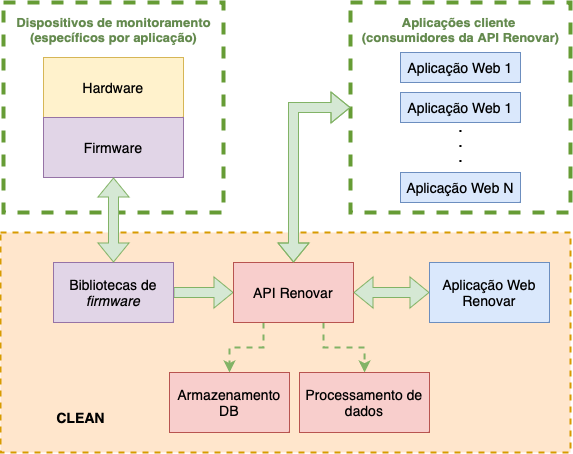
\includegraphics[width=0.80\linewidth]{chapters//2-CLEAN//Figuras/Estrutura CLEAN.png}
    \label{fig:clean-structure}
    \fonte{Desenvolvido pelo autor (2023)}
\end{figure}

Além disso, a iniciativa disponibiliza a documentação do \textit{hardware} e do \textit{firmware} dos monitores desenvolvidos dentro desse contexto para facilitar a sua replicação e a colaboração entre os diferentes agentes. Todos os guias e documentação relativos ao desenvolvimento do hardware e firmware dos dispositivos até agora concebidos, as bibliotecas implementadas e as ferramentas de desenvolvimento estão abertas e disponíveis gratuitamente na página inicial de CLEAN \cite{Campo2021}.

A \acrshort{api} Renovar disponibiliza os recursos necessários para a comunicação remota com dispositivos de monitoramento, o registro das leituras dos dispositivos e o acesso aos dados para visualização, processamento e análise. Dentro da iniciativa CLEAN pretende-se que a \acrshort{api} seja uma forma de centralizar o registro (através de dispositivos de monitoramento) e o acesso (através de aplicações cliente) a dados da qualidade do ar de monitores de baixo custo desenvolvidos por parceiros, eximindo eles da necessidade de desenvolver soluções próprias desde zero. Assim, CLEAN pretende acelerar e facilitar a expansão de aplicações de monitoramento de baixo custo e de análise de dados. 

As bibliotecas de \textit{firmware} providenciam uma interface entre o \textit{hardware} e \textit{firmware} específico para cada aplicação de monitoramento e a \acrshort{api}, facilitando também o processo de desenvolvimento, e permitindo aos parceiros focarem na aplicação em si, sem investir muito esforço na integração com a \acrshort{api}. As bibliotecas de \textit{firmware} também providenciam abstrações para os componentes de \textit{hardware}, como sensores, controladores e periféricos, contribuindo ao reaproveitamento de código. A medida que os parceiros forem incorporando novos componentes nas suas aplicações, novas abstrações podem ser adicionadas às bibliotecas, expandindo o leque de interfaces a componentes de \textit{hardware}.

A aplicação \textit{web} Renovar desenvolvida dentro do contexto de CLEAN é uma aplicação \textit{front-end} consumidora da \acrshort{api}. Ela é uma alternativa para iniciar qualquer aplicação de monitoramento de baixo custo já que disponibiliza a visualização de mapas dos dispositivos, séries temporais dos dados dos sensores e gráficos de \textit{box-plots} dos dados. Pode funcionar também como modelo para outras aplicações consumidoras que venham a ser desenvolvidas.

% ----------------------------------------------------------
\section{Bibliotecas de firmware}
% ----------------------------------------------------------

O \textit{firmware} dos dispositivos foi desenvolvido no \textit{Framework Arduino}, que é uma abstração de códigos-fonte e bibliotecas comuns a diversas plataformas de \textit{\textit{hardware}}. Esta estrutura torna possível escrever programas para controlar uma ampla gama de placas microcontroladoras de Arduino e de outros fabricantes. O \textit{framework} fornece bibliotecas de código escritas em C/C++ para programação de microcontroladores e interação com dispositivos periféricos.

Para programar todas as funcionalidades do \textit{firmware} CLEAN, o código foi estruturado em um conjunto de classes em C++. Esta estrutura foi concebida visando sua reutilização em outras plataformas de microcontroladores e outros componentes de \textit{hardware} suportados no Framework Arduino (como ESP8266 da Espressif) e também para facilitar a revisão e manutenção do código. As classes desenvolvidas para o projeto estão distribuídas em quatro módulos principais, conforme mostrado na Figura \ref{fig:fw-libraries-structure}: o módulo \textit{Hardware Interfaces}, o módulo \textit{System Drivers}, o módulo \textit{}{Sensors} e o módulo \textit{Data}.

O módulo \textit{Hardware Interfaces} agrupa todas as classes e estruturas utilizadas para se comunicar com o \textit{hardware} periférico, como sensores, módulos de temporização, módulos de geolocalização e módulos de armazenamento. Os \textit{Drivers} implementam funcionalidades que podem ser utilizadas pelo programa principal independentemente do \textit{hardware} utilizado em cada dispositivo. O pacote \textit{Sensors} está no mesmo nível dos \textit{Drivers} e pode ser interpretado como um conjunto de \textit{drivers} especiais para os sensores, mas com a particularidade de ser específico para cada fabricante. Por fim, o pacote Dados engloba todas as funcionalidades relacionadas à preparação de dados de sensores para armazenamento e transmissão. Este pacote abstrai as informações de concentração adquiridas pelos sensores de gás a partir de detalhes específicos sobre o funcionamento e operação de seu \textit{hardware}.

\begin{figure}[h]
    \centering
    \caption{Conjunto de bibliotecas utilizadas para \textit{firmware} dos dispositivos CLEAN}
    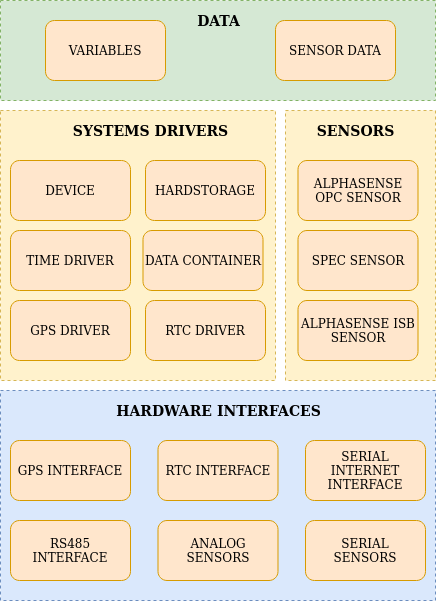
\includegraphics[width=0.75\linewidth]{chapters//2-CLEAN/Figuras/Diagrama de bibliotecas.png}
    \label{fig:fw-libraries-structure}
\end{figure}

\subsection{O módulo de interfaces de \textit{hardware}}

As Interfaces de \textit{Hardware} abrangem as funcionalidades relacionadas à comunicação e interface de sensores de gás, módulos de geoposicionamento (\acrshort{gps}) e relógio de tempo real (\acrshort{rtc}) que foram utilizados nos equipamentos desenvolvidos. O modo de operação e a saída dos sensores e de cada dispositivos de \textit{hardware} determinarão o seu esquema de conexão ao microcontrolador e a forma como sua leitura é implementada no \textit{firmware}.

A Figura \ref{fig:fw-libraries-hw-interfaces} mostra um diagrama das classes que foram implementadas para a versão atual do \textit{firmware}. As classes \texttt{SerialSensorInterface} e \texttt{AnalogSensorInterface} implementam interfaces para sensores digitais e analógicos, respectivamente. \texttt{SerialSensorInterface}, em particular, implementa uma interface para um sensor digital conectado através de um barramento \acrshort{uart} ou RS-485, por meio das classes filhas \texttt{UARTSensorInterface} e \texttt{RS485SensorInterface}. 

Cada classe implementa seu próprio método \texttt{sense()} que recebe como parâmetros um ponteiro para um objeto \texttt{Stream} (geralmente uma porta serial do microcontrolador), e um ponteiro para um \texttt{SerialParser}, que analisa as cadeias de caracteres com comandos ou dados enviados pelo sensor digital. O \texttt{SerialParser} é implementado numa camada superior pelas classes do módulo \texttt{Sensor}.

\begin{figure}[h]
    \centering
    \caption{Diagramas de classes do pacote \textit{Hardware} Interfaces}
    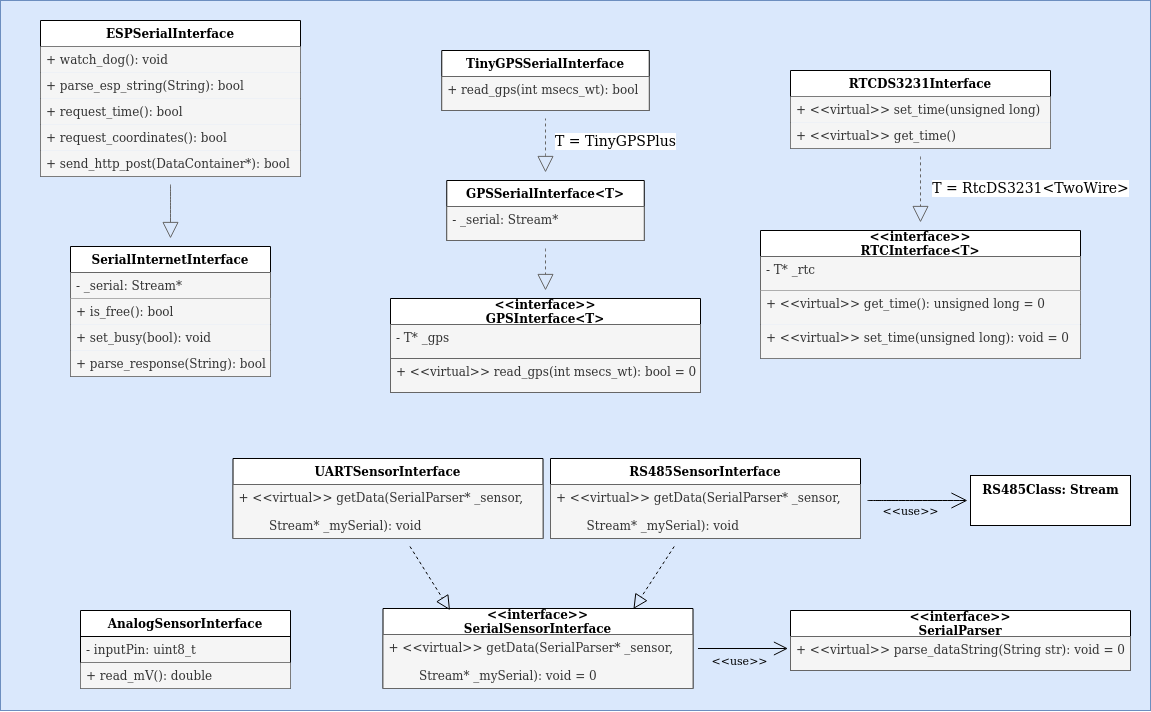
\includegraphics[width=0.90\linewidth]{chapters//2-CLEAN/Figuras/Diagrama-de-classes-Hardware-Interfaces.png}
    \label{fig:fw-libraries-hw-interfaces}
\end{figure}

A interface com um dispositivo serial para conexão à internet foi implementada através das classes \texttt{SerialInternetInterface} e \texttt{ESPSerialInterface}, esta última representando a conexão com o microcontrolador ESP8266. Foram criadas mais duas interfaces para módulos \acrshort{gps} e \acrshort{rtc}. Na versão atual do \texttt{firmware}, foram utilizadas as bibliotecas \texttt{TinyGPSPlus} e \texttt{RtcDS3221} para cada módulo respectivamente, porém, qualquer outra biblioteca ou módulo também pode ser usado, desde que seja criado como uma classe filha de \texttt{GPSSerialInterface} e \texttt{RTCInterface}. Para isso, as classes filhas deverão implementar os métodos virtuais: \texttt{readGPS()}, \texttt{set\_time()} e \texttt{get\_time()} respectivamente.

\subsection{O módulo \textit{drivers}}

Os \textit{Drivers} atuam como uma camada intermediária entre as Interfaces de \textit{Hardware} e o programa principal. Eles abstraem o \textit{hardware} dos dispositivos do código principal, permitindo sua reutilização independentemente dos módulos e bibliotecas utilizadas em um nível inferior. Alguns \textit{drivers} implementados para o \textit{firmware} foram:

\begin{itemize}
    \item O driver \texttt{HardStorage}, para armazenamento de dados em cartão \textit{SD}; 
    \item O \texttt{RTCDriver} para a Interface \acrshort{rtc};
    \item O \texttt{GPSDriver} para a Interface \acrshort{gps}; 
    \item O \texttt{TimeDriver} para gerenciamento das fontes de tempo no dispositivo, as quais podem provir de um módulo \acrshort{rtc}, um módulo \acrshort{gps} ou de um servidor \acrshort{ntp}
\end{itemize}

Esses quatro \textit{drivers} usam métodos estáticos, o que significa que podem ser usados sem necessidade de ter um objeto implementado no código. 

Os outros dois \textit{drivers} que foram implementados estão relacionados ao tratamento dos dados. São eles o \texttt{DataContainer} e o \texttt{Smoother}. A Figura \ref{fig:fw-libraries-drivers} mostra o diagrama de classes deste módulo. A continuação são resumidos alguns dos principais métodos e atributos de cada uma das classes pertencentes ao módulo \texttt{Drivers}.

\begin{figure}[h]
    \centering
    \caption{Diagrama de classes do Módulo \textit{Drivers}}
    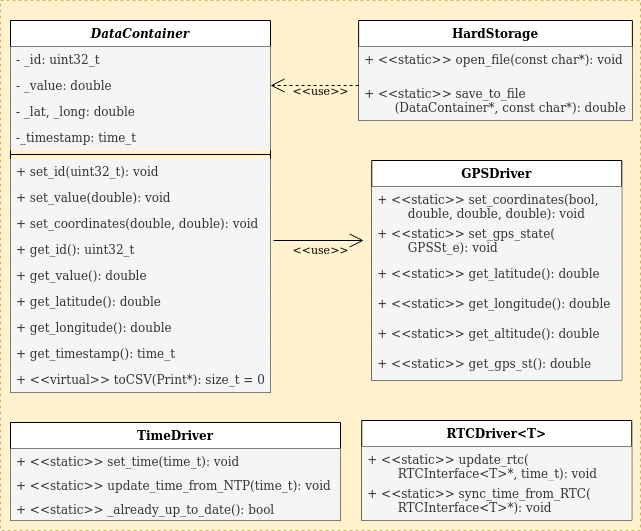
\includegraphics[width=0.90\linewidth]{chapters//2-CLEAN/Figuras/Diagrama-de-classes-System-Drivers-1.png}
    \label{fig:fw-libraries-drivers}
\end{figure}

\subsubsection{TimeDriver}
Esta classe registra a data e hora internas do sistema e fornece métodos para retornar informações de data e hora em diferentes formatos. O método \texttt{set\_time(time\_t)} define a data e hora do sistema. Internamente, ele invoca o método \texttt{setTime()} da biblioteca \texttt{Time.h} do framework Arduino. Recebe como parâmetro um número inteiro de 32 bits contendo a data e hora fornecidas por alguma fonte de relógio externa (um módulo \acrshort{gps}, um módulo \texttt{rtc} ou um servidor \texttt{ntp}).
\subsubsection{GPSDriver}
Esta classe controla a interface com um módulo \texttt{gps}, armazena as informações das coordenadas geográficas do sistema e fornece métodos para acessá-las, sendo eles:

\begin{itemize}
    \item \texttt{{static} get\_latitude(): double}
    \item \texttt{{static} get\_longitude(): double}
    \item \texttt{{static} get\_altitude(): double}
    \item \texttt{{static} get\_gps\_st(): GPSSt\_e}
\end{itemize}

Esses métodos fornecem as informações de geolocalização armazenadas no \texttt{GPSDriver}, bem como o estado dessas informações. As informações de geolocalização podem estar OK ou desatualizadas. Esses dois valores são retornados como uma enumeração do tipo \texttt{GPSSt\_e}.

Outros dois métodos definem as coordenadas geográficas do sistema e o estado dessa informação. Esses métodos são chamados por uma instância de GPSInterface. Eles são:

\begin{itemize}
    \item \texttt{{static} set\_coordinates(): void}
    \item \texttt{{static} set\_gps\_state(): void}
\end{itemize}

\subsubsection{RTCDriver}
Esta classe controla a interface com um módulo \acrshort{rtc}. O método \texttt{update\_rtc(RTCInterface*, time\_t)} é chamado sempre que o módulo \acrshort{rtc} precisa ser atualizado. Recebe como parâmetro um ponteiro para a instância do \texttt{RTCInterface} que será atualizada e a data e hora. O método \texttt{sync\_time\_from\_RTC(RTCInterface*)} retorna a data e hora a partir do ponteiro ao tipo \texttt{RTCInterface} passado como parâmetro

\subsubsection{DataContainer}
Esta é uma classe abstrata que contém informações sobre a leitura de uma variável. Essas informações são: o identificador da variável que está sendo medida e o valor dessa variável; as coordenadas; e a data e hora onde a valor foi medido. Objetos desta classe são usados para armazenar dados no cartão SD e para enviar postagens \textit{HTTP}. O método \texttt{toCSV(Print*)} é um método virtual puro para formatar os dados de uma leitura de variável e armazená-los em um arquivo \acrshort{csv}. Por se tratar de um método virtual, ele deve ser implementado pelas classes filhas de \texttt{DataContainer}. Desta forma cada aplicação pode ter seu próprio formato de armazenamento das informações.

\subsubsection{HardStorage}
Esta classe contém os métodos para leitura e gravação de e para um cartão SD. Para leitura, o método \texttt{open\_file(const char*)} abre o arquivo no qual as operações de leitura/gravação serão executadas. O método recebe o nome do arquivo como parâmetro. Já para a escrita no cartão, o método \texttt{save\_to\_file<T>(DataContainer*, const char*)} grava dados em um arquivo no cartão SD. O nome do arquivo é passado como parâmetro, juntamente com os dados a serem salvos. A função espera um ponteiro para um \texttt{DataContainer}, que na versão atual do \textit{firmware} são objetos do tipo \texttt{SensorData}. O objeto \texttt{SensorData} implementa o método \texttt{toCSV(Print*)}, que recebe um ponteiro para o arquivo e armazena os dados nele.

\subsection{O módulo Sensores}

As classes deste pacote encapsulam a lógica de leitura de cada sensor, considerando as especificações de cada fabricante. Eles fazem uso das interfaces de sensores implementadas no pacote de Interfaces de \textit{Hardware}. Dois fabricantes de sensores foram utilizados no \textit{hardware} dos equipamentos desenvolvidos no contexto deste trabalho: Alphasense e SPEC Sensors. As interfaces dos sensores Alphasense e SPEC diferem na forma como foram implementadas. As saídas dos sensores Alphasense são dois sinais de tensão analógicos. Os sensores SPEC, por outro lado, fornecem os valores de concentração de gás, temperatura e umidade em uma cadeia de caracteres que é enviada através de uma interface \acrshort{uart}. A Figura \ref{fig:fw-libraries-sensors} mostra um diagrama das classes implementadas para este módulo.

\begin{figure}[h]
    \centering
    \caption{Diagramas de classes do módulo Sensors}
    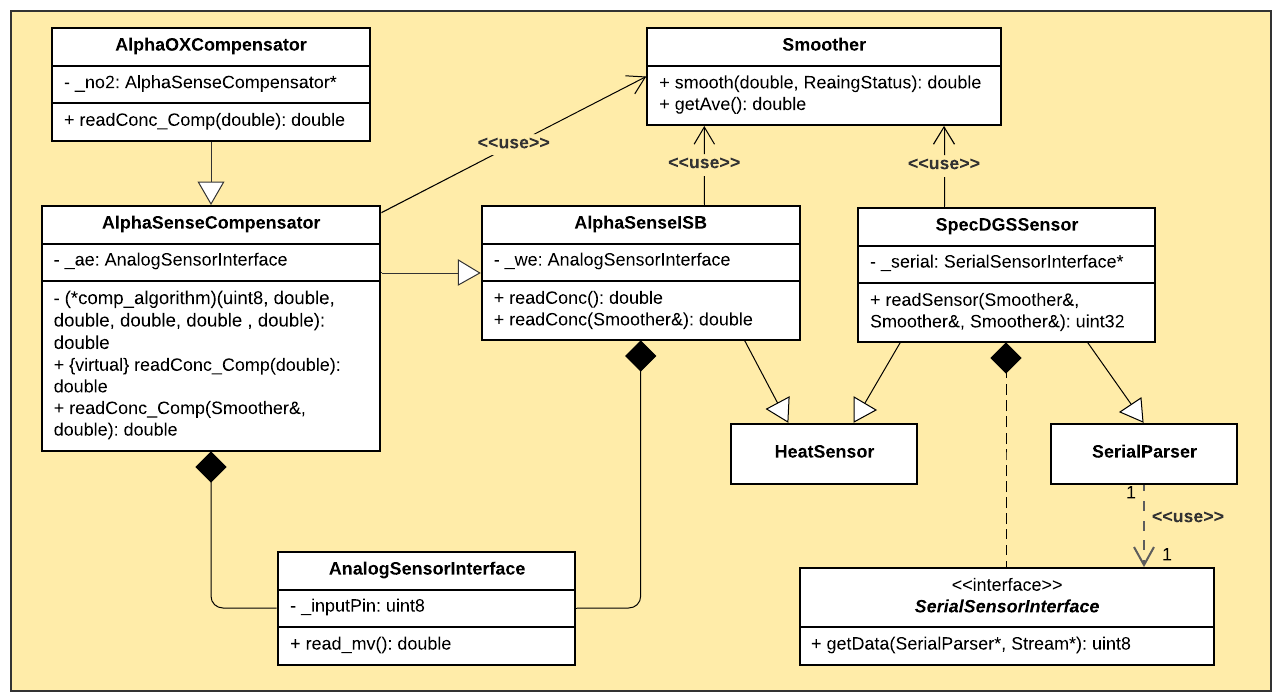
\includegraphics[width=0.90\linewidth]{chapters//2-CLEAN/Figuras/Diagrama-de-classes-Sensors-Package.png}
    \label{fig:fw-libraries-sensors}
\end{figure}

A base para o interfaceamento dos sensores Alphasense é a leitura de duas entradas analógicas do microcontrolador utilizando a função \texttt{analogRead()} do \textit{framework} Arduino. Por esse motivo, a classe base para modelagem dos sensores Alphasense é a classe \texttt{AnalogSensorInterface}. Ela representa uma entrada analógica identificada pelo atributo \texttt{\_inputPin}, e seu método \texttt{read\_mv()} converte o valor digital adquirido pelo conversor analógico-digital do Arduino, em um valor de tensão entre 0 – 5 V. Este método pode receber como parâmetro uma referência a um objeto do tipo \texttt{Smoother}, que por sua vez deve estar associado a um objeto \texttt{Variable}. Assim, são vinculadas as variáveis físicas modeladas no \textit{firmware} com a respectiva interface de \textit{hardware}; neste caso uma entrada analógica.

A classe \texttt{HeatSensor} representa um sensor que precisa de um tempo de aquecimento para funcionar. A lógica que determina a validade das leituras dos sensores é implementada dentro desta classe, levando em consideração um período de aquecimento para cada sensor. Do \texttt{HeatSensor} derivam as classes que representam os sensores Alphasense e SPEC, uma vez que ambos são sensores eletroquímicos amperométricos que requerem um intervalo de aquecimento para garantir que as leituras sejam válidas. A continuação resumem-se as principais propriedades das classes relacionadas ao interfaceamento dos sensores de gases.

\subsubsection{\texttt{AlphaSenseISB}}
Esta classe representa um sensor Alphasense com um circuito de condicionamento do tipo \acrshort{isb}. O sufixo "ISB" indica que o circuito de condicionamento usado é a placa de detecção individual do fabricante do sensor. Esta classe não incorpora nenhum algoritmo de compensação.

\textbf{Atributos:}
\texttt{\_we: AnalogSensorInterface}: Este é um atributo privado que representa a entrada analógica conectada ao eletrodo de trabalho (WE) do sensor

\textbf{Métodos:}
\texttt{readConc(): double}
\texttt{readConc(Smoother\&): double}
Estes são métodos públicos que convertem o valor de tensão lido pelo atributo \texttt{\_we} em um valor de concentração, levando em consideração a sensibilidade do sensor informada pelo fabricante. A referência ao objeto \texttt{Smoother} associa o sensor à variável física correspondente e retorna um valor suave das leituras da variável.

\subsubsection{\texttt{AlphaSenseCompensator}}
Derivado do \texttt{AlphaSenseISB}, representa um sensor Alphasense com um algoritmo de compensação. Os sensores da série Alphasense B4 podem usar diferentes algoritmos de compensação dependendo do gás ao qual são sensíveis. Por isso, cada algoritmo é inerente a cada objeto e não à classe

\textbf{Atributos:}
\texttt{\_ae: AnalogSensorInterface}: Este é um atributo privado que representa a saída do eletrodo auxiliar (AE) do sensor eletroquímico. O valor de saída deste eletrodo é usado nos algoritmos de compensação.

\textbf{Métodos:}
\texttt{(*comp\_algorithm)(uint8, double, double, double, double, double): double}: Este é um ponteiro para a função que implementa o algoritmo de compensação. As funções recebem como parâmetros as variáveis necessárias para o cálculo do algoritmo, dentre eles a temperatura.

\texttt{{virtual} readConc\_Comp(double): double}
\texttt{readConc\_Comp(Smoother\&, double): double}
Estes são métodos públicos que leem os valores de tensão armazenados nos atributos \texttt{\_we} (herdados do \texttt{AlphaSenseISB}) e \texttt{\_ae}. Eles aplicam o algoritmo de compensação correspondente e retornam um valor de concentração. Ambos os métodos recebem como parâmetros a temperatura ambiente e uma referência a um objeto \texttt{Smoother}, como no \texttt{AlphaSenseISB}.

\subsubsection{\texttt{AlphaOXCompensator}}
Este é um caso especial para sensores de ozônio que utilizam um algoritmo de compensação. Os sensores de ozônio medem, na verdade, a soma das concentrações de ozônio e dióxido de nitrogênio, portanto, o valor da concentração de dióxido de nitrogênio é exigido pelo algoritmo de compensação.

\textbf{Atributos:}
\texttt{\_no2: AlphaSenseCompensator*}: Para acessar o sensor de dióxido de nitrogênio, a classe \texttt{AlphaOXCompensator} usa um ponteiro para um objeto \texttt{AlphaSenseCompensator} que representa o sensor de dióxido de nitrogênio.

\textbf{Métodos:}
\texttt{readConc\_Comp(double): double}: Este método lê o valor da concentração do sensor de ozônio e aplica um algoritmo de compensação considerando também a concentração de dióxido de nitrogênio. Para vincular essas leituras a um objeto do tipo \texttt{Variable}, a classe \texttt{AlphaOXCompensator} utiliza o mesmo método \texttt{readConc\_Comp()} herdado da classe \texttt{AlphaSenseCompensator}, que recebe uma referência a um objeto do tipo \texttt{Smoother}.

\subsubsection{Interface com sensores seriais}

A interface com os sensores SPEC é realizada através da classe abstrata \texttt{SerialSensorInterface}. Esta classe fornece métodos para a leitura dos sensores através da porta serial do microcontrolador. A comunicação entre os sensores e o Arduino pode ser implementada através de uma interface \acrshort{uart} ou através de um barramento RS-485. Ambas as interfaces de comunicação são modeladas nas classes \texttt{UARTSensorInterface} e \texttt{RS485SensorInterface}, que derivam de \texttt{SerialSensorInterface}.

A classe \texttt{specDGS\_sensor} funciona como uma camada intermediária entre a interface de \textit{hardware} e as classes do módulo \texttt{Data}. Por representar um sensor eletroquímico que necessita de um período de aquecimento, esta classe também herda da classe \texttt{HeatSensor}. As instâncias de \texttt{specDGS\_sensor} têm a finalidade de ler e analisar as cadeias de caracteres enviadas pelos sensores SPEC, com as medições de temperatura, umidade e concentração de gás. Esta classe também é responsável por validar as medições levando em consideração o tempo de aquecimento dos sensores e possíveis erros na comunicação serial. O método \texttt{readSensor()} lê os valores de concentração, temperatura e umidade e os disponibiliza aos objetos de tipo \texttt{Variable} correspondentes por meio das referências \texttt{Smoother} que recebe como parâmetros.

O atributo \texttt{\_serial} da classe \texttt{specDGS\_sensor} é um ponteiro para um objeto do tipo \texttt{SerialSensorInterface}, que é atribuído durante a construção de cada instância \texttt{specDGS\_sensor}. O ponteiro pode ser um objeto do tipo \texttt{UARTSensorInterface} ou \texttt{RS485SensorInterface}, dependendo apenas da interface de comunicação implementada no \textit{hardware}. Os objetos \texttt{specDGS\_sensor} representam os sensores SPEC, e as instâncias derivadas da classe abstrata \texttt{SerialSensorInterface} representam a interface com esses sensores, que no \textit{hardware} é uma única porta serial.

\subsection{O módulo \texttt{Data}}

A Figura \ref{fig:fw-libraries-data} mostra o diagrama de classes do módulo \texttt{Data}. Como já mencionado, este módulo funciona como uma camada intermediária que prepara e formata as medições obtidas no \textit{hardware} do sensor para seu armazenamento e transmissão. É formado por duas classes principais: \texttt{Variable} e \texttt{SensorData}.

A classe \texttt{SensorData} método prepara os dados para transmissão remota e armazenamento local. Cada objeto do \texttt{SensorData} está associado a um único objeto do tipo \texttt{Variable}, que representa uma variável física com um identificador único. Vale ressaltar que, embora no \textit{firmware} cada variável física seja representada por um único identificador, no \textit{hardware} uma ou mais dessas variáveis podem estar vinculadas a um mesmo transdutor. O número de identificação que representa cada variável física é o que associa cada objeto da classe \texttt{Variable} ao objeto do tipo \texttt{SensorData} correspondente. Este número é armazenado em cada classe nos atributos \texttt{\_sensorID} e \texttt{\_id} como valores inteiros de 32 bits.

\begin{figure}[h]
    \centering
    \caption{Diagrama de classes do pacote \texttt{Data}}
    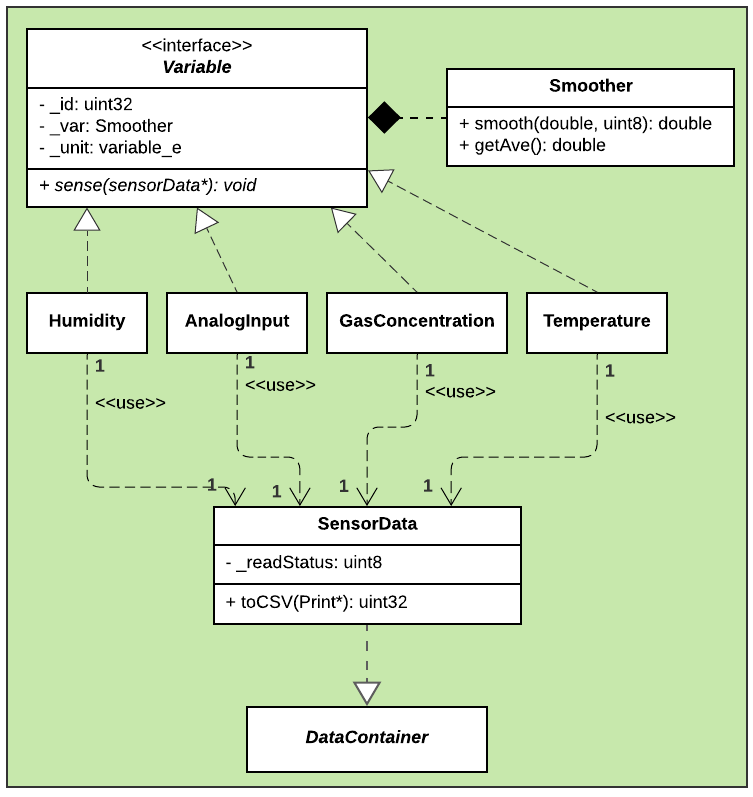
\includegraphics[width=0.80\linewidth]{chapters//2-CLEAN/Figuras/Diagrama-de-classes-Data-Package.png}
    \label{fig:fw-libraries-data}
\end{figure}

Objetos do tipo \texttt{SensorData} contêm o valor das variáveis físicas às quais estão associados, juntamente com informações sobre a data, hora e local onde as medições foram feitas. O valor de cada variável é armazenado no atributo \texttt{\_value}, o qual pode ser um dado bruto medido em determinado instante de tempo ou uma média de valores adquiridos durante uma janela temporal. O método \texttt{toCSV()} consolida e prepara as informações do valor medido pelo sensor, sua geolocalização, e a data e hora em que a medição foi realizada, no formato \acrshort{csv}.

A classe \texttt{Variable} atua como uma camada intermediária entre a camada de \textit{hardware} do sensor e a classe \texttt{SensorData}. Os objetos desta classe representam as variáveis físicas que estão sendo monitoradas, porém, não contêm suas quantidades, pois esses valores estão armazenados em objetos do tipo \texttt{SensorData}. Como já mencionado, o atributo \texttt{\_id} contém o identificador da variável física que representa. O atributo \texttt{\_unit} representa a unidade de medida da variável física que está sendo monitorada. O atributo \texttt{\_var}, do tipo \texttt{Smoother}, funciona como um buffer de memória no qual os objetos que implementam a interface de \textit{hardware} dos sensores podem colocar as amostras da variável medida. Desse mesmo buffer, o objeto \texttt{SensorData} associado pode extrair o valor médio das amostras. O número de amostras de cada buffer depende da capacidade que for programada. Os diagramas nas Figuras \ref{fig:fw-read-write-smoother} e\ref{fig:fw-sense-seq} ilustram este processo.

\begin{figure}[t]
    \centering
    \caption{Processo de leitura de uma variável}
    \begin{subfigure}{0.495\textwidth}
        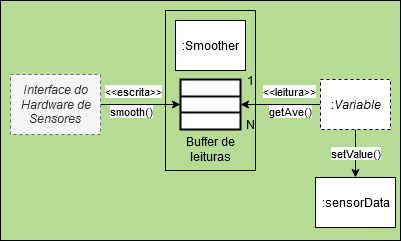
\includegraphics[width=\textwidth]{chapters/2-CLEAN/Figuras/Diagrama R_W Buffer Smoother.png}
        \caption{Processo de escrita e leitura no buffer da classe \textit{Smoother}}
        \label{fig:fw-read-write-smoother}
    \end{subfigure}
    \hfill
    \begin{subfigure}{0.495\textwidth}
        \includegraphics[width=\textwidth]{chapters/2-CLEAN/Figuras/Diagramas de sequências.png}
        \caption{Diagrama de sequências do método \textit{sense()}}
        \label{fig:fw-sense-seq}
    \end{subfigure}
    \hfill
    \label{fig:fw-read-variable}
    \fonte{Desenvolvido pelo autor (2023)}
\end{figure}

Os objetos que representam os sensores, gravam as leituras de cada variável física no buffer de amostragem através do método \texttt{smooth()} da classe \texttt{Smoother} (\ref{fig:fw-read-write-smoother}). Já a classe \texttt{Variable} acessa a média das amostras invocando o método \texttt{getAve()} do atributo \texttt{\_var}. Esse valor médio é transferido para o objeto \texttt{SensorData} associado por meio do método \texttt{setValue()}. O processo de leitura e transferência do valor médio das amostras para o objeto \texttt{SensorData} acontece dentro do método \texttt{sense()} definido na classe \texttt{Variable}. A Figura \ref{fig:fw-sense-seq} mostra o diagrama de sequência para este método.

A função \texttt{sense()} é um método virtual puro, portanto, as instâncias que derivam da classe abstrata \texttt{Variable} devem implementá-la. A sequência principal de ações executadas pelo método é comum a todas as classes derivadas. Quando o método \texttt{sense()} é invocado, a classe filha de \texttt{Variable} acessa, através do método \texttt{getAve()} de \texttt{Smoother}, o valor médio das amostras. Este valor é então passado para o objeto do tipo \texttt{SensorData} associado através do método \texttt{setValue()}. O objeto do tipo \texttt{SensorData}, por sua parte, armazena a data, a hora e o local onde foi feita a medição, bem como o status da leitura (método \texttt{getReadSt()}).

Os tipos de variáveis físicas implementadas na versão atual do \textit{firmware} foram: Temperatura, Umidade, Concentração de gás e Entrada Analógica. Esta última representa uma tensão analógica que pode ser lida como um sinal de tensão entre 0 – 5 V. Essas variáveis foram modeladas em classes filhas de \texttt{Variable} como \texttt{Temperature}, \texttt{Humidity}, \texttt{GasConcentration} e \texttt{AnalogInput}. Por serem classes filhas, todas possuem os mesmos atributos de \texttt{Variable}, mas cada uma implementa seu próprio método \texttt{sense()}.

% ----------------------------------------------------------
\section{A API Renovar}
% ----------------------------------------------------------

Renovar é uma plataforma Web que fornece dados de sensores de ar para visualização e uma \acrshort{api} para integração de sensores de ar \acrshort{iot}. Um \acrshort{mvp} da plataforma foi desenvolvido em parceria com o Departamento de Informática e Estatística da UFSC \cite{Teixeira2018} e foi continuado no \acrshort{lcqar} nos anos seguintes. A plataforma é composta por um banco de dados, um serviço de \textit{back-end} – desenvolvido em linguagem Java utilizando Spring Boot –, e uma aplicação \textit{front-end} criada em Angular, com Ionic e TypeScript. Seu acesso é gratuito e aberto para pesquisas e análises ambientais. A Figura \ref{fig:renovar-map} ilustra o painel principal da plataforma, o qual consiste em um mapa que mostra a localização dos dispositivos de monitoramento. A Figura \ref{fig:renovar-series} ilustra o painel de séries temporais, onde o usuário consegue visualizar o histórico de determinada variável num intervalo de tempo selecionável.

\begin{figure}[h]
    \centering
    \caption{Aplicação web Renovar}
    \begin{subfigure}{0.495\textwidth}
        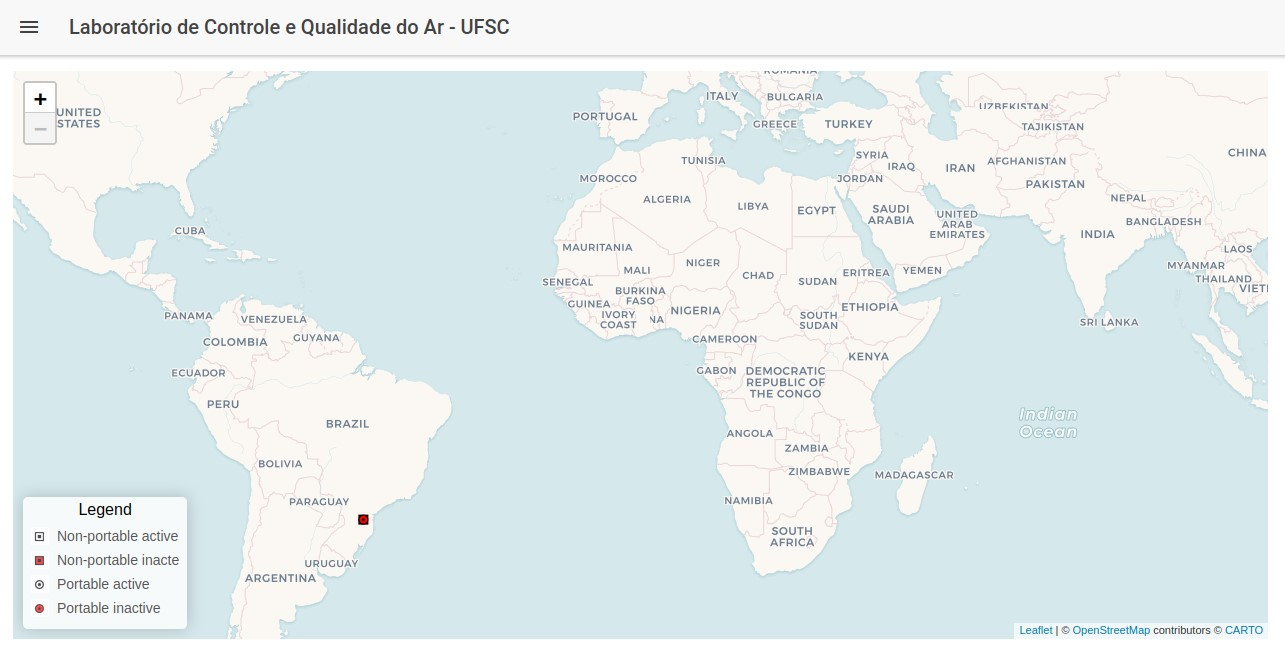
\includegraphics[width=\textwidth]{chapters/2-CLEAN/Figuras/Renovar main panel.jpeg}
        \caption{Painel principal}
        \label{fig:renovar-map}
    \end{subfigure}
    \hfill
    \begin{subfigure}{0.495\textwidth}
        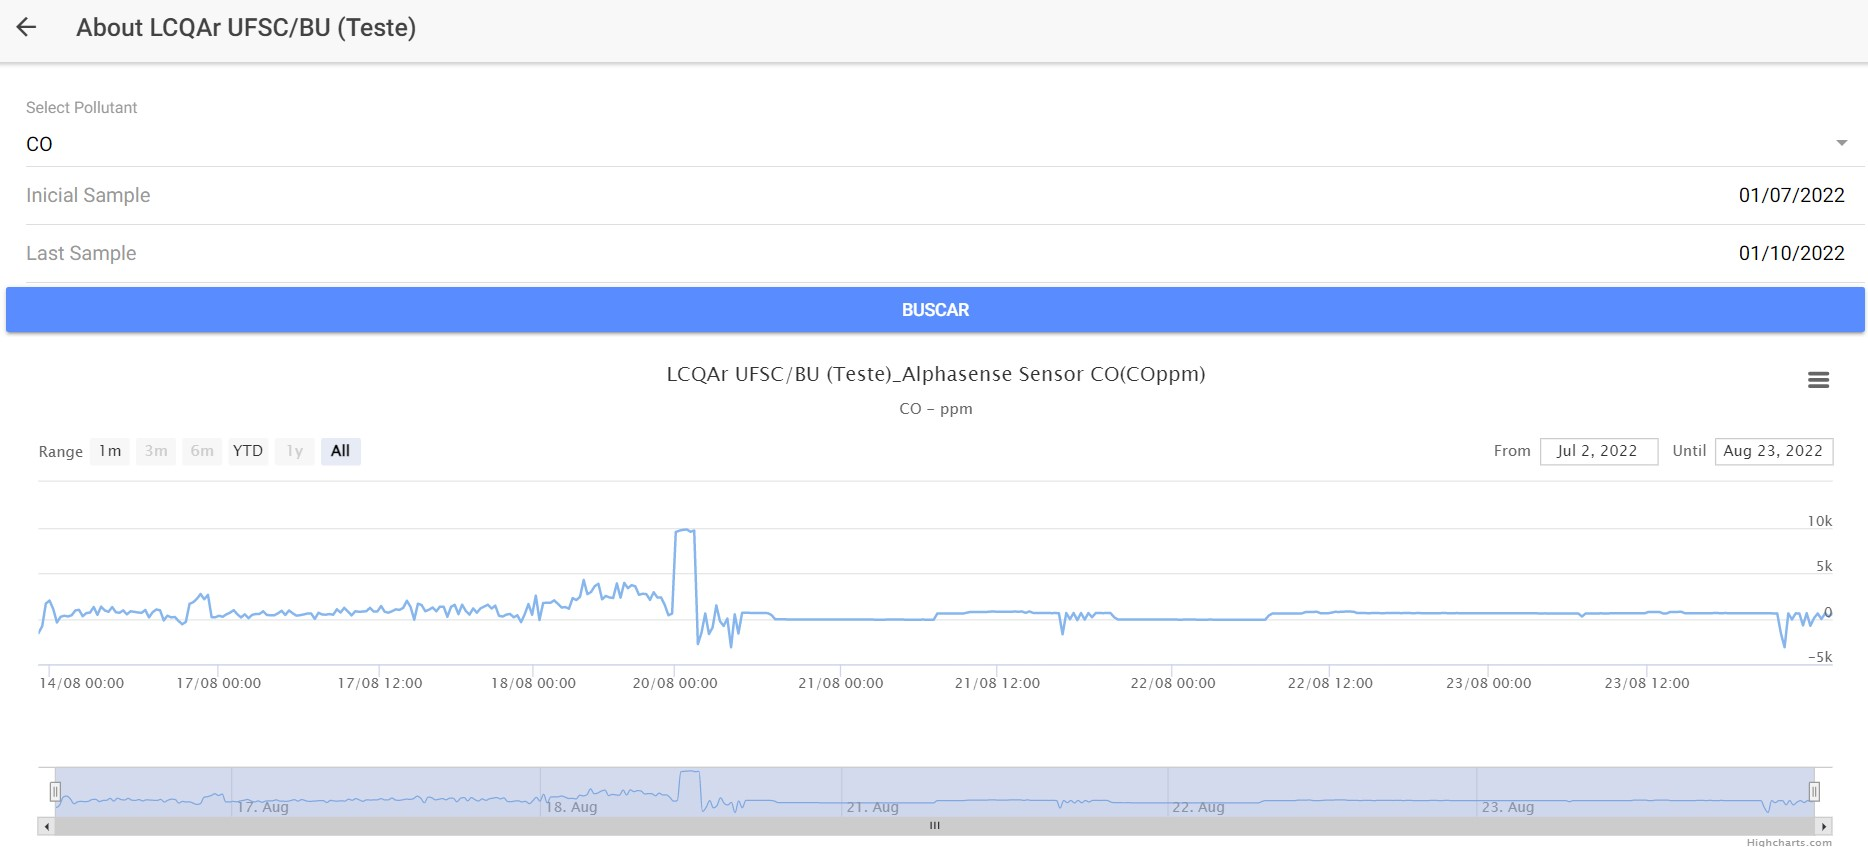
\includegraphics[width=\textwidth]{chapters/2-CLEAN/Figuras/ Renovar time series panel.jpg}
        \caption{Painel de visualização de séries temporais}
        \label{fig:renovar-series}
    \end{subfigure}
    \hfill
    \label{fig:renovar-map-and-series}
    \fonte{Desenvolvido pelo autor (2023)}
\end{figure}

O sistema recebe dados de dispositivos \acrshort{iot}, como concentração de poluentes atmosféricos, temperatura e umidade relativa. Os dados são armazenados em um banco de dados como séries temporais que podem ser visualizadas online na plataforma \textit{web}. O software consiste em (1) um banco de dados MySQL que armazena as leituras do dispositivo e demais dados necessários à plataforma, como usuários, dispositivos cadastrados, poluentes e unidades; (2) um back-end RESTful, desenvolvido em Java utilizando Spring Boot, que é responsável por coletar dados do banco de dados e prepará-los para o frontend; e (3) o front-end, desenvolvido para ser multiplataforma, disponibilizando a interface com o usuário conforme ilustrado nas imagens da Figura \ref{fig:renovar-map-and-series}. O banco de dados, backend e frontend estão hospedados em um servidor da Universidade Federal de Santa Catarina.

\begin{figure}[h]
    \centering
    \caption{Estrutura da aplicação \textit{Web} Renovar}
    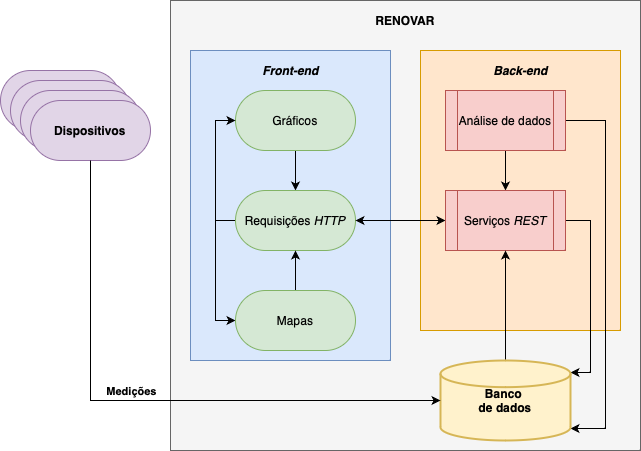
\includegraphics[width=0.80\linewidth]{chapters//2-CLEAN/Figuras/Renovar Structure (PT).png}
    \label{fig:renovar-structure}
    \fonte{Desenvolvido pelo autor (2023)}
\end{figure}

A Figura \ref{fig:renovar-structure} ilustra o funcionamento do serviço em geral. Os dispositivos coletam dados ambientais e os enviam para o banco de dados pela internet. O backend recebe solicitações do frontend e coleta os dados necessários do banco de dados. Caso os dados necessitem de algum tratamento (ex.: cálculo de valores médios ou filtragem), o backend executa as operações necessárias e envia as informações processadas de volta ao frontend. O frontend, por outro lado, implementa a interface com o usuário e gera os resultados das operações solicitadas, como visualizar os dados como séries temporais e baixar os dados como arquivo \acrshort{csv}.

\subsection{Banco de dados}

O banco de dados foi construído utilizando \textit{MySQL} como linguagem de consulta e \textit{phpMyAdmin} para administração. A Figura \ref{fig:renovar-database} ilustra a estrutura do banco, que consiste em oito entidades, cada uma com a sua função, atributos e relacionamentos. Elas são as entidades \textit{User}, \textit{Device}, \textit{Sensor}, \textit{Sample}, \textit{Coordinates}, \textit{Pollutant}, \textit{Unit} e \textit{Type}.

\begin{figure}[h]
    \centering
    \caption{Entidades do banco de dados Renovar}
    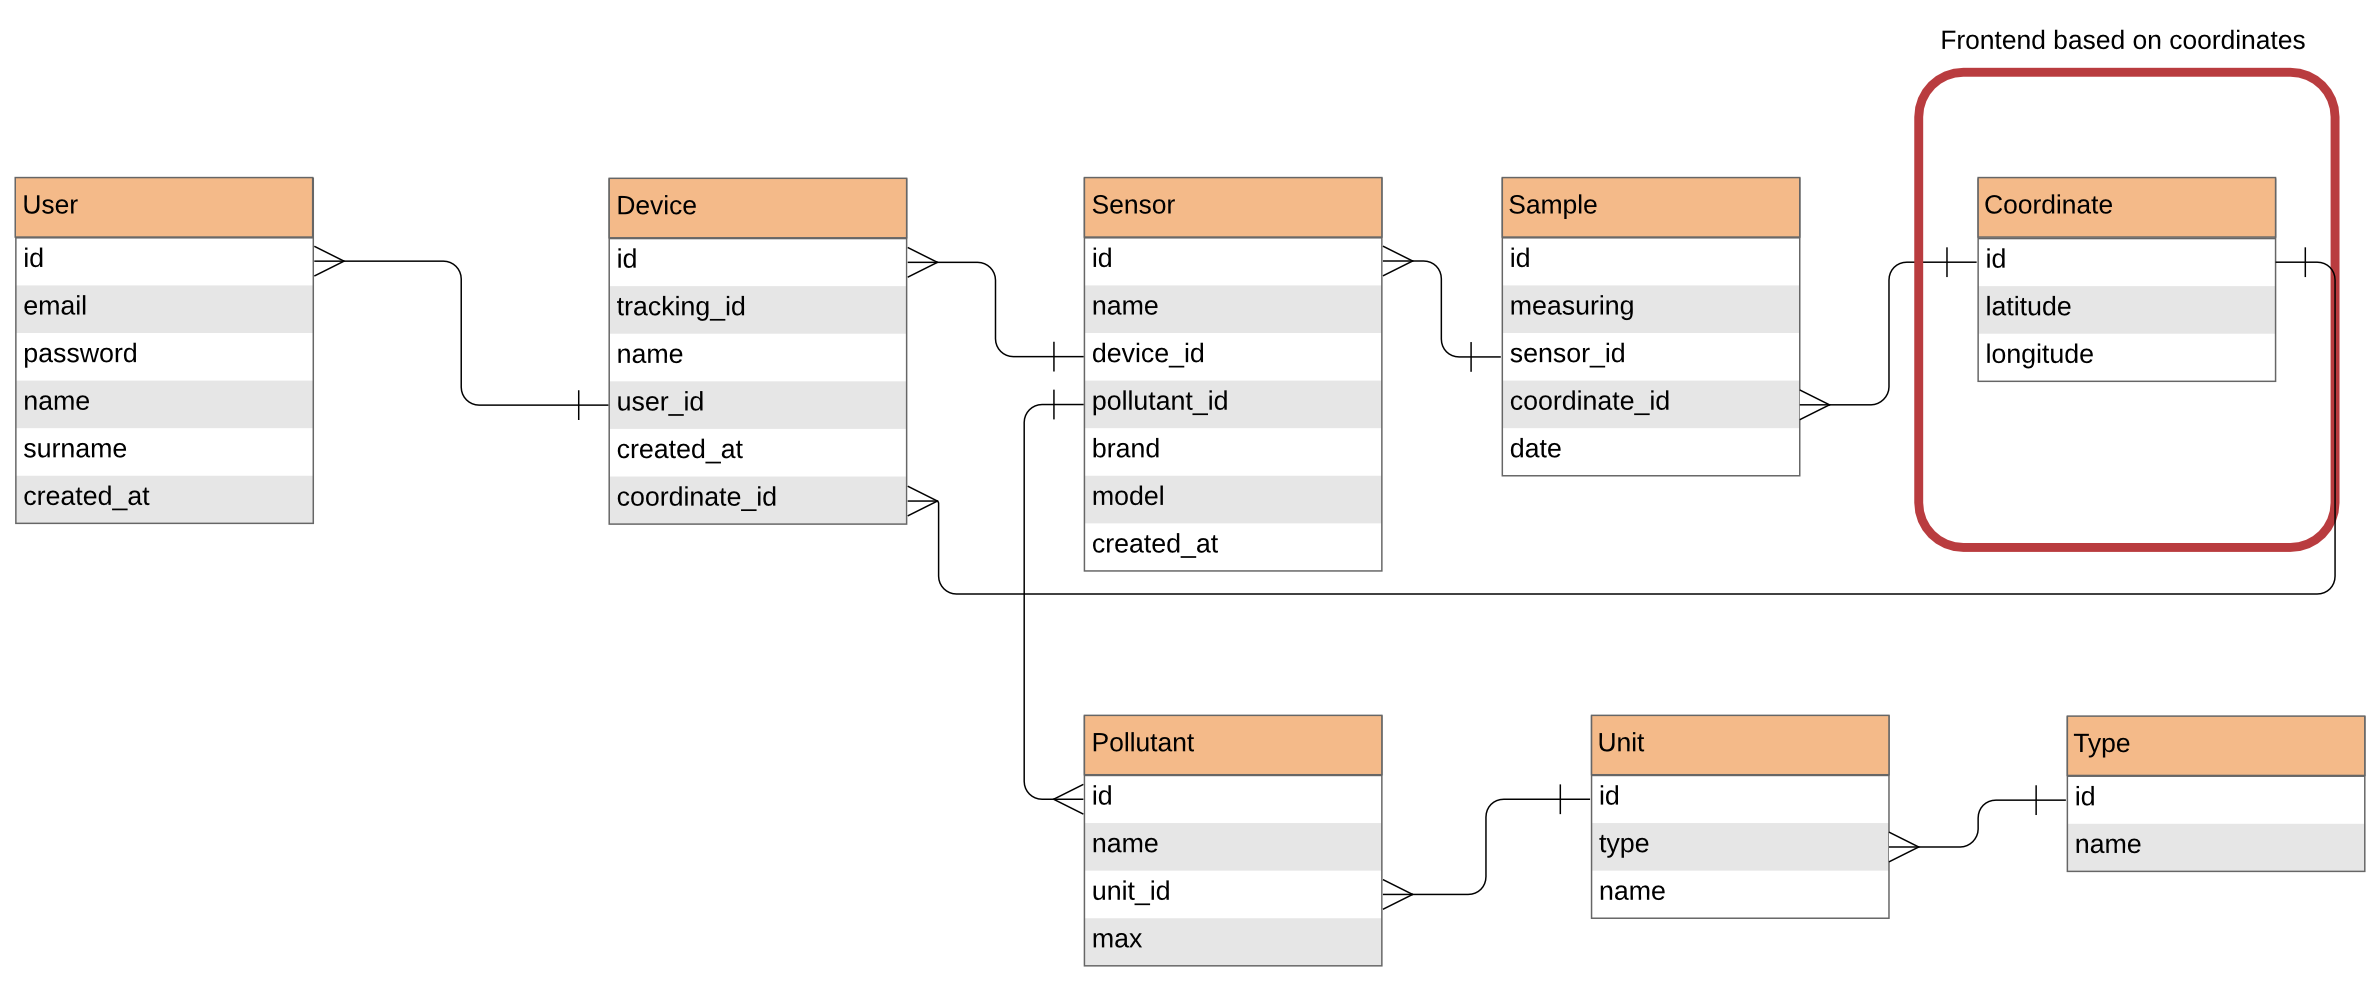
\includegraphics[width=0.80\linewidth]{chapters//2-CLEAN/Figuras/Renovar Database.png}
    \label{fig:renovar-database}
    \fonte{Desenvolvido pelo autor (2023)}
\end{figure}

A entidade \textit{Device} representa na prática os dispositivos de coleta, mais especificamente os monitores de qualidade do ar. A entidade \textit{Sensor} representa um sensor de determinada variável física. Relaciona-se com a entidade \textit{Device} com uma cardinalidade 1:N, ou seja, um dispositivo pode ter N sensores enquanto um sensor pode pertencer apenas a um dispositivo. \textit{Pollutant} representa as variáveis que são monitoradas no meio ambiente pelos dispositivos \acrshort{iot}. A relação entre \textit{Pollutant} e \textit{Sensor} também está caracterizada por uma cardinalidade 1:N, já que um sensor possui um único poluente, mas um mesmo poluente pode estar associado a N sensores. Cada poluente tem associado também uma unidade de medida e um tipo de unidade. A entidade \textit{Sample} representa uma leitura de determinada variável física; existem N amostras por sensor. Cada amostra tem associada uma coordenada, que é a localização geográfica onde o valor da amostra será mostrado no mapa. Os dispositivos para medição em locais fixos também tem associados uma Coordenada e consequentemente, todas as amostras dos sensores desse dispositivo devem possuir os mesmos valores de latitude e longitude. Por último, a entidade \textit{User} é utilizada para controle de acesso à plataforma. Embora o acesso aos dados de Renovar não precise de uma etapa de login, a escrita ou envio de dados para a plataforma precisa de um cadastro prévio. Assim, cada dispositivo deve ter um usuário associado para conseguir armazenar as leituras no banco de dados de Renovar.

\subsection{A aplicação \textit{Back-end}}

O backend é uma aplicação autônoma construída na linguagem de programação \textit{Java}, com o \textit{framework Spring Boot} e a ferramenta \textit{Maven}. Esta aplicação é responsável por receber e organizar as leituras enviadas pelos dispositivos \acrshort{iot}, no banco de dados e atender as requisições \textit{HTTP} do lado do cliente (\textit{front-end}). Igualmente a aplicação realiza algumas operações básicas de análise de dados como filtragem e agrupação para gráficos tipo \textit{box-plots}.

Quatro camadas compõem a aplicação: os controladores \acrshort{rest}, a camada de serviço, a camada de acesso aos dados e a camada de domínio (Figura \ref{fig:renovar-backend}) \cite{Teixeira2018}. São os controladores os que estabelecem os \textit{endpoints}, mensagens, conteúdos e cabeçalhos de cada recurso do \textit{back-end}. A Camada de Serviço está abaixo dos controladores \acrshort{rest} e funciona como um mediador entre a Camada de Acesso aos Dados e a Camada de Comunicação. É ela também quem define as regras de negócio da aplicação. A Camada de Domínio replica a modelagem do banco de dados em classes que são utilizadas pelos distintos componentes da aplicação; cada classe representa uma tabela. Por último a Camada de Acesso aos Dados tem a responsabilidade de acessar diretamente o banco de dados e disponibilizar a informação para as camadas superiores. A Figura \ref{fig:renovar-backend-dao} ilustra as classes utilizadas na Camada de Acesso aos Dados.

\begin{figure}[h]
    \centering
    \caption{Camadas da aplicação \textit{back-end} Renovar}
    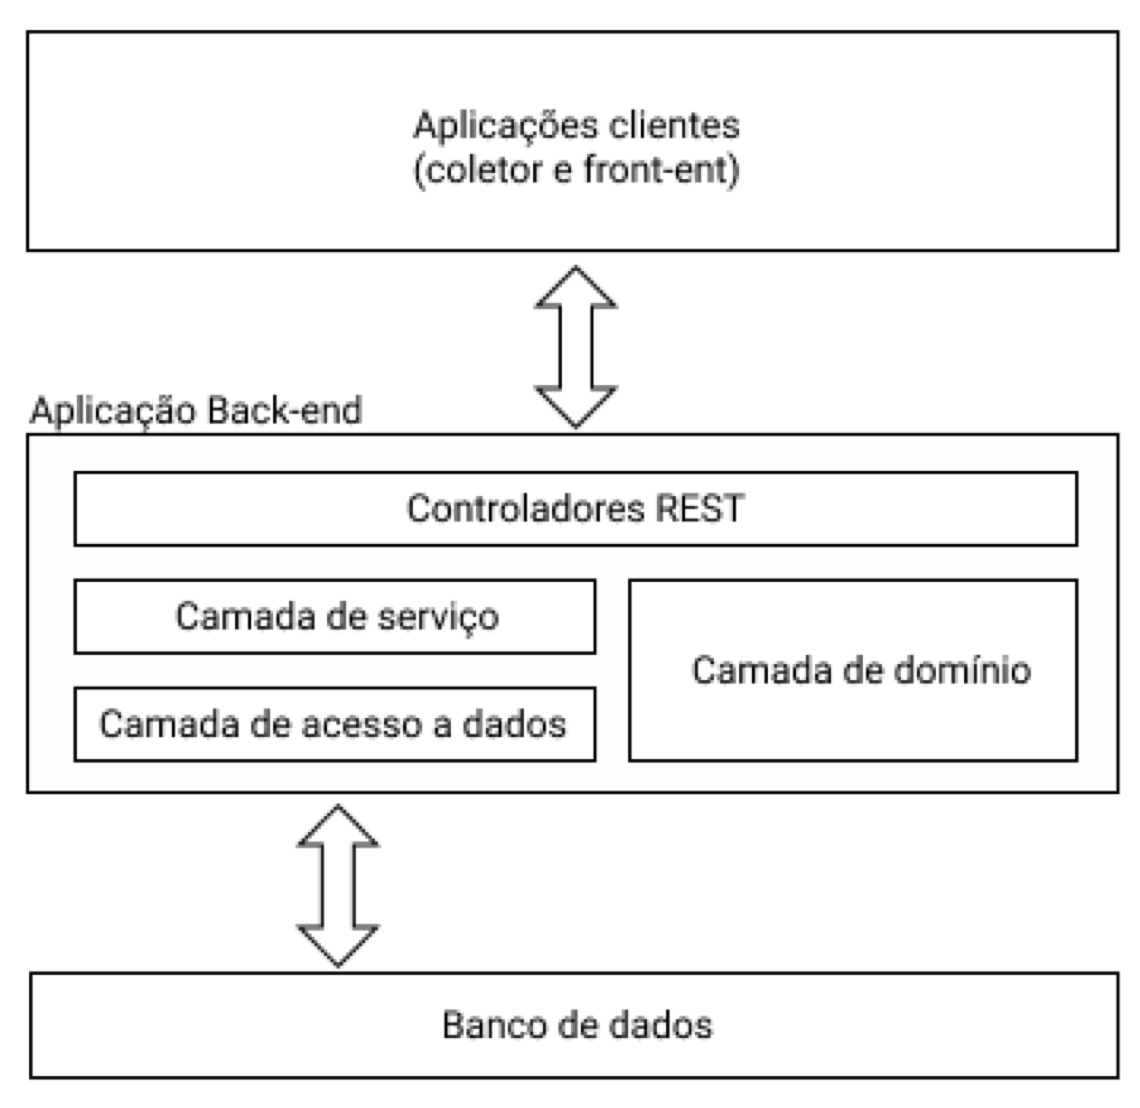
\includegraphics[width=0.80\linewidth]{chapters//2-CLEAN/Figuras/Renovar back-end strcuture.png}
    \label{fig:renovar-backend}
    \fonte{\cite{Teixeira2018}}
\end{figure}

\begin{figure}[h]
    \centering
    \caption{Classes de acesso ao dados da aplicação \textit{back-end} Renovar}
    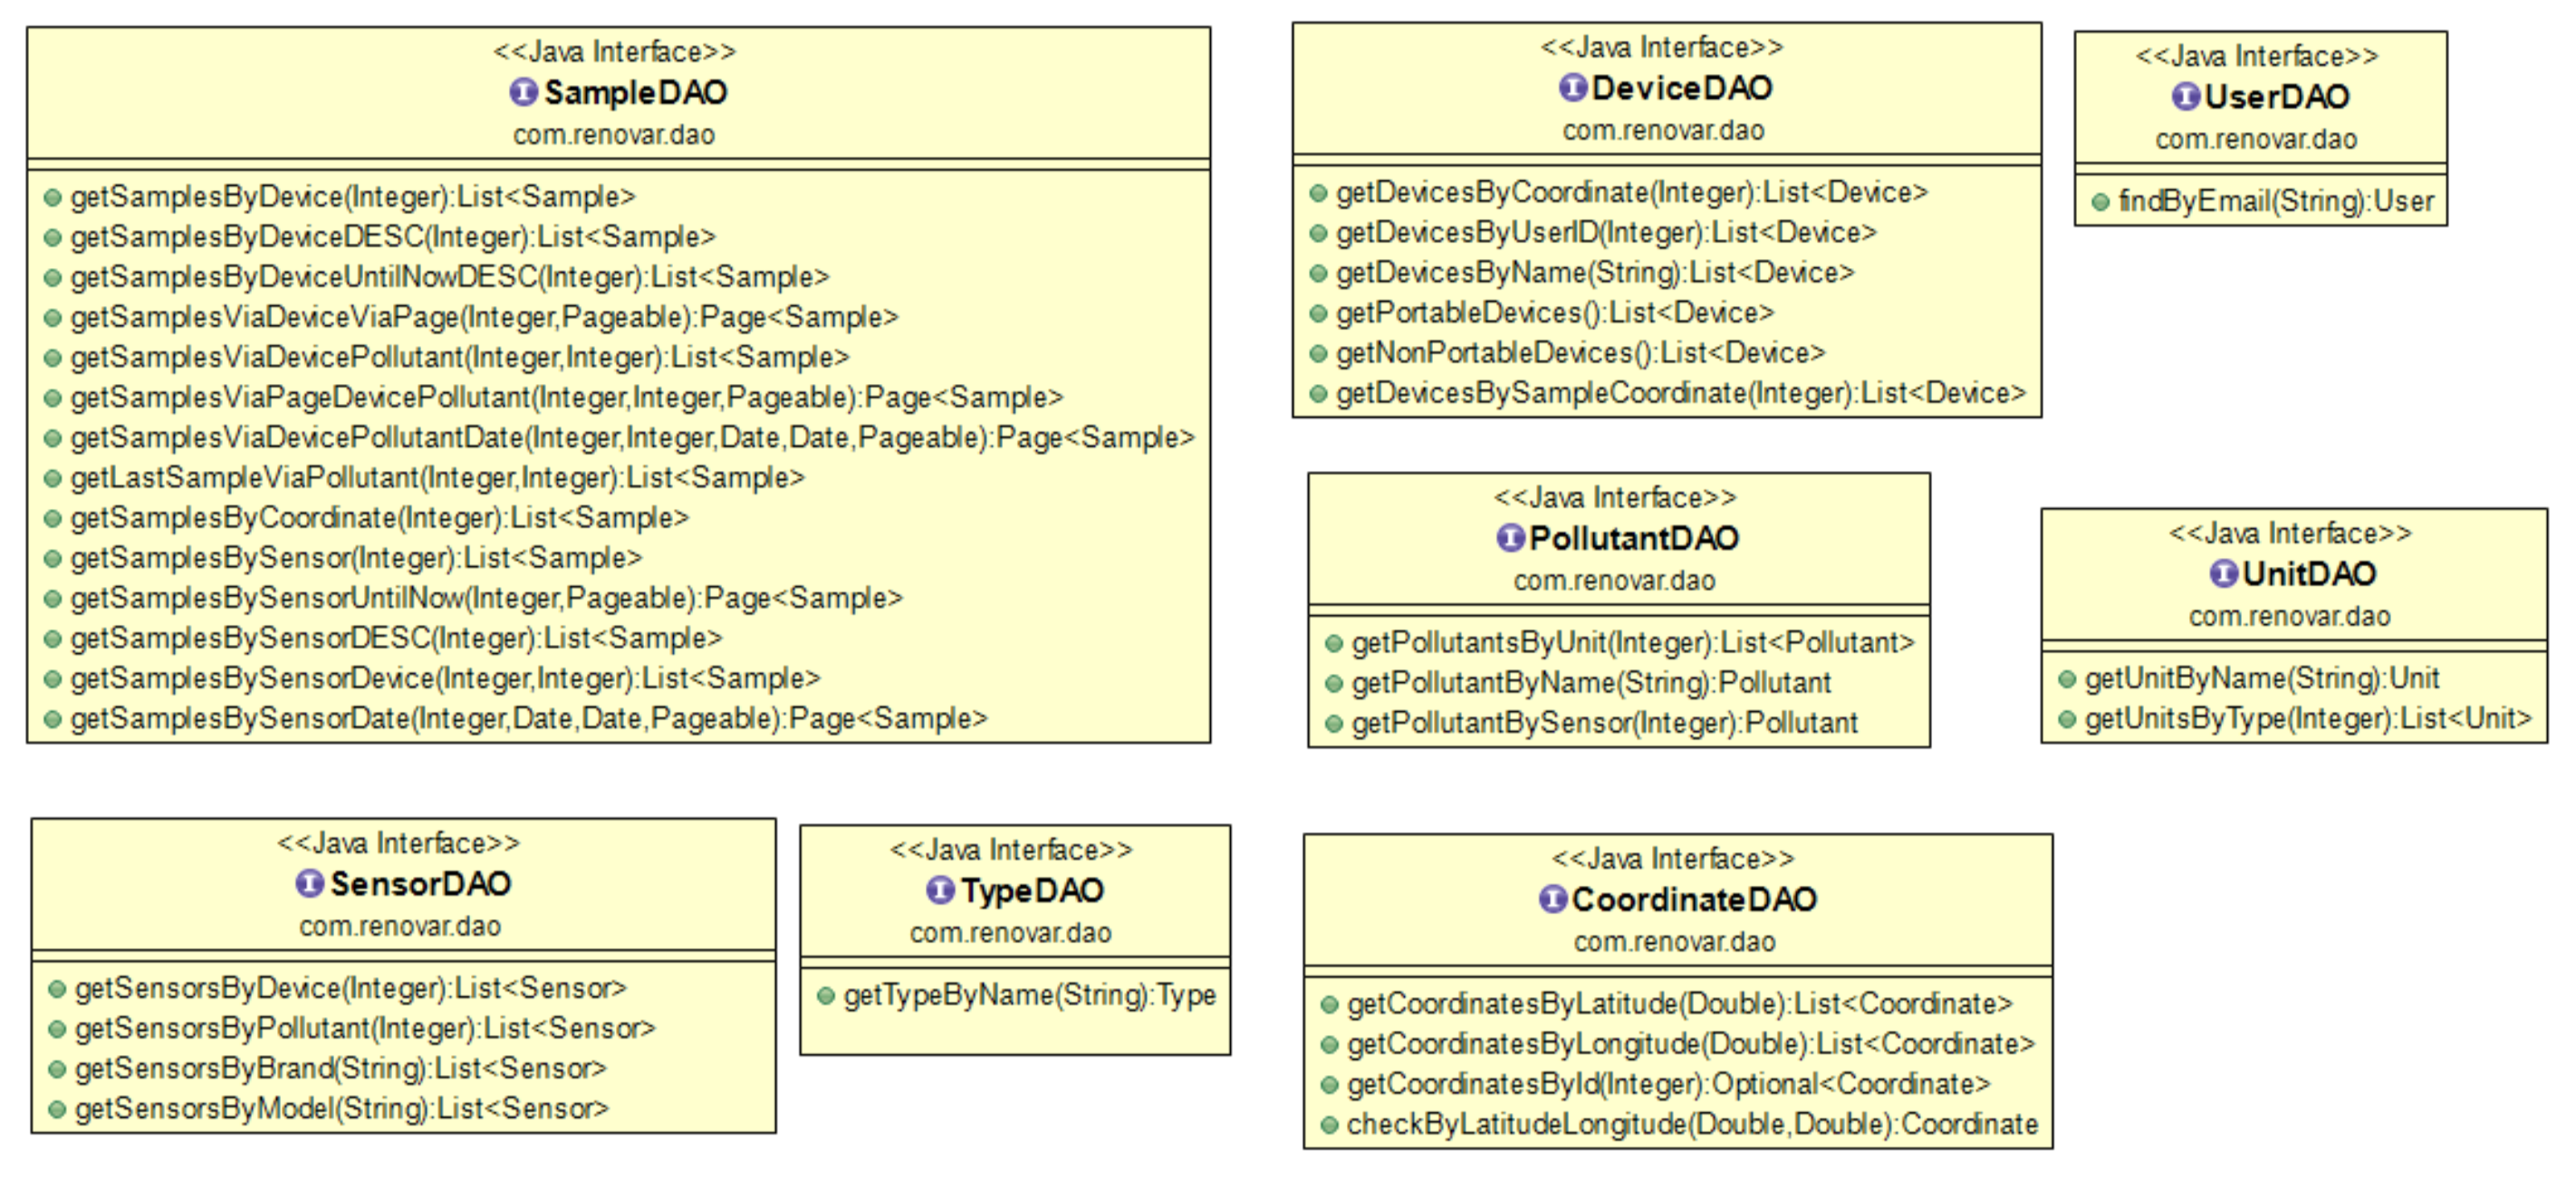
\includegraphics[width=0.80\linewidth]{chapters//2-CLEAN/Figuras/Classes de acesso aos Dados.png}
    \label{fig:renovar-backend-dao}
    \fonte{Desenvolvido pelo autor (2023)}
\end{figure}

O processo de coleta das medições enviadas pelos dispositivos de monitoramento na aplicação \textit{back-end} consiste, de forma simplificada, no seguinte fluxo de execução. Os controladores \acrshort{rest} processam as requisições de tipo \textit{POST HTTP} enviadas pelos dispositivos \acrshort{iot}, e transferem as informações até a camada de serviço. Ali os dados são validados e instâncias da entidade \textit{Sample} são criadas e transferidas até a camada de acesso aos dados onde as amostras são armazenadas na tabela correspondente do banco de dados. As requisições e os \textit{endpoints} disponibilizados na \acrshort{api} Renovar pelos controladores \acrshort{rest} são detalhados na documentação da \acrshort{api} disponibilizada no Anexo \ref{anex:renovar-api}.

\subsection{A aplicação \textit{Front-end}}

A aplicação \textit{front-end} foi construída usando o \textit{framework Angular}, junto com outras ferramentas como \textit{HighCharts} e \textit{HighStock} para os gráficos e \textit{Leaflet} para mapas. A tela principal mostra um mapa com todos os dispositivos (Figura \ref{fig:renovar-map-2}). A cor dos dispositivos no mapa indica seu estado: verde para ativo (i.e.: o dispositivo está transmitindo novas medidas), vermelho para inativo (o dispositivo não tem enviado novas medidas em um determinado intervalo de tempo). Quando o usuário seleciona um dispositivo no mapa, um \textit{pop-up} é aberto com informações sobre esse e todos os dispositivos que se encontrem nas mesmas coordenadas geográficas, juntamente com informações sobre seus sensores (Figura \ref{fig:renovar-devices}). A partir desse ponto, o usuário pode acessar a página do dispositivo e escolher um poluente para visualizar sua série histórica dentro de um intervalo de datas (Figura \ref{fig:renovar-series-2}). Se o aparelho for portátil, o usuário também pode ver outro mapa que mostra onde cada amostra foi coletada, conforme mostrado na Figura \ref{fig:renovar-portable-map}. Uma seção de análise de dados possibilita visualizar os valores das leituras dos sensores em gráficos de \textit{box-plots}, agrupando as medições por ano mês ou semana, conforme ilustra a Figura \ref{fig:renovar-data-analysis}.

\begin{figure}[h]
    \centering
    \caption{Aplicação \textit{front-end} da plataforma web Renovar}
    \begin{subfigure}{0.495\textwidth}
        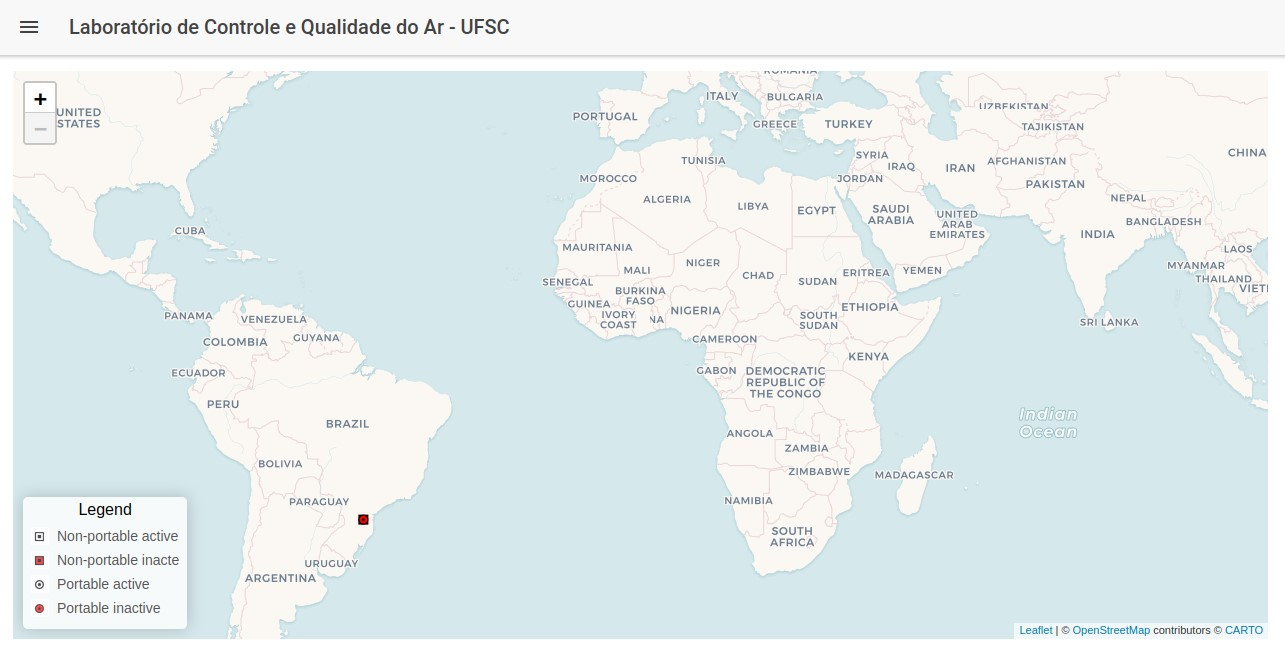
\includegraphics[width=\textwidth]{chapters/2-CLEAN/Figuras/Renovar main panel.jpeg}
        \caption{Mapa de dispositivos}
        \label{fig:renovar-map-2}
    \end{subfigure}
    \hfill
    \begin{subfigure}{0.495\textwidth}
        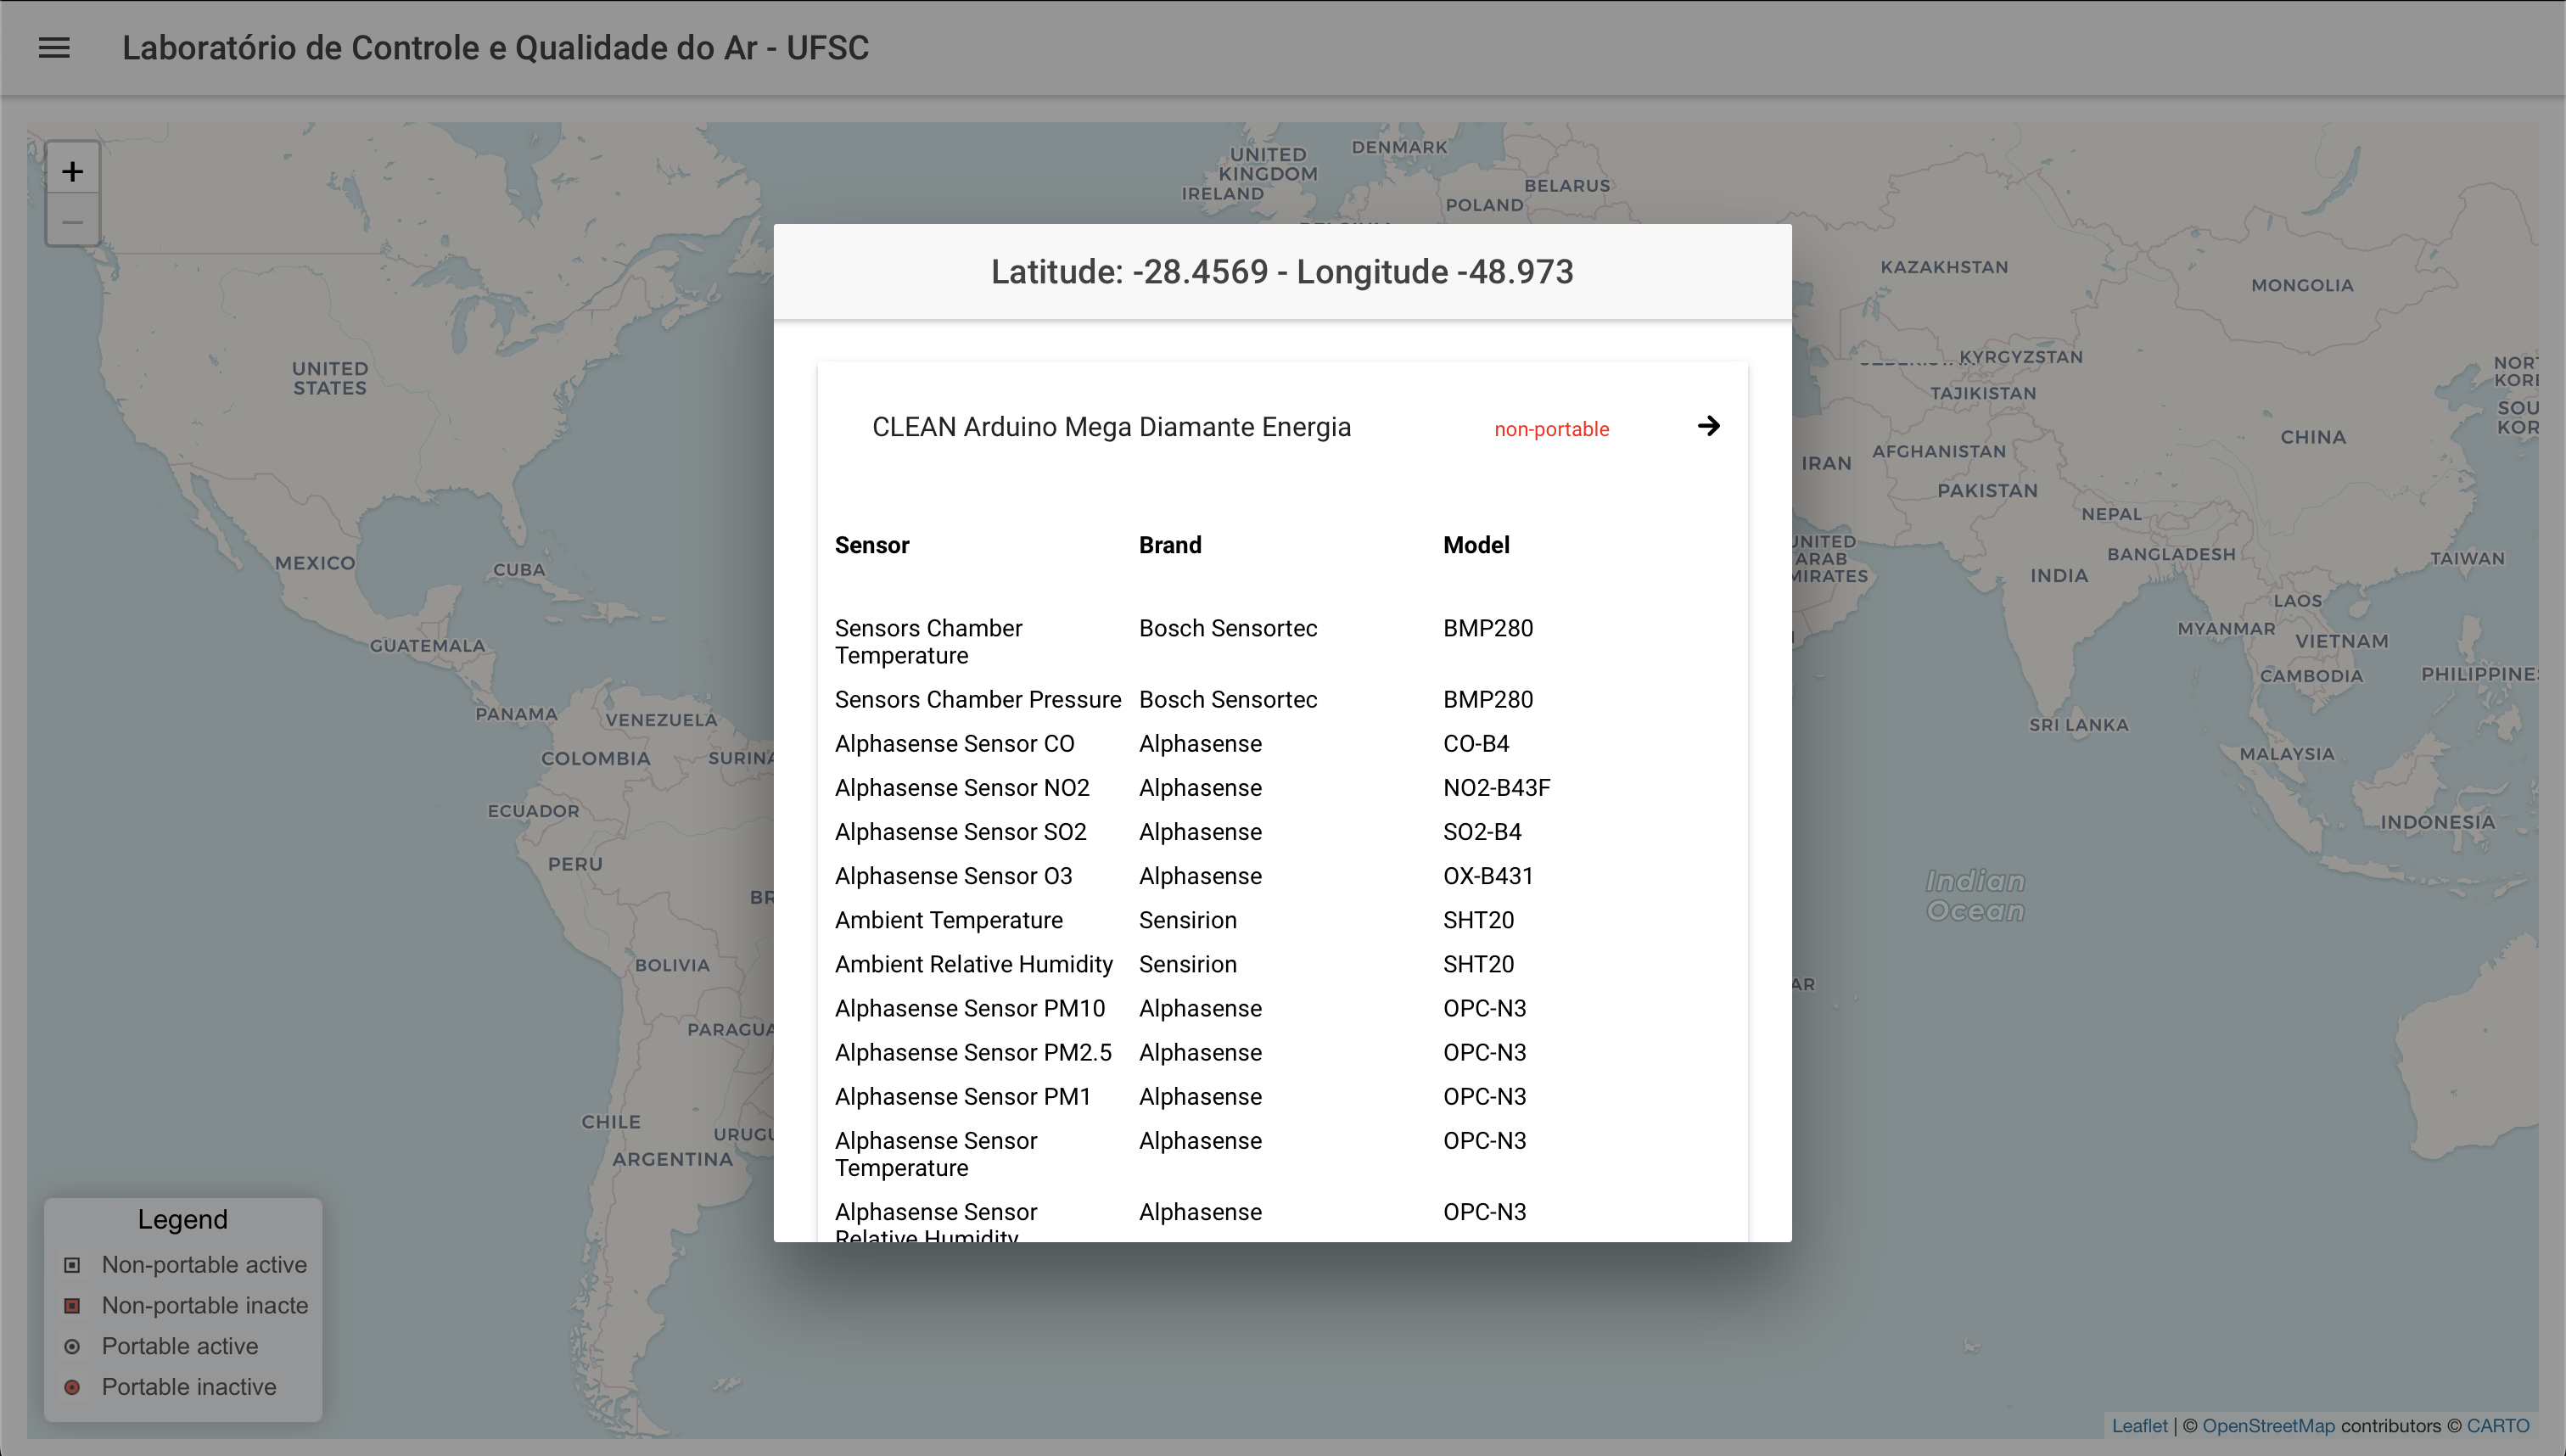
\includegraphics[width=\textwidth]{chapters/2-CLEAN/Figuras/Renovar Device Information.png}
        \caption{Painel de seleção de dispositivos}
        \label{fig:renovar-devices}
    \end{subfigure}
    \hfill
    \label{fig:renovar-map-and-devices}
    \fonte{Desenvolvido pelo autor (2023)}
\end{figure}

\begin{figure}[h]
    \centering
    \caption{Painéis da aplicação \textit{front-end} de Renovar}
    \begin{subfigure}{0.495\textwidth}
        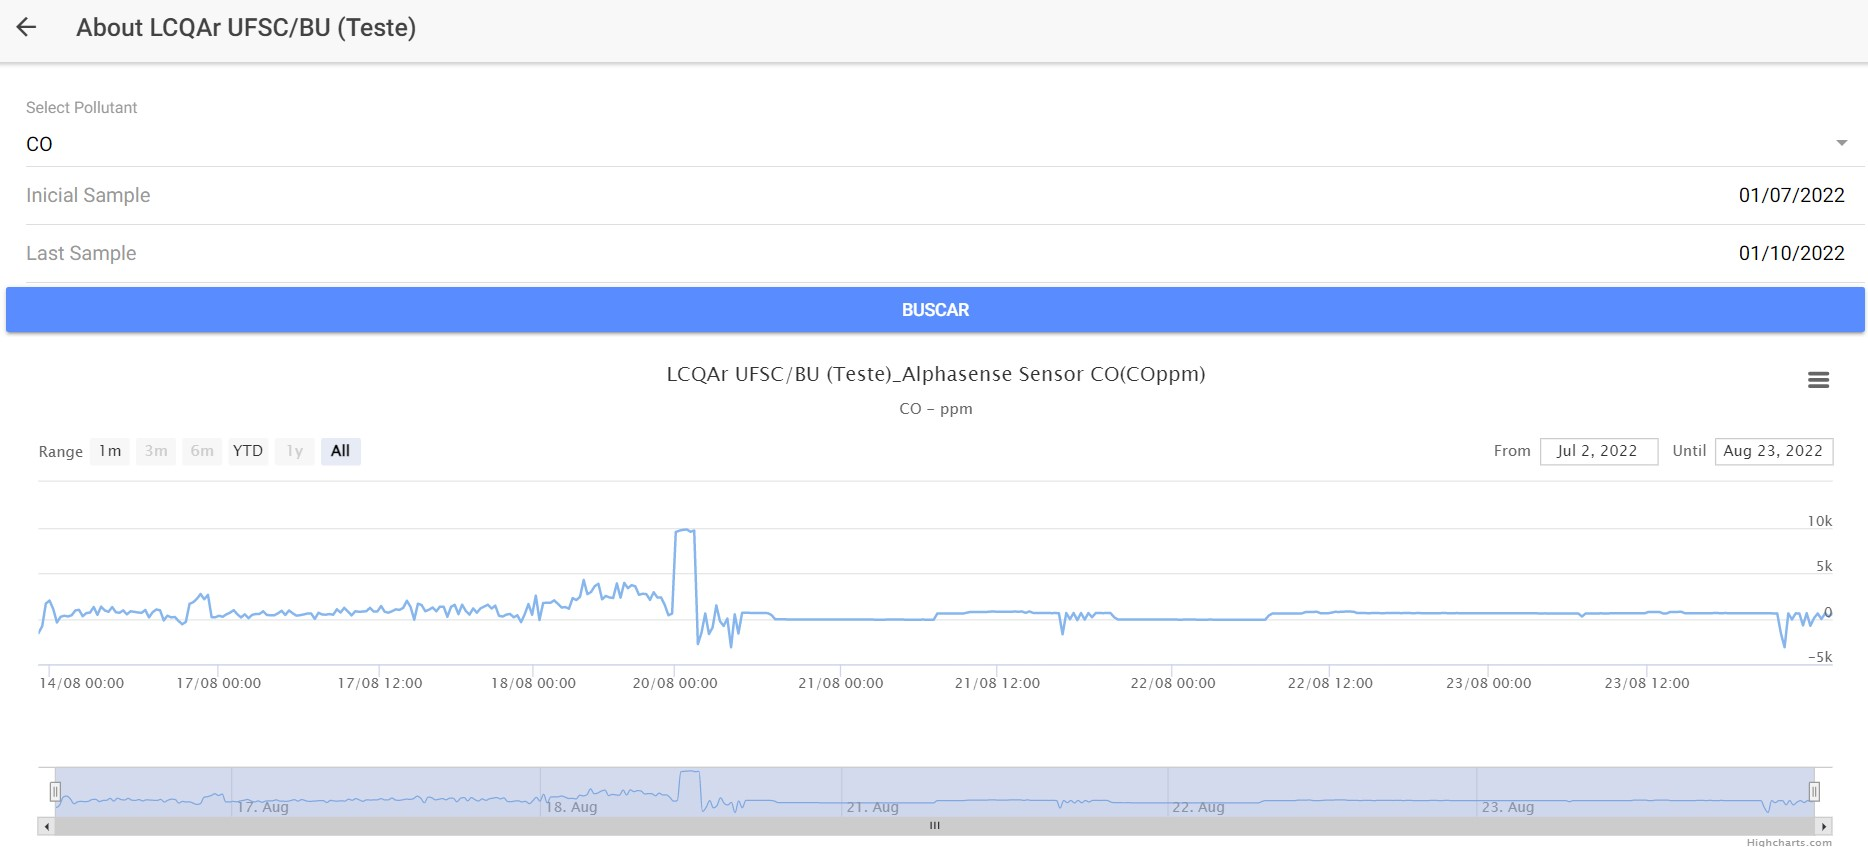
\includegraphics[width=\textwidth]{chapters/2-CLEAN/Figuras/ Renovar time series panel.jpg}
        \caption{Mapa de dispositivos}
        \label{fig:renovar-series-2}
    \end{subfigure}
    \hfill
    \begin{subfigure}{0.495\textwidth}
        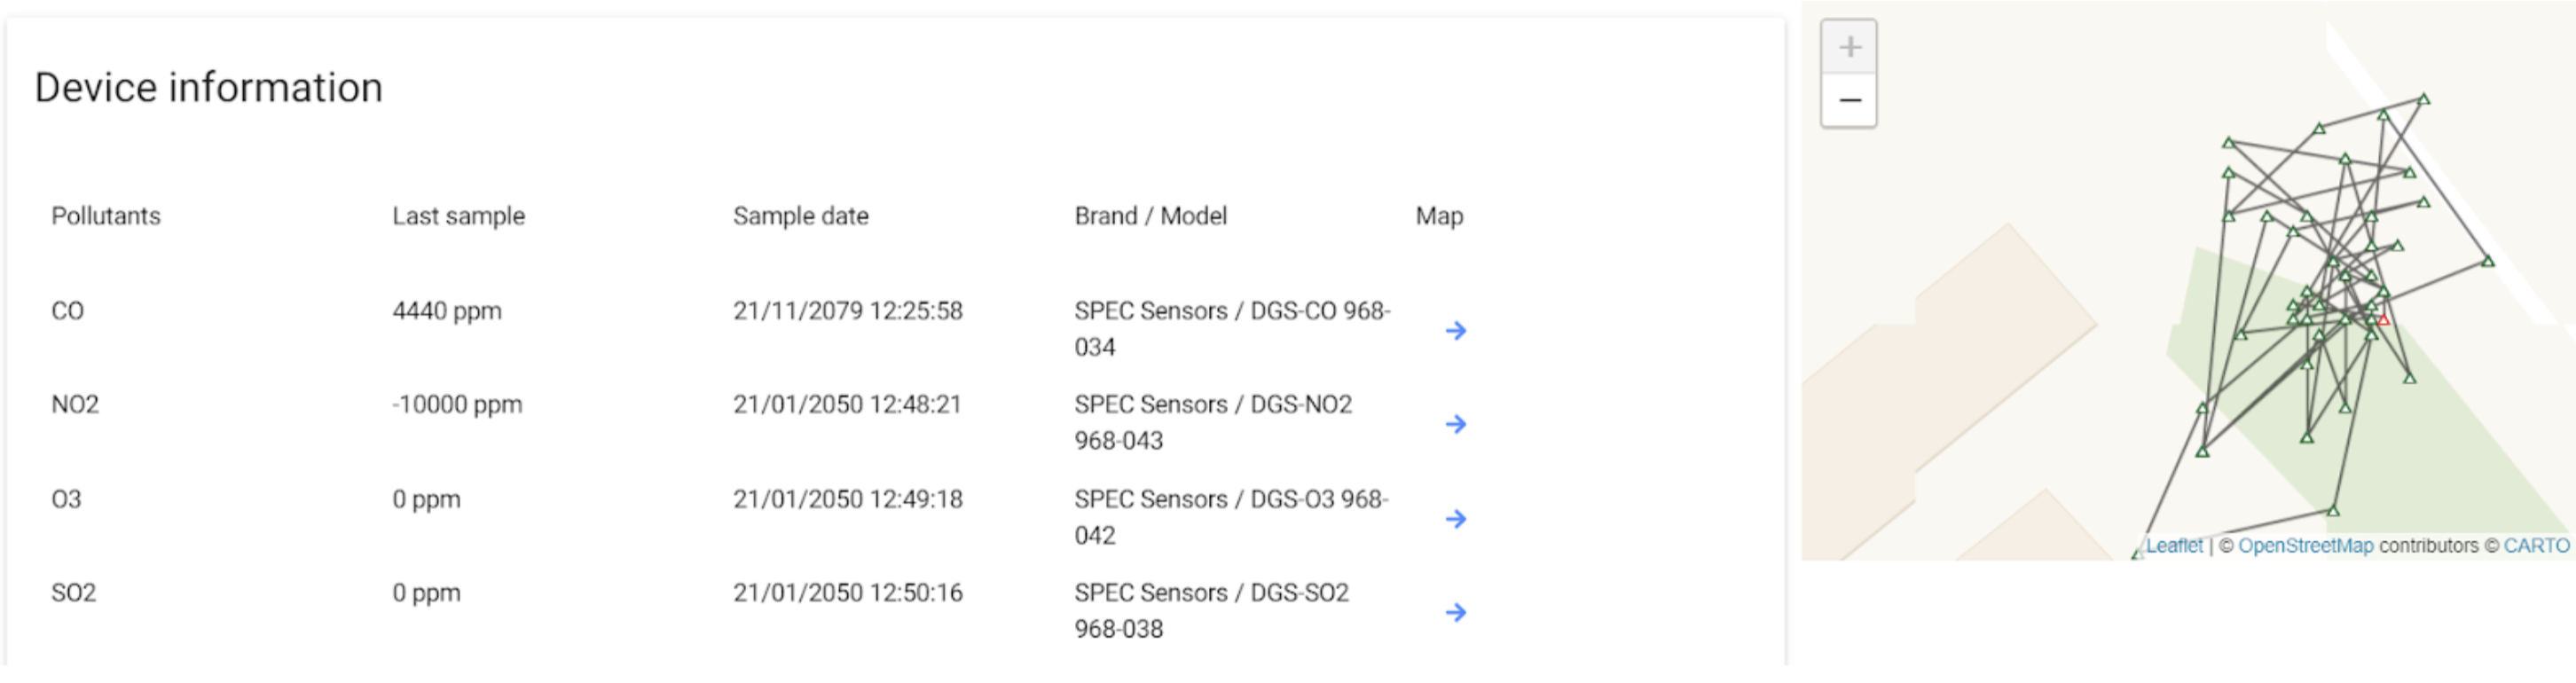
\includegraphics[width=\textwidth]{chapters/2-CLEAN/Figuras/Renovar portable map.png}
        \caption{Painel de seleção de dispositivos}
        \label{fig:renovar-portable-map}
    \end{subfigure}
    \hfill
    \label{fig:renovar-series-and-map}
    \fonte{Desenvolvido pelo autor (2023)}
\end{figure}

\begin{figure}[h]
    \centering
    \caption{Painel de análise de dados da aplicação \textit{back-end} Renovar}
    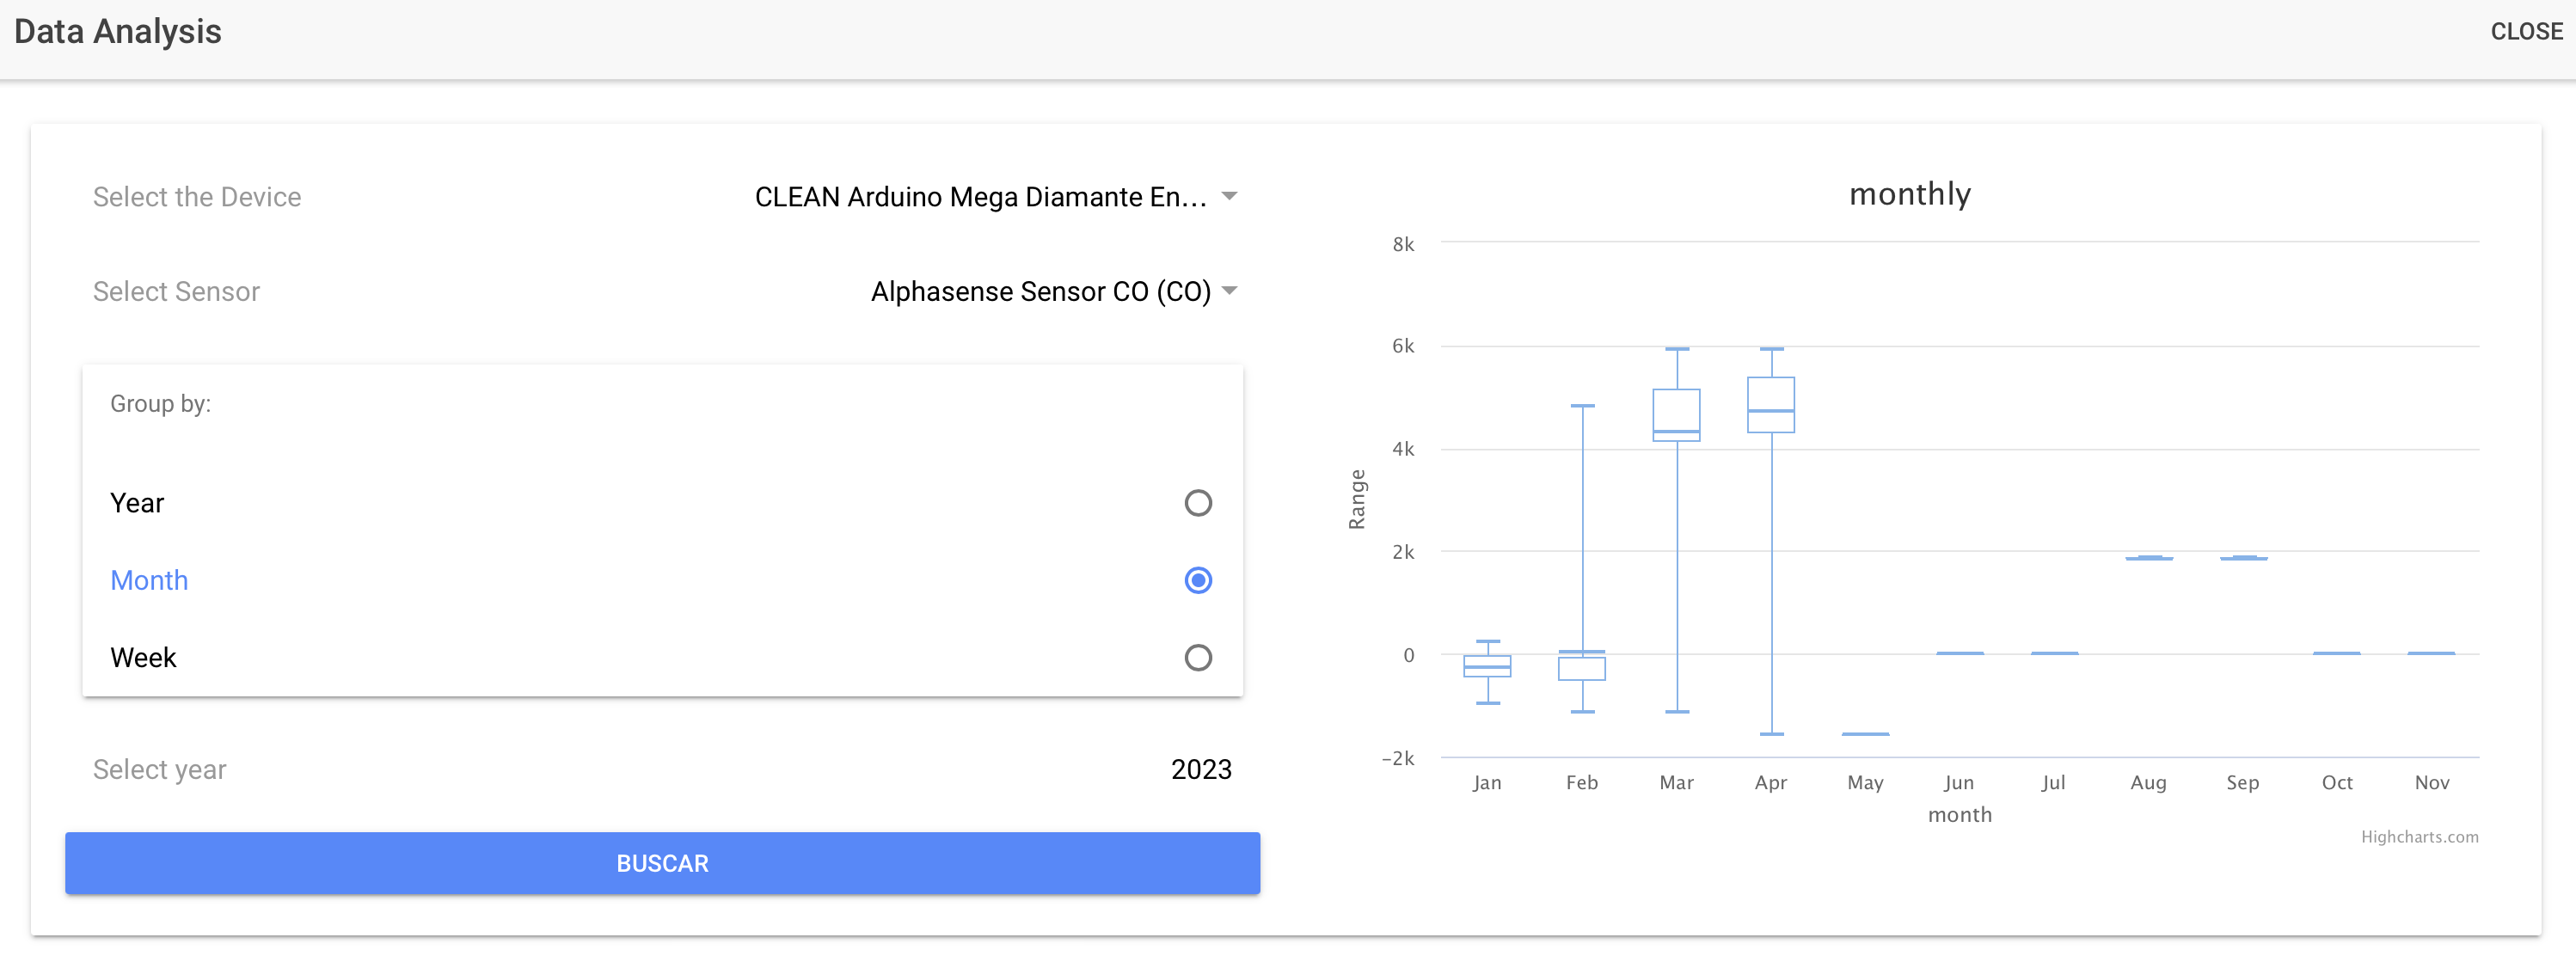
\includegraphics[width=0.80\linewidth]{chapters//2-CLEAN/Figuras/Renovar Data Analysis Panel.png}
    \label{fig:renovar-data-analysis}
    \fonte{Desenvolvido pelo autor (2023)}
\end{figure}

\section{Dispositivos de hardware desenvolvidos}

Dentro do contexto da iniciativa CLEAN foram desenvolvidos dispositivos para medição da qualidade do ar. Dois desses dispositivos foram protótipos para validação da ideia, concebidos para medições em locais fixos e medições móveis. Numa segunda etapa foram desenvolvidos dispositivos mais robustos com placas de circuito impresso e quadros elétricos para instalação em campo. A continuação serão descritos os equipamentos produzidos.

\subsection{Protótipos de monitores de qualidade do ar de baixo custo}

Foram concebidos dois protótipos de baixo custo para medição de poluentes atmosféricos \cite{Campo2020DEPLOYMENTRESULTS}, um para monitoramento fixo e outro para monitoramento móvel. O hardware de ambos os dispositivos, conforme mostrado na Figura \ref{fig:device-structure}, é composto por três blocos principais: 1) transporte de gás, 2) sensoriamento e 3) microcontrolador. O estágio de transporte de gás captura o ar ambiente nos sensores, que produzem um sinal analógico proporcional à concentração do gás. O microcontrolador, que é um Microchip ATMega2560 embarcado em uma plataforma Arduino Mega, captura as respostas dos sensores e as transforma em dados de concentração de gás. O hardware também obtém a hora e o local onde cada medição foi coletada. O microcontrolador armazena essas informações em um cartão micro SD e as transmite para um servidor web hospedado na Superintendência de Tecnologia da Informação e Comunicação da Universidade, rodando o aplicativo Renovar Web. Uma conexão Wi-Fi é estabelecida por um microcontrolador ESP8266 para transmissão de dados. Um relógio em tempo real e um módulo GPS fornecem informações de data, hora e geolocalização, respectivamente.

\begin{figure}
    \centering
    \caption{Estrutura principal dos dispositivos. a) Medidor de gases fixo, e b) medidor móvel}
    \includegraphics[width=1\linewidth]{chapters//2-CLEAN//Figuras/Estrutura geral protótipos.png}
    \label{fig:device-structure}
    \fonte{Desenvolvido pelo autor (2023)}
\end{figure}

A versão fixa dos dispositivos de monitoramento (Figura \ref{fig:device-structure}a) utiliza seis sensores eletroquímicos do fabricante de sensores Alphasense e quatro sensores eletroquímicos do fabricante SPEC Sensors. Para alimentação de energia do dispositivo utiliza-se uma fonte de 12VCC. Este dispositivo não incorpora módulo \textit{GPS} para geolocalização. A versão móvel (Figura \ref{fig:device-structure}b), por outro lado, utiliza apenas quatro sensores eletroquímicos do fabricante SPEC Sensors. O dispositivo é alimentado por um banco de energia de 5VCC através de uma conexão USB. A Figura 3 ilustra ambos protótipos na versão fixa e móvel. Mais detalhes sobre os dispositivos podem ser encontrados no Apêndice \ref{apendix: hw-prototypes}.

\begin{figure}
    \centering
    \caption{Ilustrações das versões (a) fixa e (b) móvel dos dispositivos de monitoramento}
    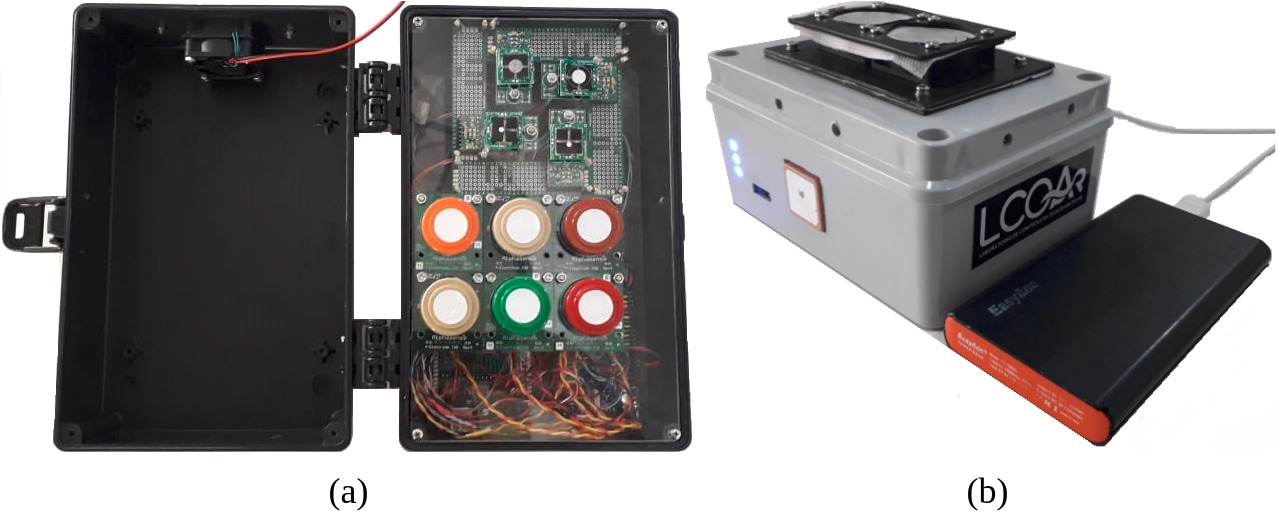
\includegraphics[width=1\linewidth]{chapters//2-CLEAN/Figuras/Monitoring Prototypes.jpg}
    \label{fig:monitoring-prototypes}
    \fonte{Desenvolvido pelo autor (2023)}
\end{figure}

\subsection{A placa CLEAN Arduino MEGA}

Com base nos resultados obtidos pelos protótipos e nas experiências alcançadas, foi desenvolvida uma versão mais compacta e atualizada para monitoramento fixo. Esta versão foi chamada de \textit{CLEAN Arduino Mega Board} por causa do microcontrolador Arduino Mega que ela usa como processador principal. A composição do hardware é muito semelhante à dos protótipos, mas os módulos foram montados em uma única \textit{PCB}. A Figura \ref{fig:clean-arduino-mega-board} ilustra o projeto da PCB e uma das placas fabricadas. A PCB foi criada no \textit{software} Eagle, e os arquivos do projeto estão disponíveis nos repositórios do LCQAr da UFSC.

\begin{figure}
    \centering
    \caption{A placa CLEAN Arduino Mega: (a) projeto PCB, (b) vista superior da placa, (c) vista inferior da placa.}
    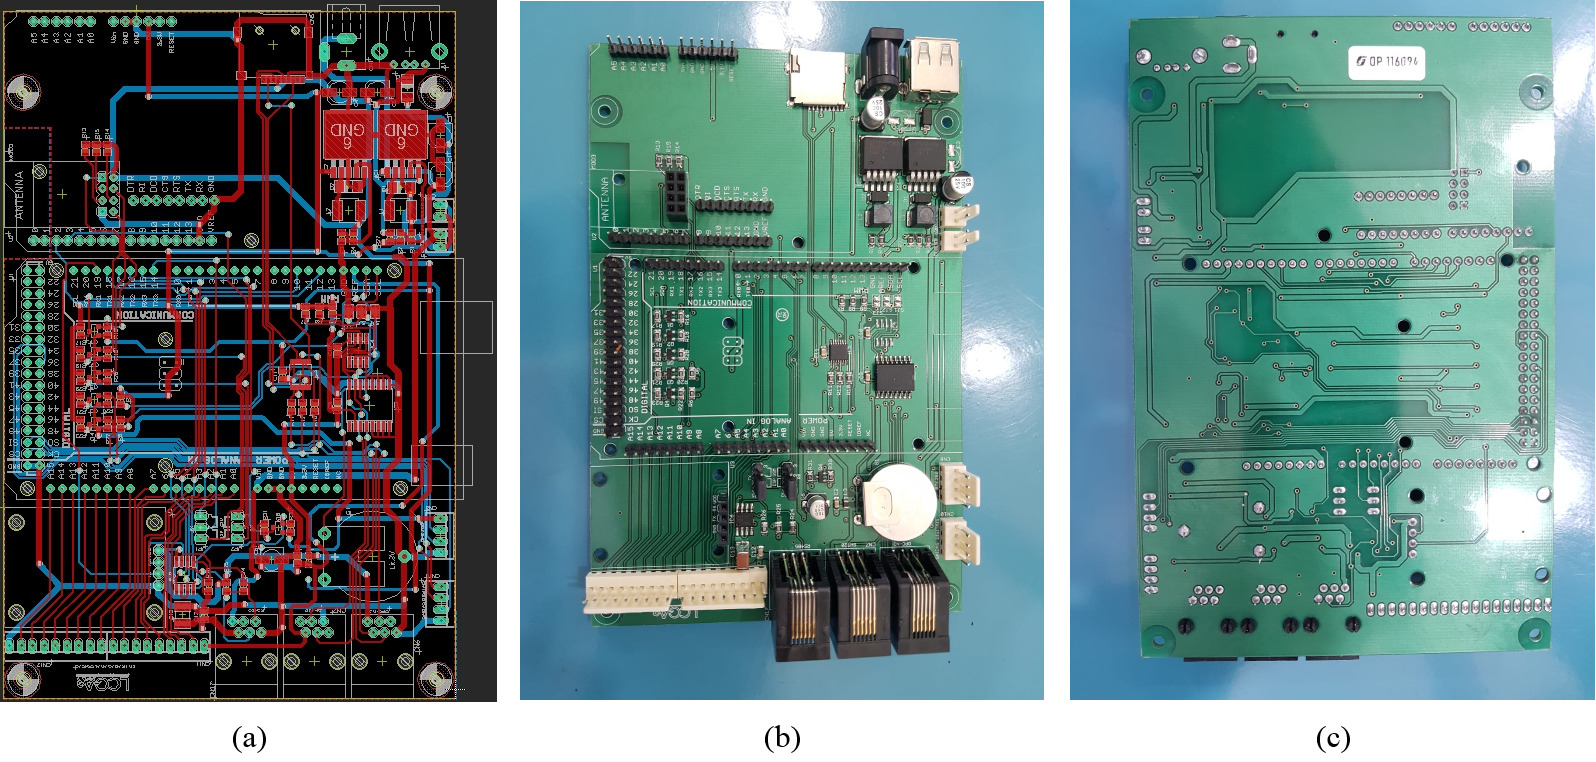
\includegraphics[width=1\linewidth]{chapters//2-CLEAN/Figuras/CLEAN Arduino Mega Board.jpg}
    \label{fig:clean-arduino-mega-board}
    \fonte{Desenvolvido pelo autor (2023)}
\end{figure}

A Tabela \ref{tab:componentes-clean} do apêndice \ref{apendix: clean-arduino-mega-board} mostra os principais componentes de hardware utilizados na placa, que requer uma tensão de alimentação de 12V, 2A através de um conector de alimentação P4. Possui entradas analógicas para 6 placas de sensores Alphasense da série ISB, barramento RS-485 para futuras expansões, três saídas digitais e conectores para alimentação de ventoinhas de 12V e 5V. A placa foi concebida para suportar conexões Wi-Fi e \textit{GPRS} à Internet. Essas conexões não podem ser utilizadas simultaneamente, o que dependerá de cada aplicação. O usuário pode configurar a placa para usar um ou outro e terá que adaptar o firmware do microcontrolador Arduino correspondentemente.


% ---

% ---
% 2 - Capítulo 2
% ---
\include{chapters/2-chapter}
% ---

% ---
% 3 - Capítulo 3
% ---
% ----------------------------------------------------------
\chapter{Seção}
% ----------------------------------------------------------

Este \textit{template} contém algumas seções criadas na tentativa de facilitar seu uso. No entanto, não há um limite máximo ou mínimo de seção a ser utilizado no trabalho. Cabe a cada autor definir a quantidade que melhor atenda à sua 
necessidade.  
% ---

% ---
% 4 - Conclusão
% ---
%\phantompart
% ----------------------------------------------------------
\chapter{Conclusão}
% ----------------------------------------------------------

Neste trabalho foi desenvolvida uma rede colaborativa para monitorização da qualidade do ar de baixo custo, a iniciativa CLEAN. Este iniciativa promove a colaboração para o desenvolvimento de plataformas de monitoramento de baixo custo, com custos mais baixos e com maior flexibilidade do que as atuais iniciativas de acesso aberto. A rede colaborativa pode incorporar um grupo mais amplo e diversificado de especialistas e entusiastas do monitoramento ambiental, aumentando a quantidade de dados disponíveis publicamente, diversificando as aplicações de monitoramento e melhorando a cobertura espaço-temporal da monitorização da qualidade do ar, especialmente nos países em desenvolvimento. CLEAN proporciona recursos de hardware e bibliotecas de firmware para diversas aplicações e usuários, assim como oferece uma aplicação backend e uma API REST, que facilita a integração de novos dispositivos à rede. Essa infraestrutura completa, aliada a uma aplicação frontend para visualização intuitiva dos dados, estabelece um ambiente para a integração de novos usuários e monitores, aumentando e diversificando o número de aplicações de monitoramento. O diferencial desta iniciativa com outras similares levantadas na revisão bibliográfica é que a estrutura modular das bibliotecas de firmware e a API para envio e leitura de dados para e do banco de dados contribuem na incorporação de novos colaboradores provém flexibilidade se para adaptar às especificações de cada aplicação e ao mesmo tempo uma estrutura sólida como base do desenvolvimento.

A iniciativa CLEAN promove a ciência cidadã, facilitando o processo de desenvolvimento dos dispositivos a um público mais vasto e disponibilizando dados sobre a qualidade do ar para análise e visualização. A rede de colaboradores pode se expandir para desenvolvedores, pesquisadores, amadores e estudantes que possam utilizar as ferramentas disponíveis no CLEAN para educação, prototipagem, uso pessoal e pesquisa. Uma cobertura mais ampla dos dados sobre a qualidade do ar disponibilizará uma quantidade considerável de dados, facilitando o acesso à informação ambiental para tornar as cidades e as povoações mais inclusivas, seguras, resilientes e sustentáveis. O acesso a informações representativas e fiáveis ajuda os investigadores e os decisores a encontrar soluções que promovam o florescimento de cidades mais inteligentes e saudáveis. Nos países em desenvolvimento, onde o acesso a tecnologias caras é mais limitado, iniciativas como o CLEAN são alternativas interessantes às redes de monitorização altamente dispendiosas que podem contribuir para o crescimento econômico sustentado e para um aumento da qualidade de vida dos cidadãos. Esta iniciativa tem potencial para expandir a comunidade de monitoramento do ar, especialmente no território brasileiro, e facilitar o acesso a informações sobre poluição atmosférica em regiões onde os dados regulatórios são escassos ou mesmo inexistentes.

Como parte da pesquisa também foram desenvolvidos e adicionados à rede, cinco dispositivos de medição de qualidade do ar, baseados no framework Arduino. Para validação das medições um dos equipamentos foi instalado junto a uma estação de referência por um período de 6 meses e suas leituras foram calibradas. Observou-se que as medições de \acrshort{no2} e \acrshort{so2} não puderam ser aproveitadas, indicando a necessidade de refinamento na aquisição de sinal para redução de ruído e estabilização do sinal de linha base. Os testes aprofundados com modelos de regressão multivariada, perceptron multicamadas, k vizinhos mais próximos e florestas aleatórias para calibrar as leituras de \acrshort{co}, \acrshort{o3} e \acrshort{mp10} revelam uma abordagem metódica e robusta em busca de precisão. A análise apurada indicou que as leituras de \acrshort{o3} produziram os melhores resultados com valores de r2 de 0.4. Observou-se também que quando combinadas com as leituras dos outros sensores aumentou a precisão das medições.

Como próximos passos, recomenda-se uma atenção especial para o aprimoramento do hardware de aquisição de sinal, com o objetivo de reduzir o ruído e estabilizar o sinal de linha base. Essas melhorias podem resultar em medições ainda mais precisas e confiáveis, consolidando a contribuição significativa deste trabalho na promoção do monitoramento de baixo custo da qualidade do ar em diversos contextos.
% ---

% ----------------------------------------------------------
% ELEMENTOS PÓS-TEXTUAIS
% ----------------------------------------------------------
\postextual
% ----------------------------------------------------------

% ----------------------------------------------------------
% Referências bibliográficas
% ----------------------------------------------------------
\begingroup
    \SingleSpacing\printbibliography[title=REFERÊNCIAS]
\endgroup

% ----------------------------------------------------------
% Glossário
% ----------------------------------------------------------
%
% Consulte o manual da classe abntex2 para orientações sobre o glossário.
%
% \glossary

% ----------------------------------------------------------
% Apêndices
% ----------------------------------------------------------

% ---
% Inicia os apêndices
% ---
\begin{apendicesenv}
%	\partapendices* 
	% ----------------------------------------------------------
\chapter{Descrição}
% ----------------------------------------------------------

Textos elaborados pelo autor, a fim de completar a sua argumentação. Deve ser precedido da palavra APÊNDICE, identificada por letras maiúsculas consecutivas, travessão e pelo respectivo título. Utilizam-se letras maiúsculas dobradas quando esgotadas as letras do alfabeto. 

\begin{quadro}[htb]
	\centering
	\caption{\label{qua:Quadro_2}Modelo A.}	
\begin{tabular}{|l|l|}
\hline
xxxx              & yyyyyyyyyyyyyyy    \\
\hline
xxxx              & yyyyyyyyyyyyyyy    \\
\hline
xxxx              & yyyyyyyyyyyyyyy    \\
\hline
xxxx              & yyyyyyyyyyyyyyy    \\
\hline
xxxx              & yyyyyyyyyyyyyyy    \\
\hline
xxxx              & yyyyyyyyyyyyyyy    \\
\hline
xxxx              & yyyyyyyyyyyyyyy    \\
\hline
rrrrrrrrrrrrrrrrr & eeeeeeeeeeeeeeeee  \\
\hline
xxxx              & yyyyyyyyyyyyyyy    \\
\hline
xxxx              & yyyyyyyyyyyyyyy    \\
\hline
rrrrrrrrrrrrrrrrr & eeeeeeeeeeeeeeeee  \\
\hline
xxxx              & yyyyyyyyyyyyyyy    \\
\hline
                  & ttttttttttttttttt  \\
\hline
rrrrrrrrrrrrrrrrr & eeeeeeeeeeeeeeeee  \\
\hline
ttttttttttttt     &                    \\
\hline
rrrrrrrrrrrrrrrrr & eeeeeeeeeeeeeeeee  \\
\hline
rrrrrrrrrrrrrrrrr & eeeeeeeeeeeeeeeee  \\
\hline
                  & gggggggggggggggggg \\
\hline
rrrrrrrrrrrrrrrrr & eeeeeeeeeeeeeeeee  \\
\hline
rrrrrrrrrrrrrrrrr & eeeeeeeeeeeeeeeee  \\
\hline
rrrrrrrrrrrrrrrrr & eeeeeeeeeeeeeeeee  \\
\hline
rrrrrrrrrrrrrrrrr & eeeeeeeeeeeeeeeee  \\
\hline
\end{tabular}
\fonte{Elaborada pelo autor (2016).}
\end{quadro}
    \input{aftertext/Operação sensores/operação_sensores_ec}
    \chapter{Protótipos de monitores da qualidade do ar desenvolvidos}\label{apendix: hw-prototypes}

Foram desenvolvidos dois protótipos para o monitoramento da qualidade do ar ilustrados na Figura \ref{fig:monitoring-prototypes} do Capítulo \ref{cap:clean-initiative}. Eles foram baseados na plataforma Arduino Mega 2560, que utiliza o microcontrolador ATMega2560 da Microchip. Um deles foi projetado para medição fixa em um local, e o outro para monitoramento de forma móvel. Este último, além de prover a informação temporal associada a cada leitura de concentração de poluente, inclui a localização onde a medição foi tomada. Os dispositivos foram projetados para a medição de poluentes regulados na Resolução CONAMA No. 491/2018, sendo eles: \acrshort{co}, \acrshort{no2}, \acrshort{so2} e \acrshort{o3}. Além desses gases, a versão fixa também inclui um sensor de sulfeto de hidrogênio ($H_2S$). 

A Figura \ref{fig:diagrama-sistemas} mostra diagramas com os módulos de \textit{hardware} que compõem os sistemas de medição fixo e móvel, sem incluir o processo de transporte dos gases. A versão fixa do sistema de monitoramento (Figura \ref{fig:estrutura-fixo}) utiliza seis sensores da empresa Alphasense sensíveis aos gases \acrshort{co}, \acrshort{no2}, \acrshort{so2}, \acrshort{o3} e $H_2S$. Além destes, também estão instalados quatro sensores da empresa SPEC, sensíveis aos mesmos poluentes com exeção do $H_2S$. A conexão entre a plataforma Arduino Mega e os sensores SPEC é realizada pela porta serial UART2 do microcontrolador através de um barramento RS-485. Já a leitura dos sensores da Alphasense é realizada pelas entradas analógicas AI0 – AI11 do microcontrolador.

\begin{figure}[h]
    \centering
    \caption{Diagrama de blocos dos sistemas fixo (a) e móvel (b)}
    \begin{subfigure}{0.495\textwidth}
        \centering
        \includegraphics[width=\textwidth]{aftertext/Protótipos desenvolvidos/Figuras/Estrutura versão fixa.png}
        \caption{}
        \label{fig:estrutura-fixo}
    \end{subfigure}
    \hfill
    \begin{subfigure}{0.495\textwidth}
        \centering
        \includegraphics[width=\textwidth]{aftertext/Protótipos desenvolvidos/Figuras/Estrutura versão móvel.png}
        \caption{}
        \label{fig:estrutura-mov}
    \end{subfigure}
    \label{fig:diagrama-sistemas}
    \fonte{Desenvolvido pelo autor (2023)}
\end{figure}

A versão móvel (Figura \ref{fig:estrutura-mov}) utiliza apenas sensores da SPEC para a medição de gases. Os modelos SPEC utilizados nesta versão são os mesmos que na versão fixa, e utilizam a mesma configuração para se comunicar de forma serial com o Arduino Mega. Um diferencial desta versão com relação à fixa, além de não utilizar sensores Alphasense, é a inclusão de um módulo GPS para georreferenciar as medições dos poluentes. O módulo utilizado é o GY-NEO6MV2 que se comunica com o microcontrolador através da UART1.

Além dos dispositivos mencionados acima, cada unidade de monitoramento inclui um módulo ESP8266 ESP-01 conectado à porta serial UART3 do Arduino, para comunicação Wi-Fi. Ambas unidades utilizam também um módulo de cartão micro SD para o armazenamento dos dados e um módulo de Relógio de Tempo Real (RTC) para manter a informação de data e hora. Outros periféricos como sensor de pressão, monitor LCD ou atuadores para controlar o transporte dos gases, podem ser adicionados através do barramento I2C em versões futuras.

Os módulos que compõem ambos sistemas de medição funcionam com tensões de alimentação tanto de 3.3 V como 5 V. Para fornecer esses níveis de voltagem foi utilizado um módulo-fonte que utiliza dois reguladores AMS1117. Um dos reguladores fornece uma saída 3.3 V e o outro 5 V. Ambos reguladores conseguem fornecer até 1 A de corrente de saída. O módulo-fonte possui dois canais de entrada de tensão. Um canal possui um conector Jack P4 para tensões entre 9 – 15 V, enquanto o outro possui um conector USB fêmea para fornecer uma tensão de 5 V.

O sistema fixo é alimentado com uma tensão de 12 V, aplicada no conector Jack P2 do módulo-fonte. Os 12 V de tensão podem ser provenientes de uma fonte conectada à rede elétrica, ou de um controlador solar conectado a um painel solar e uma bateria de 12 V. Já o sistema móvel pode ser alimentado por qualquer carregador de bateria portátil com saída em formato USB de 5 V e mínimo 2 A de corrente.

As seções seguintes descrevem cada um dos blocos que compõem os protótipos desenvolvidos.

\section{Transporte de gases}
\begin{table}
    \centering
    \caption{Especificações técnicas dos ventiladores utilizados no equipamento fixo e móvel}
    \begin{tabularx}{0.95\textwidth}[h]{
         >{\raggedright\arraybackslash}X
         >{\raggedright\arraybackslash}X 
         >{\raggedright\arraybackslash}X }
         \hline
        \textbf{Características} & \textbf{Versão fixa} & \textbf{Versão móvel} \\ [0.5ex] 
       \hline
        Descrição & Ventilador cooler 40mm 12VDC & Ventilador cooler 40mm 5VDC \\ 
        \hline
        Marca & GC & GDT \\ 
        \hline
        Tamanho & 40 x A: 40 x C: 10mm & L: 40 x A: 40 x C: 10mm \\
        \hline
        Corrente nominal & 80 ± 10\% mA & 140 ± 10\% mA \\
        \hline
        Tensão nominal & 12 V & Entre 5 e 7V \\
        \hline
        Ruído & 16 ± 10\% dBA & 16 ± 10\% dBA \\
        \hline
        Velocidade rotação & 5000 ± 10\% RPM & 7000 ± 20\% RPM \\
        \hline
        Fluxo de ar & 4.2 CFM & 6.12 CFM \\
        \hline
        Peso & 12 g & 14 g \\
        \hline
        Consumo potência & 1.2 W & 0.8 W \\
        \hline
        Vida útil & 35000 hr & 50000 hr \\
        \hline
    \end{tabularx}
    \label{tab:esp-ventiladores}
\end{table}

A etapa de transporte de gases é tida como a entrada do sistema. Sua função é capturar amostras do ar no ambiente e direcioná-las para o conjunto de sensores. Nos protótipos desenvolvidos, esta etapa é formada por dois ventiladores de corrente direta e uma câmara de gases. Os ventiladores conduzem o ar desde o ambiente de monitoramento até o interior da câmara. Esta última, por outro lado, consiste em um volume que retém o ar amostrado. No interior dela, os sensores são expostos às porções de ar coletadas para extrair informação de alguns poluentes que podem estar nelas contidos.

As configurações dos ventiladores variam de acordo com a versão do protótipo que os contêm. A versão fixa utiliza ventiladores com tensão nominal de 12 V, e a instalação mecânica deles foi realizada em série para conseguir maior pressão no fluxo do ar. Os ventiladores utilizados na versão móvel, por outro lado, têm uma tensão nominal de 5 V e foram colocados em paralelo. Suas características principais estão dispostas na Tabela \ref{tab:esp-ventiladores}.

\section{Sensoriamento}
A etapa de sensoriamento consiste em um arranjo de sensores de gases eletroquímicos e os circuitos de condicionamento analógico ou interfaces digitais correspondentes. Os sensores utilizados nos protótipos variam da versão fixa para a móvel, mas de forma geral foram instalados sensores do tipo \textit{screen-printed} fabricados pela SPEC Sensors LLC., e sensores da série B4 da Alphasense Ltd. Os dispositivos de transdução escolhidos são sensíveis aos poluentes regulados na Resolução CONAMA No. 491/2018: \acrshort{co}, \acrshort{no2}, \acrshort{so2}, \acrshort{o3}. Além desses gases, foi monitorado também o sulfeto de hidrogênio ($H_2S$) com um sensor de Alphasense. A modo de ilustração, a Figura \ref{fig:sensors} mostra os modelos SPEC DGS-CO 968-034 e Alphasense O3-B4, utilizados na medição de \acrshort{co} e \acrshort{o3}.

\begin{figure}[h]
    \centering
    \caption{Sensores dos fabricantes a) SPEC e b) Alphasense}
    \begin{subfigure}{0.495\textwidth}
        \centering
        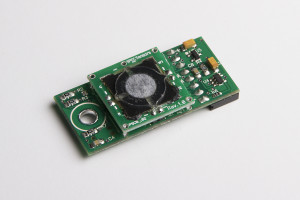
\includegraphics[width=\textwidth]{aftertext/Protótipos desenvolvidos/Figuras/SPEC IoT.jpg}
        \caption{}
        \label{fig:spec-iot}
    \end{subfigure}
    \hfill
    \begin{subfigure}{0.495\textwidth}
        \centering
        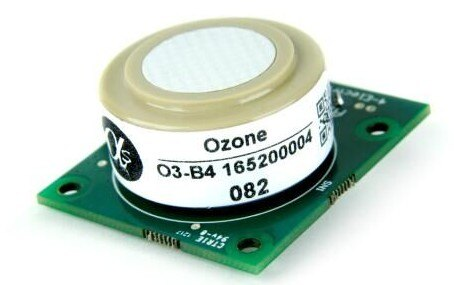
\includegraphics[width=\textwidth]{aftertext/Protótipos desenvolvidos/Figuras/Alphasense w ISB.jpg}
        \caption{}
        \label{fig:alpha-isb}
    \end{subfigure}
    \label{fig:sensors}
\end{figure}

A versão fixa dos instrumentos desenvolvidos contém arranjos de sensores das empresas SPEC e Alphasense. Já o equipamento móvel dispõe apenas de um arranjo de sensores da SPEC Sensors. A seguir são descritas características dos sensores de cada fabricante.

\subsection{Sensores SPEC}
Os sensores da SPEC possuem a configuração característica de três eletrodos (de trabalho, contador e de referência). A sigla SPEC provêm do inglês Screen-Printed Electro-Chemical, que é a tecnologia de manufatura utilizada por esse fabricante para produzir seus sensores. Essa tecnologia possibilita fabricar sensores de gases eletroquímicos de alta performance em um encapsulamento fino e de um custo menor que os encapsulamentos mais volumosos, utilizados tradicionalmente para fabricar sensores eletroquímicos \cite{SPECSensors2016SPECConsiderations}. A Figura \ref{fig:spec-iot} mostra o sensor SPEC DGS-CO 968-034, utilizado na medição de monóxido de carbono, em sua placa de condicionamento. A Tabela \ref{tab:esp-SPEC} resume as principais características dos sensores que foram utilizados dessa empresa. 

\begin{table}[b]
    \centering
    \caption{Especificações técnicas dos sensores SPEC}
    \label{tab:esp-SPEC}
    \begin{tabularx}{0.98\textwidth}[h]{
         >{\raggedright\arraybackslash}X
         >{\raggedleft\arraybackslash}X 
         >{\raggedleft\arraybackslash}X
         >{\raggedleft\arraybackslash}X 
         >{\raggedleft\arraybackslash}X }
         \hline
        \textit{Características} & $CO$ & $NO_2$ & $SO_2$ & $O_3$ \\
        \hline
        Modelo & DGS-CO 968-034 & DGS-NO2 968-043 & DGS-SO2 968-038 & DGS-O3 968-042 \\ 
        \hline
        Intervalo de medição & 0 - 1000 ppm & 0 - 5 ppm & 0 - 20 ppm & 0 - 5 ppm \\
        \hline
        Resolução & 100 ppb & 20 ppb & 50 ppb & 20 ppb \\
        \hline
        Tensão nominal & 3.3 V & 3.3 V & 3.3 V & 3.3 V \\
        \hline
        Consumo de potência & 12 mW & 14 mW & 12 mW & 14 mW \\
        \hline
        Tempo de resposta* & < 30 s & < 30 s & < 30 s & < 30 s \\
        \hline
        Temperatura de operação & -20 – 40 ºC & -20 – 40 ºC & -20 – 40 ºC & -20 – 40 ºC \\
        \hline
        Umidade relativa de operação & 15 – 95 \% & 15 – 95 \% & 15 – 95 \% & 15 – 95 \% \\
        \hline
    \end{tabularx}
\end{table}

\subsection{Sensores Alphasense}
Os sensores da série B4, da Alphasense, utilizam, além dos três eletrodos característicos do princípio de medição eletroquímico, um quarto eletrodo chamado de Eletrodo Auxiliar. Sua função é gerar uma corrente com um valor de intensidade muito próximo ao valor da corrente de fundo do zero (zero background current). Dessa forma é possível compensar a saída dos sensores do efeito desta corrente de zero ou de linha base. A Tabela \ref{tab:esp-ALPHA} resume as principais características dos sensores que foram utilizados desse fabricante.

\begin{table}
    \centering
    \caption{Especificações técnicas dos sensores Alphasense}
    \begin{tabularx}{0.98\textwidth}[h]{
        >{\raggedright\arraybackslash}X
        >{\raggedleft\arraybackslash}X
        >{\raggedleft\arraybackslash}X
        >{\raggedleft\arraybackslash}X
        >{\raggedleft\arraybackslash}X
        >{\raggedleft\arraybackslash}X }
        \hline
        \textit{Características} & $CO$ & $NO_2$ & $SO_2$ & $O_3$ & $H_2S$ \\
        \hline
        Modelo & CO-B4 & NO2-B43F & SO2-B4 & OX-B431 & H2S-B4 \\ 
        \hline
        Intervalo de medição (ppm) & 0 - 1000 & 0 - 20 & 0 - 100 & 0 - 20 & 0 - 100 \\
        \hline
        Resolução (ppb) & 4 & 15 & 5 & 15 & 1 \\
        \hline
        Tempo de resposta (s)* & < 30 & < 80 & < 60 &  < 80 & < 60 \\
        \hline
        Temperatura de operação (ºC) & -30 – 50 & -30 – 40 & -30 – 50 & -30 – 40 & -30 – 50 \\
        \hline
        Umidade relativa de operação (\%) & 15 – 90 & 15 – 85 & 15 – 90 & 15 – 85 & 15 – 90 \\
        \hline
    \end{tabularx}
    \label{tab:esp-ALPHA}
\end{table}

\section{Condicionamento}
A configuração mais utilizada nos circuitos de condicionamento dos sensores eletroquímicos é o potenciostato. Este circuito controla o potencial aplicado ao eletrodo de trabalho e converte a corrente desse eletrodo em um valor de tensão.

A empresa Alphasense disponibiliza para os sensores da série B4 uma placa de condicionamento chamada de \textit{Individual Sensor Board} (ISB). Esta placa transforma o sinal de corrente de saída do sensor em um sinal de tensão proporcional ao valor de concentração do gás. A SPEC Sensors, por sua vez, disponibiliza uma placa com um microcontrolador dedicado, que condiciona a saída do transdutor e entrega o dado de concentração mediante uma interface digital serial.

\subsection{Interface de condicionamento dos sensores Alphasense: A Placa de Sensoriamento Individual (ISB)}
As placas ISB da Alphasense possuem circuitos de potenciostato compatíveis com a família de sensores B4, de quatro eletrodos. Nesses circuitos, tanto o eletrodo de trabalho quanto o auxiliar possuem etapas de amplificação equivalentes. As tensões de saída destes dois eletrodos são disponibilizados em um conector Molex de 6 vías junto com os canais para a alimentação da placa. A tensão de alimentação das placas ISB pode ser entre 3.5 e 6.4 VDC; nos protótipos desenvolvidos foi utilizada uma tensão de 5 VDC.

O diagrama ilustrado na Figura \ref{fig:interface-alpha} apresenta as conexões realizadas entre a plataforma Arduino e os sensores da Alphasense através das placas ISB. Percebe-se que cada conjunto composto por um sensor e seu respectivo circuito de condicionamento, ocupa duas entradas analógicas do microcontrolador; uma entrada para o eletrodo auxiliar (AE) e outra para o eletrodo de trabalho (WE). No total foram utilizadas os canais analógicos A0 – A11.

\subsection{Interface de condicionamento dos sensores SPEC}
Assim como os sensores da Alphasense, os sensores da empresa SPEC também utilizam um circuito de condicionamento de potenciostato. Na mesma placa de condicionamento, a SPEC tem incorporado um microcontrolador dedicado e sensores de temperatura e umidade. O microcontrolador converte o valor de tensão de saída do potenciostato em um valor digital de concentração de gás, e realiza uma compensação, por software, dos efeitos da temperatura e a umidade na medição.

O kit de condicionamento SPEC funciona como uma camada de abstração no que diz respeito ao tratamento e condicionamento das informações, garantindo uma fácil integração com os sistemas de monitoramento. O dispositivo disponibiliza as informações de data e hora, o valor de concentração em ppm/ppb e as leituras de temperatura e umidade através de uma interface serial UART. De igual modo, podem ser realizadas operações como calibração, ajuste de zero e span, configuração dos sensores, e seleção de modo de operação de baixo consumo de energia, através de uma biblioteca com comandos pré definidos \cite{SPECSensors2017Digital968-045}.

\begin{figure}[t]
    \centering
    \caption{Interface entre os sensores e o microcontrolador Arduino. a) Alphasense, b) SPEC}
    \begin{subfigure}{0.39\textwidth}
        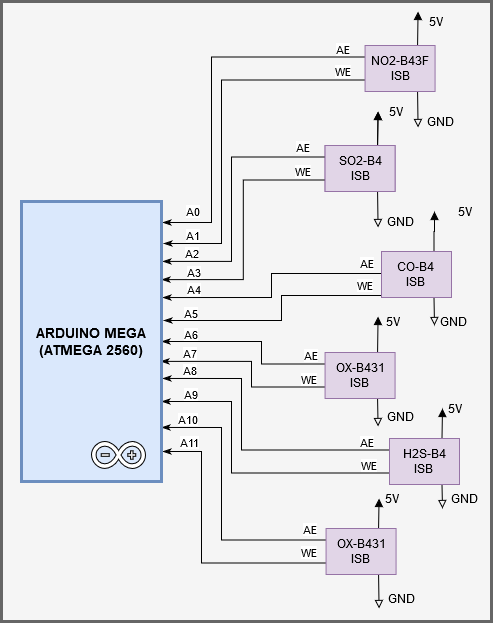
\includegraphics[width=\textwidth]{aftertext/Protótipos desenvolvidos/Figuras/Interface com sensores Alphasense.png}
        \caption{}
        \label{fig:interface-alpha}
    \end{subfigure}
    \hfill
    \begin{subfigure}{0.6\textwidth}
        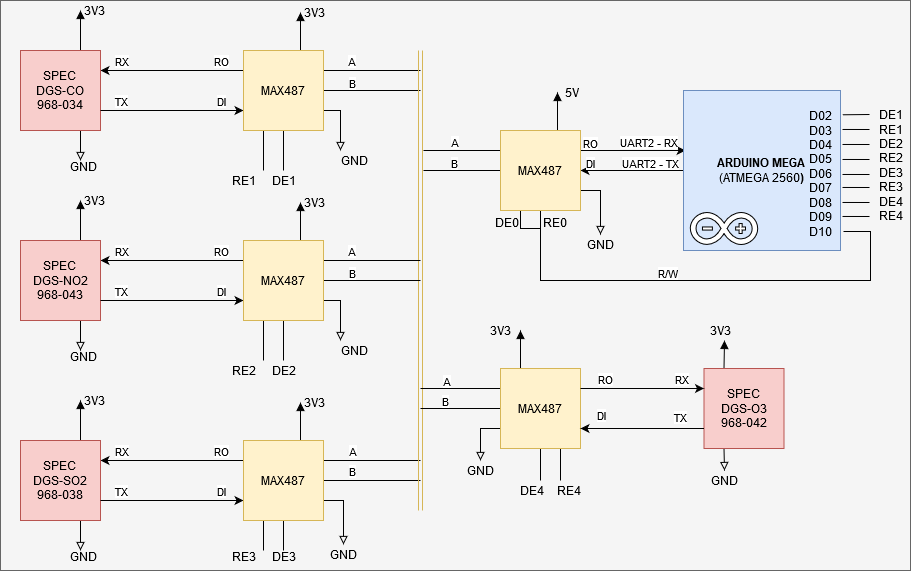
\includegraphics[width=\textwidth]{aftertext/Protótipos desenvolvidos/Figuras/Interface com sensores SPEC.png}
        \caption{}
        \label{fig:interface-spec}
    \end{subfigure}
    \hfill
    \label{fig:circuitos-interface}
    \fonte{Desenvolvido pelo autor (2023)}
\end{figure}

A Figura \ref{fig:interface-spec} apresenta um diagrama da conexão do arranjo de sensores da SPEC à plataforma Arduino Mega. Os sensores e o microcontrolador ATMega2560 são acoplados a um barramento RS-485 mediante o transceptor MAX487. Esse transceptor provê uma interface entre os meios de comunicação serial UART e RS-485. O barramento RS-485 consiste basicamente em dois fios A e B que fornecem o meio físico para a transmissão de níveis de tensão que representam os dados seriais enviados pelos diferentes dispositivos. O nível do sinal transmitido através do barramento é determinado pela tensão diferencial entre os conectores A e B, independentemente da voltagem de alimentação dos dispositivos conectados. Como mostra a figura, os transceptores dos sensores são alimentados com uma tensão de 3.3 VDC, enquanto o transceptor do Arduino é alimentado pelo mesmo sinal de 5 VDC que o microcontrolador.

É possível conectar múltiplos dispositivos a um mesmo barramento RS-485 (máximo até 128), sendo necessária a ação de um controlador que determine quem acessa o meio físico a cada instante, para evitar colisões. O microcontrolador ATMega2560 realiza essa função através das saídas digitais D02 – D10. Esses sinais digitais controlam o estado das entradas $RE_i$ e $DE_i$ de cada MAX487, a fim de habilitar/desabilitar cada transceptor para operações de escrita/leitura.

\section{Microcontrolador}
A etapa de processamento engloba todas as funcionalidades de controle, temporização, geolocalização, aquisição dos dados dos sensores, comunicação e armazenamento dos dados. Todas essas funções são gerenciadas pelo microcontrolador ATMega2560 da Microchip, embarcado na plataforma Arduino Mega 2560. Mais detalhes sobre o firmware desenvolvido para o controle da etapa de processamento são abordados no Apêndice \ref{appendix: firmware}. A continuação descrevem-se cada um dos módulos que compõem esta etapa.

\subsection{Armazenamento dos dados}
Para o armazenamento dos dados foi utilizado um módulo para fazer leitura e escrita diretamente em um cartão micro SD. A comunicação é feita por meio de uma interface SPI, conforme se mostra na Figura \ref{fig:interface-SD}. O nível de sinal é de 3.3V, mas o módulo possui divisores de tensão nos seus pinos que possibilitam uma ligação direta com placas que trabalham com 5 V, como o Arduino. O módulo é alimentado com uma tensão de 5 V, e suporta cartões Micro SD e Micro SDHC de alta velocidade.

\begin{figure}[h]
    \centering
    \caption{Interface entre o módulo cartão micro SD e o microcontrolador}
    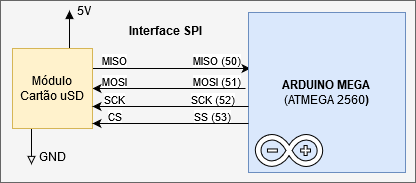
\includegraphics[width=0.7\textwidth]{aftertext/Protótipos desenvolvidos/Figuras/Interface com micro SD.png}
    \label{fig:interface-SD}
    \fonte{Desenvolvido pelo autor (2023)}
\end{figure}

\subsection{Controle de data e hora e geolocalização}
Para manter o controle da data e hora do sistema fixo, e assim acrescentar informação temporal às leituras de gases, foi utilizado o módulo de Relógio de Tempo Real (RTC) DS1307. O DS1307 é um relógio/calendário de baixo consumo de potência que utiliza um barramento $I^2C$ bidirecional para a transferência de dados desde (e para) o microcontrolador. O relógio/calendário provê informação de segundos, minutos, horas, dia, mês e ano, incluindo ajuste automático de ano bissexto e de meses com menos de 31 dias. O DS1307 é alimentado por uma tensão de 5 V, e também possui um circuito que detecta falhas de energia e automaticamente aciona a alimentação através de uma bateria. Quando isso sucede, o relógio/calendário mantém a contagem do tempo em um modo de baixo consumo (consumo de corrente menor que 500 nA), estendendo o tempo de vida útil da bateria. A Figura \ref{fig:interface-rtc} mostra como é realizada sua conexão ao microcontrolador no sistema desenvolvido.

\begin{figure}[h]
    \centering
    \caption{Interface entre o microcontrolador e os módulos a) RTC e b) GPS}
    \begin{subfigure}{0.49\textwidth}
        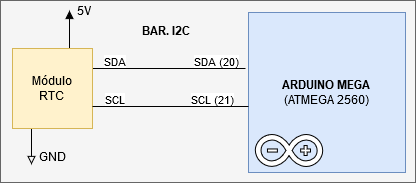
\includegraphics[width=\textwidth]{aftertext/Protótipos desenvolvidos/Figuras/Interface com RTC.png}
        \caption{}
        \label{fig:interface-rtc}
    \end{subfigure}
    \hfill
    \begin{subfigure}{0.49\textwidth}
        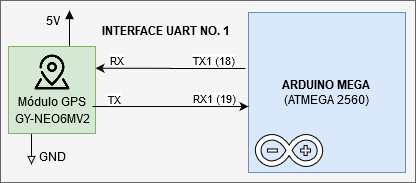
\includegraphics[width=\textwidth]{aftertext/Protótipos desenvolvidos/Figuras/Interface com GPS.png}
        \caption{}
        \label{fig:interface-gps}
    \end{subfigure}
    \hfill
    \label{fig:interface-RTC_GPS}
    \fonte{Desenvolvido pelo autor (2023)}
\end{figure}

Na versão móvel, ambos os controles da data e hora e geolocalização são realizados por um mesmo dispositivo GPS, o módulo NEO6MV2. O NEO6M é um receptor GPS de baixo consumo de potência e pequenas dimensões que o tornam uma opção interessante para dispositivos móveis. O módulo possui uma antena integrada, com precisão de aproximadamente 5 metros, e tecnologia para supressão de congestionamentos na comunicação e interferências. A conexão entre o módulo e a plataforma Arduino é realizada através de um barramento serial UART a uma taxa de transferência padrão de 9600 bauds (Figura \ref{fig:interface-gps}). Ele pode ser alimentado com uma tensão de 3.3 ou 5 V e seu consumo de corrente em pleno funcionamento chega a 45 mA. Seus pinos de entrada são compatíveis com níveis de tensão TTL e suportam tensões tanto de 5 como de 3.3 V, independentemente da tensão de alimentação.

\subsection{Comunicação Wi-Fi}
Para a comunicação Wi-Fi é utilizado o módulo ESP-01. Esse módulo incorpora o sistema integrado em um único chip (SoC, System on Chip) ESP8266EX, da empresa Espressif, e uma antena embarcada com ganho de potência de 3dBi, garantindo um alcance de até 90 metros em espaços abertos. O SoC ESP8266EX integra um processador de 32 bits, o Tensilica L106, que implementa os protocolos TCP/IP e o 802.11 b/g/n WLAN MAC. Ele possui como vantagens um baixo consumo de energia atrelado a uma velocidade de clock de 80 MHz. Sua memória RAM, disponível em aplicações em que o sistema está configurado como estação é de aproximadamente 36 kB. O módulo ESP-01 disponibiliza, para armazenar o programa de usuário, uma memória FLASH de 1MB externa que pode ser acessada por um barramento SPI. O módulo disponibiliza quatro portas digitais que são utilizadas principalmente para programar a FLASH de usuário e uma porta serial UART.

\begin{figure}[h]
    \centering
    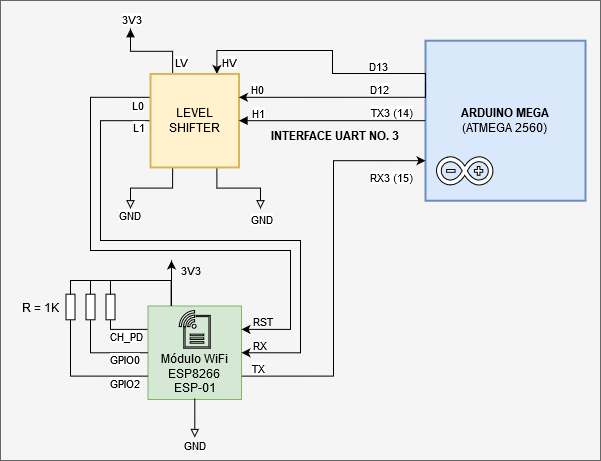
\includegraphics[width=0.6\textwidth]{aftertext/Protótipos desenvolvidos/Figuras/Interface com ESP8266.png}
    \caption{Interface entre o microcontrolador e o módulo de comunicação Wi-Fi}
    \label{fig:interface-esp}
    \fonte{Desenvolvido pelo autor}
\end{figure}

A Figura \ref{fig:interface-esp} apresenta as conexões realizadas entre o ESP-01 e a plataforma Arduino. O módulo opera com uma tensão de 3.3 V, por esse motivo é utilizado um circuito intermediário, um elevador de nível (level shifter) para converter os níveis de tensão de 5 V para 3.3 V, e vice-versa. O pino CH\_PD corresponde ao chip enable do ESP-01 e deve ser conectado a um resistor de \textit{pull-up} de 1 kΩ, assim como as entradas GPIO0 e GPIO2. Essas entradas são utilizadas para configurar o ESP8266 em modo gravação (para gravar o programa de usuário) ou modo estação. A figura mostra a configuração do modo estação, com ambas entradas conectadas à 3.3 V por meio de resistores de \textit{pull-up} de 1 kΩ. O pino de entrada RST tem como função reiniciar o módulo. Como esse pino é “ativo baixo”, cada vez que uma tensão de 0 V for aplicada nessa porta o módulo será reiniciado. No circuito desenvolvido, o Arduino pode reiniciar o ESP8266 através da saída digital D12. Já a saída D13 do microcontrolador Arduino é encarregada de manter uma tensão de referência de 5 V no elevador de nível para possibilitar a conversão dos níveis de tensão.

\section{Montagem do protótipo fixo}

A seguir descreve-se brevemente a montagem e interligação dos elementos de hardware que compõem o protótipo de medição fixa. A Figura \ref{fig:fixed-prototype-field-inst} mostra o protótipo de monitor fixo instalado em campo. O quadro externo é a caixa ambiental modelo Atlantic 352 00 da Cemar \& Legrand com nível de proteção IP66.

\begin{figure}[h]
    \centering
    \caption{Instalação em campo do protótipo fixo}
    \includegraphics[width=0.4\linewidth]{aftertext/Protótipos desenvolvidos/Figuras/Instalacão fixo.jpg}
    \label{fig:fixed-prototype-field-inst}
\end{figure}

As Figuras \ref{fig:fixed-prototype} e \ref{fig:fixed-prototype-int} mostram o módulo de sensoriamento, que é a parte fundamental de todo o sistema. Nele são contidos todos os elementos que compõem o sistema e que foram descritos anteriormente.

\begin{figure}[h]
    \centering
    \caption{Vista interior do protótipo fixo}
    \begin{subfigure}{0.495\textwidth}
        \centering
        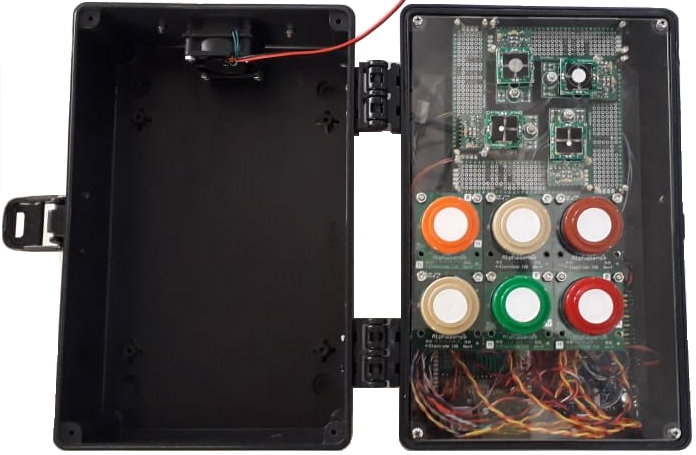
\includegraphics[width=\textwidth]{aftertext/Protótipos desenvolvidos/Figuras/clean-fixed-prototype.png}
        \caption{Vista superior}
        \label{fig:fixed-prototype}
    \end{subfigure}
    \hfill
    \begin{subfigure}{0.495\textwidth}
        \centering
        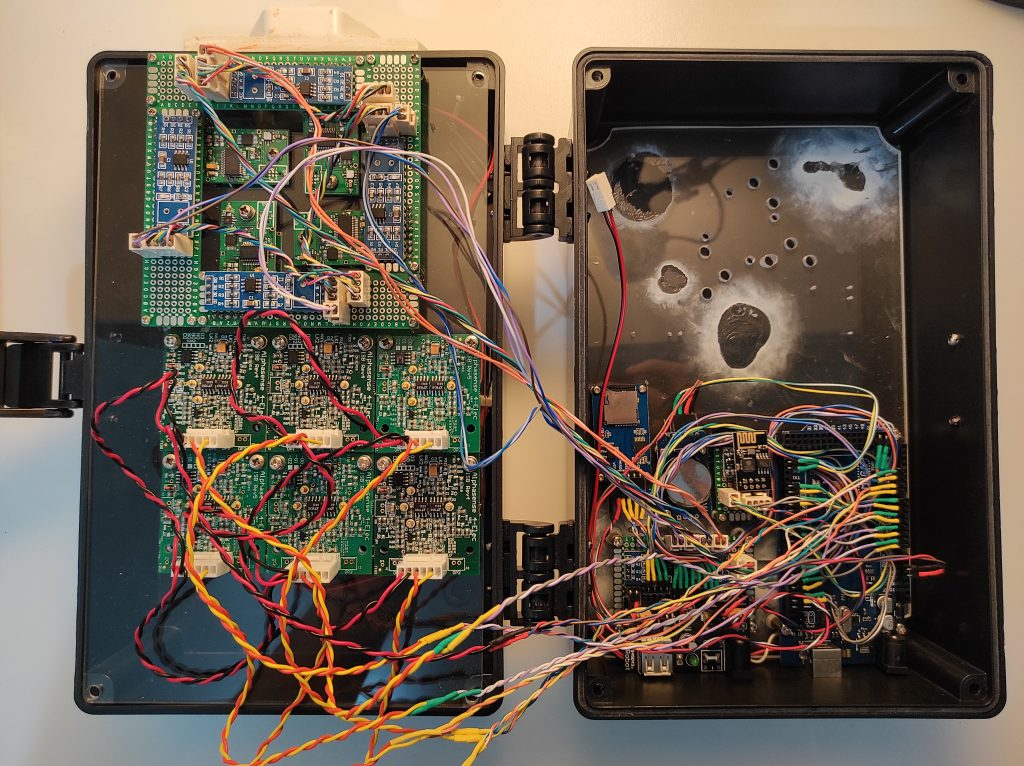
\includegraphics[width=\textwidth]{aftertext/Protótipos desenvolvidos/Figuras/clean-fixed-prototype-internal.jpg}
        \caption{Vista inferior}
        \label{fig:fixed-prototype-int}
    \end{subfigure}
    \label{fig:sensors}
\end{figure}

Um sistema de transporte de gases, composto por duas ventoinhas de 12VDC, coleta amostras do ar ambiente para dentro da câmara. A entrada é composta por uma flange de 50 mm de diâmetro (que serve para acoplar a câmara no restante do sistema de transporte de gases) e um filtro de tecido. As dimensões das ventoinhas são 40x40mm, e foram fixadas com quatro parafusos M2x30mm com porca e arruela. Dentro do volume da câmara, as superfícies dos sensores de gás interagem com os componentes gasosos e produzem um sinal de resposta proporcional à concentração do gás. A Tabela \ref{tab:list-of-sensors} resume os sensores e placas de condicionamento que foram utilizados nesssa versão do equipamento.

\begin{table}[h]
    \caption{Lista de sensores utilizados no protótipo fixo}
    \label{tab:list-of-sensors}
    \centering
    \begin{tabularx}{0.95\textwidth}[h]{
         >{\raggedright\hsize=.10\hsize\arraybackslash}X
         >{\raggedright\hsize=.40\hsize\arraybackslash}X 
         >{\raggedright\arraybackslash}X
         >{\raggedright\hsize=.30\hsize\arraybackslash}X }
        \hline
        \textbf{Qtd.} & \textbf{Ítem} & \textbf{Descrição} & \textbf{Fabricante}\\
        \hline
        1 & CO-B4 & Sensor de \acrshort{co} & Alphasense \\
        \hline
		1 & H2S-B4 & Sensor de \acrshort{h2s} & Alphasense \\
        \hline
		1 & SO2-B4 & Sensor de \acrshort{so2} & Alphasense \\
        \hline
        1 & NO-B4 & Sensor de \acrshort{no} & Alphasense \\
        \hline
        1 & NO2-B43F & Sensor de \acrshort{no2} & Alphasense \\
        \hline
        1 & OX-B431 & Sensor de \acrshort{o3} & Alphasense \\
        \hline
        1 & NH3-B1 & Sensor de \acrshort{nh3} & Alphasense \\
        \hline
        3 & CO/H2S/SO2 4-electrodes ISB & Placa de condicionamento para sensores da série B4 que medem \acrshort{co}, \acrshort{h2s} e \acrshort{so2} & Alphasense \\
        \hline
        1 & NO 4-electrodes ISB & Placa de condicionamento para sensores da série B4 que medem \acrshort{no} & Alphasense \\
        \hline
        1 & NO2/O3 4-electrodes ISB & Placa de condicionamento para sensores da série B4 que medem \acrshort{no2} e \acrshort{o3} & Alphasense \\
        \hline
        1 & NH3 4-electrodes ISB & Placa de condicionamento para sensores da série B4 que medem \acrshort{nh3} & Alphasense \\
        \hline
        1 & DGS-O3-968-042\_9-6-17 & Sensor de \acrshort{o3} para \acrshort{iot} & SPEC Sensors \\
        \hline
        1 & DGS-SO2-968-038 & Sensor de \acrshort{so2} para \acrshort{iot} & SPEC Sensors \\
        \hline
        1 & DGS-NO2-968-043-9-6-17 & Sensor de \acrshort{no2} para \acrshort{iot} & SPEC Sensors \\
        \hline
        1 & DGS-CO-968-034 & Sensor de \acrshort{co} para \acrshort{iot} & SPEC Sensors \\
        \hline
    \end{tabularx}
\end{table}

Uma placa de acrílico foi utilizada para fixar os sensores de maneira correta e isolar o \textit{hardware} do fluxo de ar. As conexões elétricas para levar os sinais de saída dos sensores até o Arduino foram feitas com fios de seção 0,2mm², soldando “\textit{headers}” nas pontas e isolando-as corretamente com duto termorretrátil. As Figuras \ref{fig:alphasense-power-supply} e \ref{fig:alphasense-connections} ilustram respectivamente diagramas de conexão da alimentação elétrica e dos eletrodos dos sensores ao Arduino.

\begin{figure}[h]
    \centering
    \caption{Diagrama de conexões do conjunto de sensores Alphasense}
    \begin{subfigure}{0.495\textwidth}
        \centering
        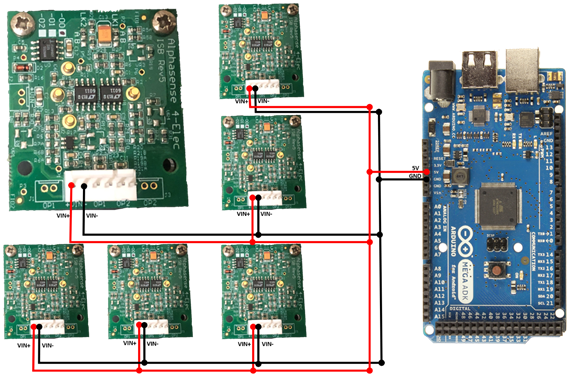
\includegraphics[width=\textwidth]{aftertext/Protótipos desenvolvidos/Figuras/Alimentação Alphasense.png}
        \caption{Alimentação elétrica}
        \label{fig:alphasense-power-supply}
    \end{subfigure}
    \hfill
    \begin{subfigure}{0.495\textwidth}
        \centering
        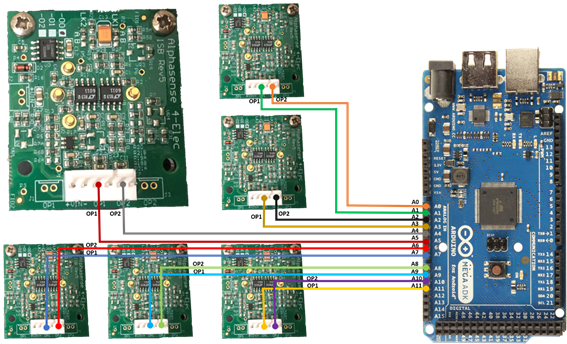
\includegraphics[width=\textwidth]{aftertext/Protótipos desenvolvidos/Figuras/Conexões Alphasense.png}
        \caption{Conexão dos eletrodos}
        \label{fig:alphasense-connections}
    \end{subfigure}
\end{figure}

A fixação dos sensores \textit{SPEC} na placa de acrílico mencionada anteriormente foi feita através de placas de prototipagem confeccionadas artesanalmente. Nas placas foram soldados “\textit{headers}” fêmeas encima dos quais os sensores foram montados. Nas placas também foram instalados os transceptores MAX487 que criam o barramento RS-485 para a conexão serial com o microcontrolador da placa Arduino. As placas são conectadas ao barramento através de fios e conectores do tipo MOLEX. As placas de prototipagem com os sensores foram fixadas diretamente à placa de acrílico com espaçadores M2.

Após a montagem do conjunto de sensores e prefixação dos componentes eletrônicos da câmara de medição, foi realizada a ligação elétrica de alimentação e comunicação de todos os componentes envolvidos no sistema. O diagrama de alimentação é mostrado na Figura \ref{fig:fixed-modules-power-supply}. Vale salientar que a alimentação da placa Arduino foi feita diretamente com 12V com fios soldados no conector P2 de entrada. Já a conexão do restante dos módulos com a placa Arduino é ilustrada na Figura \ref{fig:fixed-modules-connections}.

\begin{figure}[h]
    \centering
    \caption{Diagrama de conexões do conjunto de sensores Alphasense}
    \begin{subfigure}{0.495\textwidth}
        \centering
        \includegraphics[width=\textwidth]{aftertext/Protótipos desenvolvidos/Figuras/alimentação_fixo.png}
        \caption{Alimentação dos módulos do protótipo}
        \label{fig:fixed-modules-power-supply}
    \end{subfigure}
    \hfill
    \begin{subfigure}{0.495\textwidth}
        \centering
        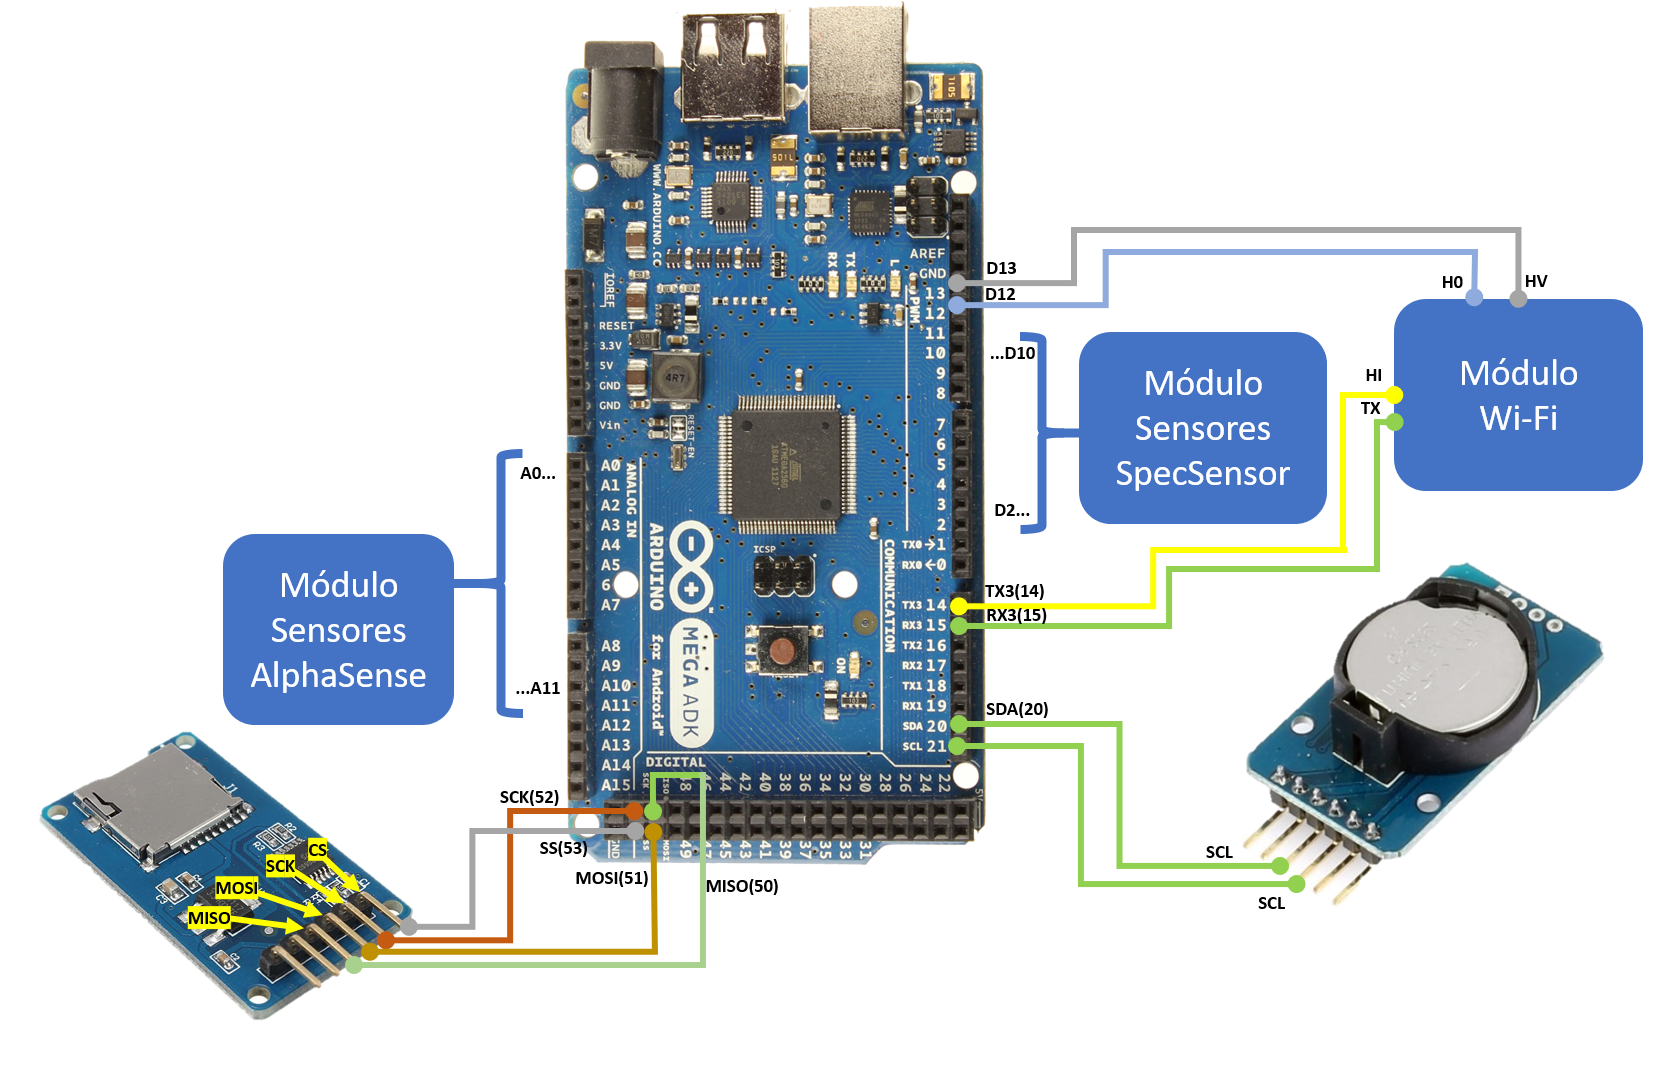
\includegraphics[width=\textwidth]{aftertext/Protótipos desenvolvidos/Figuras/comunicacao_fixo.png}
        \caption{Conexão dos módulos do protótipo}
        \label{fig:fixed-modules-connections}
    \end{subfigure}
\end{figure}

\section{Montagem do protótipo móvel}

O equipamento mede poluentes da legislação ambiental brasileira \cite{BRASIL.MINISTERIODOMEIOAMBIENTEMMA.ConselhoNacionaldoMeioAmbienteCONAMA2018ResolucaoAr.} que são: \acrshort{co}, \acrshort{no2}, \acrshort{so2}, \acrshort{o3} e \acrshort{h2s}. Para isso utiliza um conjunto de quatro sensores do fabricante SPEC Sensor que contemplam a medição desse poluentes. O controle da estapa de monitoramento, armazenamento e envio de dados é baseado na plataforma Arduino Mega 2560, que utiliza o microcontrolador ATMega2560 da Microchip. Para operar com sucesso, o sistema inclui: módulo Wi-Fi, módulo de cartão SD, módulo GPS e indicadores LED operacionais.
    % -------------------------------------------------------------------
\chapter{A placa \textit{CLEAN Arduino Mega}}\label{apendix: clean-arduino-mega-board}
% -------------------------------------------------------------------

A continuação são descritos os principais módulos que compõem a placa CLEAN Arduino Mega e os protótipos desenvolvidos. A Tabela \ref{tab:componentes-clean} mostra os principais componentes de hardware utilizados sem considerar os sensores.

\begin{table}
    \caption{Principais componentes utilizados nos dispositivos CLEAN}
    \label{tab:componentes-clean}
    \centering
    \begin{tabularx}{0.95\textwidth}[h]{
         >{\raggedright\arraybackslash}X
         >{\raggedright\arraybackslash}X 
         >{\raggedright\arraybackslash}X }
        \hline
        \textbf{Item} & \textbf{Descrição} & \textbf{Modelo e fabricante}\\ \hline
        Arduino Mega 2560 & Placa microcontroladora baseada no microcontrolador Microchip ATmega2560 & Arduino MEGA 2560 Rev3, de Arduino\\ \hline
		DS3231 RTC & Relógio em tempo real (RTC) I2C com oscilador de cristal compensado por temperatura integrado & DS3231, by Maxim Integrated\\ \hline
		Soquete micro SD & Soquete TF / micro SD tipo PUSH-PUSH & KLS1-TF-007, da KLS Electronic\\ \hline
        Buffer CI 74XX125 & Portas de buffer de barramento quádruplas com saídas de 3 estados para buffer de pinos de cartão micro SD & 74HC125, da Texas Instruments\\ \hline
        Cartão MicroSD & Cartão Micro SD Classe 10 de 16 GB & microSDHC SanDisk Ultra, da SanDisk\\ \hline
        Módulo GPS & Módulo GPS NEO-6M c/ antena & GY-GPS6MV2, por u-blox\\ \hline
        Módulo GPRS & Shield Arduino - GSM GPRS SIM900 com antena Quad Band & SIM900, da SIMCom\\ \hline
        Módulo Wi-Fi & Módulo serial Wi-Fi ESP-01 ESP8266 & ESP8266, da Expressif\\ \hline
        Sensor BMP280 & Sensor digital de temperatura e pressão BMP280 I2C & BMP280, da Bosch Sensortec\\ \hline
        Sensor SHT20 & Sensor de umidade e temperatura SHT20 I2C & SHT20, por Sensirion\\ \hline
    \end{tabularx}
\end{table}

\section{Módulo de sensoriamento}
\subsection{Sensores}

Nos sistemas desenvolvidos foram utilizados sensores do fabricante \textit{Alphasense} de princípio eletroquímico para medição de gases e contadores óticos de partículas para medição de material particulado.

\subsubsection{Sensores eletroquímicos Alphasense.}

\textit{Alphasense} fabrica sensores eletroquímicos amperométricos. Especificamente, os sensores da série B4 foram selecionados para os monitores desenvolvidos, já que são indicados pelo fabricante para a medição de baixas concentrações de gases. Estes sensores incorporam um quarto eletrodo, denominado eletrodo auxiliar, que compensa os efeitos da temperatura e da umidade relativa nas leituras dos sensores \cite{Baron2017AmperometricReview}. A Figura \ref{fig:alphasense-b4} ilustra um sensor Alphasense da série B4, suas dimensões e disposição dos eletrodos. Para mais informações sobre os efeitos das variáveis ambientais nas respostas dos sensores, confira a nota de aplicação AAN 110 da Alphasense. Para informações adicionais sobre os sensores da série B4 da Alphasense, como especificações elétricas, dimensões e pinagem, consulte as fichas técnicas dos modelos de sensores listados na Tabela 1.

\begin{figure}
    \centering
    \caption{Sensor de Monôxido de Nitrogênio Alphasense da série B4}
    \begin{center}
        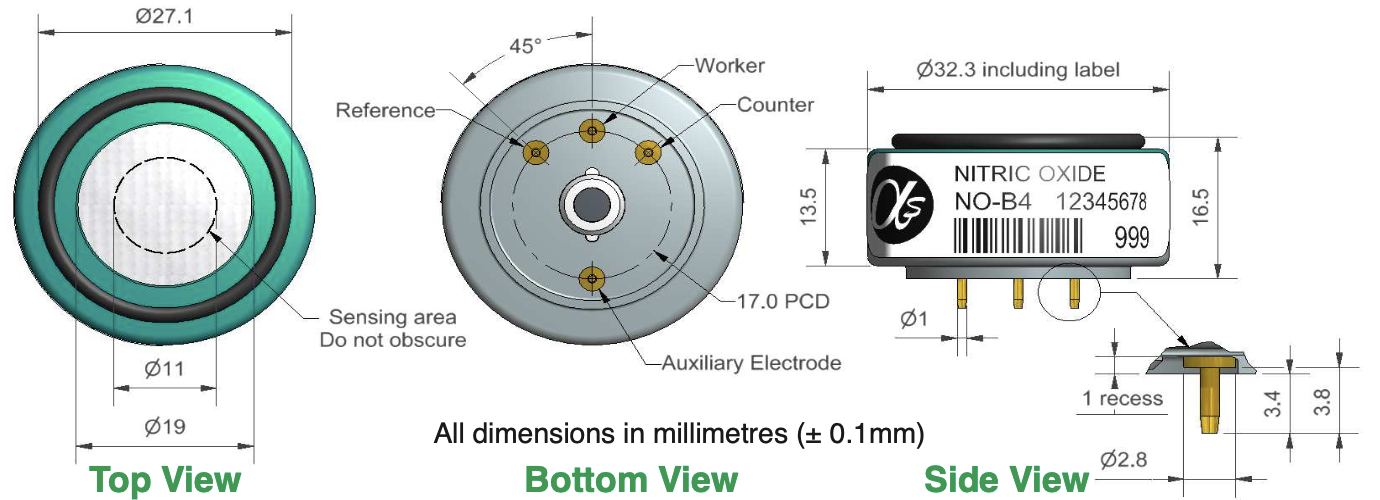
\includegraphics[width=0.75\textwidth]{aftertext/Principais componentes de hardware/Figuras/Sensores serie B4.png}
    \label{fig:alphasense-b4}
	\fonte{\cite{Alphasense2019NO-B4Sensor}.}
    \end{center}
\end{figure}

Sensores eletroquímicos amperométricos produzem uma corrente de saída que é proporcional à concentração do gás. Para ler este sinal elétrico com um sistema de aquisição de dados, a corrente de saída deve ser transformada em um sinal de tensão. Para isso, o circuito mais utilizado é o potenciostato. \textit{Alphasense} e \textit{SPEC} fornecem placas de circuito potenciostato para acoplar facilmente seus sensores a um sistema de monitoramento.

\subsubsection{Interface de condicionamento de sensores SPEC}

Os sensores digitais para IoT fornecidos pela SPEC são compostos por um transdutor eletroquímico montado em uma placa com um circuito potenciostato, que converte a saída do sensor (corrente elétrica) a tensão. Os sensores incorporam também um microcontrolador e um sensor de temperatura e umidade relativa. O microcontrolador adquire o sinal de tensão do potenciostato como valores de concentração de gás e realiza uma compensação em software para reduzir os efeitos da temperatura e a umidade relativa nas leituras do sensor. Os valores de concentração, temperatura e umidade relativa são transmitidos através de uma interface UART seguindo um protocolo serial definido pelo fabricante. Esta placa de condicionamento atua como uma camada de abstração para condicionamento de sinal que permite a fácil integração dos sensores a qualquer sistema de monitoramento. Para obter mais informações sobre os sensores SPEC, como especificações elétricas, dimensões, pinagem e protocolo serial, verifique as fichas técnicas dos sensores (Tabela 1) e do kit de desenvolvimento do sensor de gás digital 968-045 (REF).

\subsubsection{Interface de condicionamento de sensores Alphasense}

A Alphasense fornece placas de sensores individuais para seus sensores de gás de 4 eletrodos da série B4 (REF). Essas placas incorporam circuitos potenciostatos equivalentes para os eletrodos de trabalho e auxiliar. As saídas de cada canal do potenciostato foram conectadas às entradas analógicas do microcontrolador Arduino MEGA, conforme mostrado na Figura A.3. Os sinais AE e WE representam os sinais correspondentes ao eletrodo auxiliar e de trabalho respectivamente. Seis sensores foram utilizados no protótipo, sendo utilizadas assim doze entradas analógicas do microcontrolador (A0 – A11). Cada módulo ISB foi alimentado com uma tensão de 5 V. Para obter mais detalhes sobre a montagem e conexão dos sensores Alphasense, consulte o Guia de montagem de sensores Alphasense.

\subsubsection{Contador ótico de partículas Alphasense para medição de material particulado}

O sensor da Alphasense modelo OPC-N3 é um contador ótico de partículas para medição de PM10, PM2.5, e PM1. Possui uma saída digital através de um barramento SPI, podendo ser acoplado a um microcontrolador para leitura das suas variáveis. O sensor pode enviar as informações de concentração na forma de histogramas ou em valores absolutos em \(\mu g/m^3\). Além dos valores de concentração o sensor também envia leituras de temperatura e umidade relativa.

\section{O microcontrolador}

O microcontrolador Arduino MEGA 2560 coordena as tarefas associadas à aquisição e armazenamento de dados, temporização, geolocalização e comunicação. O firmware para este protótipo está disponível no repositório de firmware. Para obter detalhes sobre a estrutura do firmware e bibliotecas de firmware, consulte a documentação do firmware.

\subsection{Armazenamento dos dados}

Para armazenamento dos dados foi utilizado um módulo micro SD conectado ao microcontrolador através de uma Interface Periférica Serial (SPI). O cartão micro SD funciona com 3.3 V, mas o módulo inclui buffers e um regulador de tensão que permite conexão direta ao Arduino SPI e fonte de alimentação de 5 V, conforme mostra a figura 6.

\subsection{Relógio de tempo real}

Para monitorar a data e a hora de forma contínua foi utilizado o módulo DS1307 Real-Time Clock (RTC). Este módulo é um relógio/calendário de baixo consumo de energia que fornece informações sobre segundos, minutos, horas, dia, data, mês e ano (REF). A data do final do mês é ajustada automaticamente para meses com menos de 31 dias, incluindo correções para anos bissextos. O DS1307 possui um circuito sensor de energia integrado que detecta falhas de energia e alterna automaticamente para a fonte de backup por meio de uma bateria. A operação de cronometragem continua enquanto a peça opera no modo de baixo consumo de energia da fonte de reserva. O módulo se conecta ao Arduino MEGA através da interface I2C e é alimentado com 5V, conforme mostra a figura 7.

\subsection{Comunicação Wi-Fi}

Para a comunicação Wi-Fi foi utilizado o módulo ESP-01 (Figura 8). Este módulo incorpora o microcontrolador ESP8266 junto com uma antena embarcada com ganho de potência de 3dBi e alcance de até 90 m. O ESP8266 é um System on Chip (SoC), fabricado pela Espressif Systems, que integra o microprocessador Tensilica L106 de 32 bits e implementa os protocolos TCP/IP e 802.11 b/g/n WLAN MAC (REF). O ESP-01 também incorpora uma memória flash de 512 kB para programação, que é acessível ao ESP8266 via SPI. Ele também possui oito pinos que são utilizados para alimentação, conexão à porta serial do ESP8266 e conexão aos quatro GPIOs do ESP8266, conforme mostrado na Figura 8. Para mais detalhes sobre a pinagem do ESP-01 e como programar e conectar este módulo para o Arduino MEGA, consulte o Guia de programação do módulo ESP-01. Uma descrição do firmware que desenvolvemos para o microcontrolador ESP8266 pode ser encontrada em The ESP8266 Firmware.

O módulo ESP-01 fornece a conexão a uma rede Wi-Fi para o Arduino MEGA. Conforme mostrado na Figura 9, um circuito de mudança de nível é necessário para fazer a interface com os pinos do Arduino como resultado das diferentes tensões de operação das placas. A comunicação entre os microcontroladores ATMega2560 e ESP8266 é implementada através de uma interface UART (UART3 na placa Arduino), seguindo um protocolo de comunicação que é descrito detalhadamente no Guia de Programação do Módulo ESP-01. O Arduino atua como mestre do ESP8266, cuja única iniciativa é estabelecer conexão com a Internet. Uma vez estabelecida a conexão, o Arduino pode enviar comandos para criar posts HTTP, obter o horário da internet ou obter as coordenadas de geolocalização do Google; para obter mais detalhes, consulte o Guia de programação do módulo ESP-01. O microcontrolador Arduino também pode redefinir o ESP8266 através do pino D12 GPIO.
    \input{aftertext/Firmware/descrição_fw}
	% -------------------------------------------------------------------
\chapter{O Firmware do microcontrolador ESP8266}\label{apendix:esp8266-fw}
% -------------------------------------------------------------------

O \textit{firmware} do microcontrolador ESP8266 foi desenvolvido na linguagem de programação C/C++ utilizando o \textit{Framework} Arduino. O código foi programado na \acrshort*{ide} PlatformIO para o editor de código Microsoft Visual Studio (VSCode). A versão atual do firmware do ESP8266 possui três funcionalidades principais, que são:

\begin{enumerate}
    \item Prover conexão à Internet a um microcontrolador principal, que atua como "mestre", via uma rede \textit{Wi-Fi}
    \item Envio dos dados coletados pelo microcontrolador "mestre" para o servidor web Renovar mediante \textit{POST} \textit{HTTP}
    \item Obter a data e hora atuais de um servidor \acrshort*{ntp}
\end{enumerate}

A Figura \ref{fig:fw-esp-main-flow} mostra um fluxograma do código programado para o microcontrolador ESP8266. Em primeiro lugar, o programa estabelece uma conexão à Internet através de uma rede \textit{Wi-Fi}. Uma vez estabelecida a conexão, o programa se mantém escutando a conexão serial com o microcontrolador "mestre". Para cada solicitação recebida do "mestre", o ESP8266 executa a operação associada à solicitação e envia seu resultado de volta para o "mestre". As mensagens trocadas entre o ESP8266 e o outro microcontrolador são cadeias de caracteres no formato \acrshort{json}.

Na versão atual do \textit{firmware}, o "mestre" pode realizar dois tipos de solicitações. Pode solicitar o envio de uma requisição para a \acrshort*{api} Renovar na forma de POST HTTP com leituras dos sensores ou pode solicitar a data e hora de um servidor \acrshort*{ntp}.

\begin{figure}[h]
    \centering
    \caption{Fluxograma do firmware programado para o microcontrolador ESP8266}
    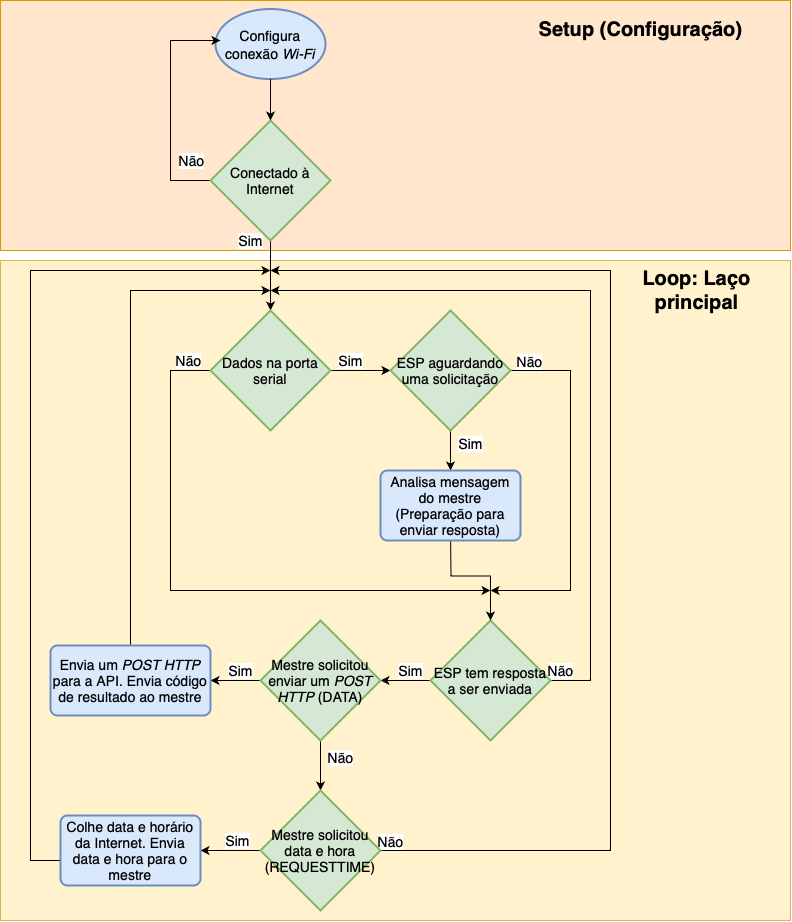
\includegraphics[width=0.5\linewidth]{aftertext//Firmware ESP8266/Figuras/ESP8266 Main flowchart (PT).png}
    \fonte{Desenvolvido pelo autor (2023)}
    \label{fig:fw-esp-main-flow}
\end{figure}

\section{Configuração e conexão \textit{Wi-Fi}}

Conforme mostra o fluxograma da \ref{fig:fw-esp-main-flow}, as primeiras ações que o programa executa são aquelas relacionadas ao estabelecimento da conexão à Internet via rede \textit{Wi-Fi} e a comunicação serial com o microcontrolador "mestre". Isso é realizado na função \texttt{setup()} conforme mostrado no código da Lista \ref{code:esp-setup}.

\begin{lstlisting}[language=C++, caption=Definição dos identificadores dos sensores de um dispositivo]
    void setup() 
    {
        Serial.begin(9600UL);
        Serial.print(F("+STARTESP;"));
        setup_wifi_connection<NUM_WIFIS>(wifiCreds);
        espHTTP.set_available(true);
        espSerial.set_status(WT_REQUEST);
        Serial.print(F("+ESPREADY;"));
    }
\end{lstlisting}
\label{code:esp-setup}

Primeiramente o programa inicializa a porta serial do ESP8266 a uma taxa de transmissão de 9600 bauds e imprime a mensagem \texttt{‘+STARTESP’}, indicando ao mestre que o programa foi inicializado. A função \texttt{setup\_wifi\_connection()} estabelece a conexão em uma rede \textit{Wi-Fi} previamente armazenada na variável \texttt{wifiCreds}. Por fim, uma vez estabelecida a conexão, o objeto \texttt{espSerial} que armazena o estado da comunicação serial é setado para \texttt{WT\_REQUEST} e a mensagem \texttt{'+ESPREADY'} é impressa, indicando que o ESP8266 está aguardando por uma solicitação do microcontrolador "mestre". A partir desse ponto o objeto \texttt{espHTTP} executa as requisições à \acrshort*{api} Renovar através do protocolo \textit{HTTP}. A continuação são descritos os objetos, constantes e funções usados nesta parte do código.

\subsection{\texttt{NUM\_WIFIS}}

Esta constante define a quantidade de redes \textit{Wi-Fi} com as quais o ESP8266 tentará estabelecer uma conexão. Esta constante deve ser declarada antes do objeto \texttt{wifiCreds} e antes de invocar a função \texttt{setup\_wifi\_connection()}.

\subsection{\texttt{WiFiCredentials wifiCreds[]}}

Esta variável é uma lista de objetos do tipo \texttt{WiFiCredentials}. Esta matriz armazena o \acrshort*{ssid} da rede, a senha e o nome de usuário (este último apenas em redes \textit{WPA3 ENTERPRISE}). A lista \texttt{wifiCreds} deve ser declarada antes da função \texttt{setup()}, conforme se mostra no códio da Lista \ref{code:esp-wifi-creds}. O tamanho da lista vai depender do valor da constante \texttt{NUM\_WIFIS}.

\begin{lstlisting}[language=C++, caption=Definição dos identificadores dos sensores de um dispositivo]
    /*Credenciais de uma rede empresarial WPA3*/
    const WiFiCredentials CRED_1("ssid1", "senha1", ENTERPRISE, "nomedeusuario1");

    /*Credenciais das redes pessoais WPA3*/
    const WiFiCredentials CRED_2("ssid2", "senha2", PERSONAL);
    const WiFiCredentials CRED_3("ssid3", "senha3", PERSONAL);

    /*Declara o array wifiCreds*/
    const WiFiCredentials wifiCreds[NUM_WIFIS] = { CRED_1, CRED_2, CRED_3 };
\end{lstlisting}
\label{code:esp-wifi-creds}

\subsection{\texttt{setup\_wifi\_connection<NUM\_WIFIS>(wifiCreds)}}

Esta função estabelece uma conexão a uma rede \textit{Wi-Fi}. É definido como um \textit{template} que recebe a quantidade de redes \textit{Wi-Fi} armazenadas em \texttt{wifiCreds}.

\subsection{\texttt{espHTTP}}

Esta variável é um objeto da classe \texttt{HTTPHandler}, definida no arquivo \texttt{esp-iot.h}, cujo objetivo é encapsular as funcionalidades relacionadas às operações \textit{HTTP}.

\subsection{\texttt{espSerial}}

Esta variável é um objeto da classe \texttt{ESPSerialHandler}, definida no arquivo \texttt{esp-serial-iot.h}. O objetivo deste objeto é encapsular as funcionalidades relacionadas à comunicação serial entre o ESP8266 e o microcontrolador mestre. Dependendo do estado deste objeto, o ESP8266 pode ler uma mensagem serial do mestre, ou executar uma determinada operação e enviar seu resultado de volta ao mestre. Para a versão atual do firmware, foram implementados dois estados:

\texttt{WT\_REQUEST}: Indica que o ESP8266 não recebeu nenhuma solicitação do mestre e está aguardando até receber uma nova.
\texttt{WT\_RESPONSE}: Indica que o ESP8266 recebeu alguma nova solicitação do mestre e está realizando as operações para enviar uma resposta.

\subsection{\texttt{Serial}}

Este é um objeto do framework Arduino para controlar a comunicação serial.

\section{O laço principal}

O laço principal do programa é executado dentro da função \texttt{loop()}, conforme mostrado no código abaixo. Esta função é responsável por monitorar a porta serial do ESP8266 e atender às solicitações do "mestre", conforme já ilustrado na Figura \ref{fig:fw-esp-main-flow}.

\begin{lstlisting}[language=C++, caption=Laço principal do programa]
void loop() 
{
    static CommandTypes _cmdType = ERROR;

    if(Serial.available())
    { 
        String serial_Str = Serial.readStringUntil(';');
        if(espSerial.get_status() == WT_REQUEST)  _cmdType = espSerial.parse(serial_Str);
        Serial.flush();
    }
    if(espSerial.get_status() == WT_RESPONSE)
    {
        espSerial.set_status(WT_REQUEST);
        switch (_cmdType)
        {
            case DATA:
            {
                static uint8_t _numberOfPostTries = 0;
                #define MAX_NUM_TRIES 3
                int code = espHTTP.post(HOST, PORT, URL, espSerial.get_data());
                
                if(code <= 0 && WiFi.status() != WL_CONNECTED)
                {
                    setup_wifi_connection<NUM_WIFIS>(wifiCreds);
                    if(++_numberOfPostTries >= MAX_NUM_TRIES-1) ESP.restart();
                }
                else  espSerial.send_http_code(code, Serial);
                break;
            }

            case REQUESTTIME:
            {
                static uint8_t _numberOfTries = 0;
                #define MAX_NUM_TRIES 3
                time_t t = get_time(TIMEZONE_SEC,DAYLIGTHOFFSET_SEC);
                if(!t && WiFi.status() != WL_CONNECTED)
                {
                    setup_wifi_connection<NUM_WIFIS>(wifiCreds);
                    if(++_numberOfTries >= MAX_NUM_TRIES-1) ESP.restart();
                }
                else  espSerial.send_time(t, Serial);
                break;
            }
            
            default:
            {
                break;
            }
        }
    }
}
\end{lstlisting}
\label{code:esp-loop}

\subsection*{Verificação das solicitações do "mestre"}

Sempre que houver dados na porta serial e o estado da comunicação serial (armazenado no objeto \texttt{espSerial}) for “aguardando solicitação” (\texttt{WT\_REQUEST}), o mesmo objeto \texttt{espSerial} analisará a cadeia de caracteres recebida do "mestre" para determinar o tipo de solicitação que recebeu. Isso é feito dentro do primeiro \texttt{if} da função \texttt{loop()}, conforme mostrado no código da Lista \ref{code:esp-serial-check}.

\begin{lstlisting}[language=C++, caption=Código para verificar as solicitações do mestre]
if(Serial.available())
{ 
    String serial_Str = Serial.readStringUntil(';');
    if(espSerial.get_status() == WT_REQUEST)  _cmdType = espSerial.parse(serial_Str);
    Serial.flush();
}
\end{lstlisting}
\label{code:esp-serial-check}

Uma vez analisada a mensagem do "mestre", \texttt{espSerial} definirá seu estado para “aguardando resposta” (\texttt{WT\_RESPONSE}), indicando que uma operação está em execução e uma resposta deve ser enviada de volta para o mestre (isso é feito internamente no a função parse). Se o status de \texttt{espSerial} for \texttt{WT\_RESPONSE}, o programa realizará uma operação \texttt{switch} para determinar qual operação o microcontrolador deve executar a seguir (fluxograma da Figura \ref{fig:fw-esp-main-flow}). A seleção da operação dependerá do tipo de solicitação enviado pelo mestre. O tipo de solicitação é armazenado na variável \texttt{\_cmdType} como resultado da operação \texttt{parse()} executada por \texttt{espSerial}. A Figura \ref{fig:fw-esp-comm-att} mostra esse processo.

\begin{figure}[h]
    \centering
    \caption{Processo de atendimento a uma solicitação do mestre}
    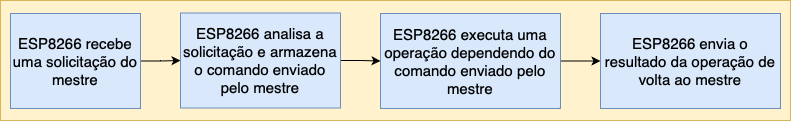
\includegraphics[width=0.9\linewidth]{aftertext//Firmware ESP8266/Figuras/ESP8266 sequence of comm operations (PT).png}
    \fonte{Desenvolvido pelo autor (2023)}
    \label{fig:fw-esp-comm-att}
\end{figure}

Na versão atual do firmware, o ESP8266 aceita dois tipos de solicitações ou comandos do mestre: (1) uma solicitação para enviar uma requisição à \acrshort*{api} Renovar via um \textit{POST HTTP} ou (2) uma solicitação de data e horário. A estrutura de uma mensagem de solicitação é mostrada no \acrshort{json} da Lista \ref{code:esp-wifi-json}. Depois que o objeto \texttt{espSerial} processa a mensagem do mestre, ele armazena o tipo de solicitação na variável \texttt{\_cmdType}. Esta variável é uma enumeração do tipo \texttt{CommandTypes} e, para a versão atual, pode conter os valores \texttt{ERROR}, \texttt{DATA} e \texttt{REQUESTTIME}, veja a Tabela \ref{tab:fw-esp-commands}.

\begin{lstlisting}[language=C++, caption=O formato da string JSON trocada entre o ESP8266 e o mestre]
{
    'type': // The type of the request. Could be 1 (DATA) or 2 (REQUESTTIME)
    'body': // The body of the request. Only used when the master is sending data (DATA)
}
\end{lstlisting}
\label{code:esp-wifi-json}

\begin{table}[h]
    \centering
    \caption{Tipos de solicitações representadas no tipo \texttt{CommandTypes}}
    \label{tab:fw-esp-commands}
    \begin{tabularx}{0.98\textwidth}[h]{
         >{\raggedright\hsize=.32\hsize\arraybackslash}X
         >{\raggedright\hsize=.12\hsize\arraybackslash}X 
         >{\raggedright\arraybackslash}X
         >{\raggedleft\hsize=.55\hsize\arraybackslash}X }
         \hline
         \texttt{CommandTypes} & \textbf{Valor}  & \textbf{Descrição} & \textbf{Resposta do mestre} \\
         \hline
         \texttt{ERROR} & 0 & Este comando indica que ocorreu um erro na comunicação do mestre com o ESP8266. Normalmente usado do ESP8266 para o mestre & É a resposta em caso de erro de comunicação \\
        \hline
        \texttt{DATA} & 1 & Este comando indica que o mestre enviou os dados para uma postagem HTTP e está aguardando o código HTTP retornado do servidor Web como resposta à postagem & O código HTTP retornado pelo servidor Web após a postagem \\
        \hline
        \texttt{REQUESTTIME} & 2 & Este comando indica que o mestre está solicitando a hora de um servidor NTP & O carimbo de data/hora obtido pelo servidor NTP \\
        \hline
    \end{tabularx}
    \fonte{Desenvolvido pelo autor (2023)}
\end{table}

\subsection{O comando \texttt{DATA}: enviando um \texttt{POST HTTP} para a API Renovar}

O código executado quando o "mestre" solicita o envio de um \textit{POST HTTP} é mostrado na Lista \ref*{code:esp-wifi-data-sequence}. O objeto \texttt{espHTTP} faz uma requisição tipo \textit{POST} para a \acrshort{api} hospedada em um servidor web identificado por um \textit{HOST} (hospedeiro), uma Porta e uma \acrshort{url} específica. Os dados enviados no \textit{POST} são os mesmos enviados anteriormente pelo mestre. Estes dados são acessados pelo método \texttt{get\_data()} de \texttt{espSerial}. O código retornado dessa operação é enviado como resposta ao "mestre" para manter controle das suas operações. Caso o código for de falha e o ESP8266 não estiver conectado à rede \textit{Wi-Fi}, o programa tentará se reconectar à rede e repassar os dados no máximo por três tentativas. Se, por outro lado, o código for de falha mas o ESP8266 estiver conectado a uma rede \textit{Wi-Fi}, o programa tentará enviar a mesma requisição indefinidamente até que o mestre envie uma nova solicitação. A Figura \ref*{fig:fw-esp-data-sequence} apresenta um fluxograma que representa esse processo. 

\begin{figure}[h]
    \centering
    \caption{Fluxograma do processo após uma solicitação de DATA do mestre.}
    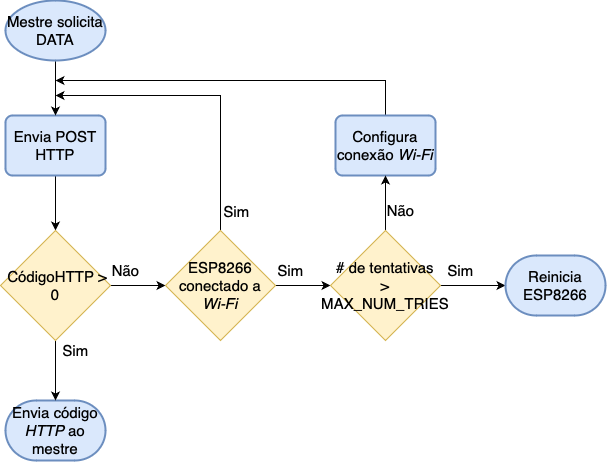
\includegraphics[width=0.75\linewidth]{aftertext//Firmware ESP8266/Figuras/ESP8266 DATA sequence (PT).png}
    \fonte{Desenvolvido pelo autor (2023)}
    \label{fig:fw-esp-data-sequence}
\end{figure}

\begin{lstlisting}[language=C++, caption=Sequencia de operações no comando DATA]
case DATA:
{
  static uint8_t _numberOfPostTries = 0;
  #define MAX_NUM_TRIES 3
  int code = espHTTP.post(HOST, PORT, URL, espSerial.get_data());
        
  if(code <= 0 && WiFi.status() != WL_CONNECTED)
  {
    setup_wifi_connection<NUM_WIFIS>(wifiCreds);
    if(++_numberOfPostTries >= MAX_NUM_TRIES-1) ESP.restart();
  }
  else  espSerial.send_http_code(code, Serial);
  break;
}
\end{lstlisting}
\label{code:esp-wifi-data-sequence}

Os valores de \texttt{HOST}, \texttt{PORT} e \texttt{URL} são definidos no arquivo \texttt{iot-generic.h} conforme se mostra abaixo; eles representam o \textit{endpoint} para enviar requisições à \acrshort*{api} Renovar.

\begin{lstlisting}[language=C++]
#define HOST  F("renovar.lcqar.ufsc.br")
#define PORT  8080UL
#define URL   F("/sample/")
\end{lstlisting}

\subsection*{O comando \texttt{REQUESTTIME}: obtendo a hora de um servidor \acrshort*{ntp}}

O código executado quando o ESP8266 recebe uma solicitação de horário é mostrado na Lista \ref*{code:esp-wifi-time-sequence}. A função \texttt{get\_time()} é definida no arquivo \texttt{esp-iot.h} para obter a data e hora atuais desde um servidor 
\acrshort{ntp}. O valor retornado dessa operação é enviado como resposta ao "mestre". Caso o valor for zero e o ESP8266 não esteja conectado à rede \texttt{Wi-Fi}, o programa tentará se reconectar à rede e obter o horário da Internet por no máximo três tentativas. Por outro lado, se o valor for zero, mas o ESP8266 estiver conectado a uma rede Wi-Fi, o programa tentará obter o horário da Internet indefinidamente até receber uma nova solicitação. A Figura \ref*{fig:fw-esp-time-sequence} apresenta um fluxograma que representa esse processo.

\begin{figure}[h]
    \centering
    \caption{Fluxograma do processo após uma solicitação TIME do mestre}
    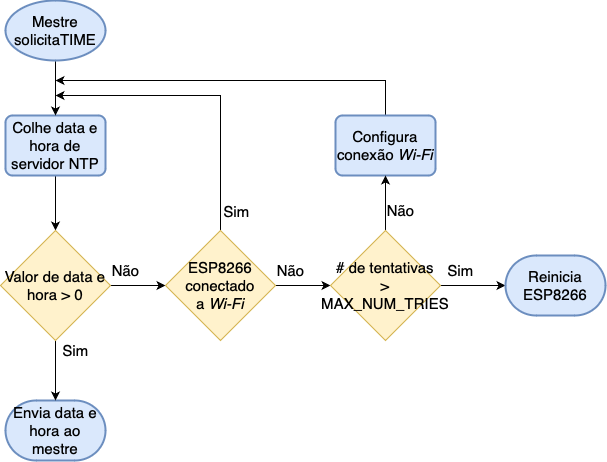
\includegraphics[width=0.75\linewidth]{aftertext//Firmware ESP8266/Figuras/ESP8266 TIME sequence(PT).png}
    \fonte{Desenvolvido pelo autor (2023)}
    \label{fig:fw-esp-time-sequence}
\end{figure}

\begin{lstlisting}[language=C++, caption=Sequencia de operações no comando REQUESTTIME]
case REQUESTTIME:
{
  static uint8_t _numberOfTries = 0;
  #define MAX_NUM_TRIES 3
  time_t t = get_time(TIMEZONE_SEC,DAYLIGTHOFFSET_SEC);
  if(!t && WiFi.status() != WL_CONNECTED)
  {
    setup_wifi_connection<NUM_WIFIS>(wifiCreds);
    if(++_numberOfTries >= MAX_NUM_TRIES-1) ESP.restart();
  }
  else  espSerial.send_time(t, Serial);
  break;
}
\end{lstlisting}
\label{code:esp-wifi-time-sequence}

A função \texttt{get\_time()} recebe os parâmetros \texttt{TIMEZONE\_SEC} e \texttt{DAYLIGTHOFFSET\_SEC}, definidos anteriormente no arquivo \texttt{main.cpp}. O exemplo abaixo mostra como definir esses dois parâmetros para a aplicação no Brasil. \texttt{TIMEZONE\_SEC} é o fuso horário onde o monitor será instalado, convertido a segundos. \texttt{DAYLIGTHOFFSET\_SEC} define o deslocamento, em segundos, para o horário de verão, nesse caso foi definido como zero.

\begin{lstlisting}[language=C++]
#define TIMEZONE_SEC        -3*3600
#define DAYLIGTHOFFSET_SEC  0*3600
\end{lstlisting}
\end{apendicesenv}
% ---


% ----------------------------------------------------------
% Anexos
% ----------------------------------------------------------

% ---
% Inicia os anexos
% ---
\begin{anexosenv}
%	\partanexos*
	% ----------------------------------------------------------
\chapter{Descrição}
% ----------------------------------------------------------

São documentos não elaborados pelo autor que servem como fundamentação (mapas, leis, estatutos). Deve ser precedido da palavra ANEXO, identificada por letras maiúsculas consecutivas, travessão e pelo respectivo título. Utilizam-se letras maiúsculas dobradas quando esgotadas as letras do alfabeto. 

\end{anexosenv}

%---------------------------------------------------------------------
% INDICE REMISSIVO
%---------------------------------------------------------------------
%\phantompart
%\printindex
%---------------------------------------------------------------------

\end{document}
